%
%  --- USU thesis and dissertation template ---
%
% Time-stamp: "[thesis.tex] last modified by Scott Budge (scott) on 2012-11-01 (Thursday, 1 November 2012) at 10:15:42 on goga.ece.usu.edu"
%
%  Modified to use the new usuthesis.cls by Allan McInnes
%
%  Specify department ('ee' or 'ce' or 'mae') and document type ('msthesis',
%  'msreport', or 'dissertation') in the documentclass options. 
%
%  Including the 'proposal' option will generate a proposal for a thesis
%  or dissertation, rather than a final document (this mostly just 
%  alters the cover page).
%
%  See the opening comments of usuthesis.cls for more information on 
%  available options
%
%  To create finished document run:
%    latex thesis.tex
%    bibtex thesis (or sample-chapter1, etc., if using multiple-paper format)
%    latex thesis.tex
%    latex thesis.tex
%
%  Info: $Id$   USU
%  Revision: $Rev$
% $LastChangedDate$
% $LastChangedBy$
%

\documentclass[ee,msthesis]{usuthesis}

%{{{ Packages
\usepackage{amsmath}
\usepackage{amssymb}           % add ams symbols stuff
\usepackage{graphicx}          % add graphics
\usepackage{epstopdf}
\graphicspath{{./figures/}} 
\usepackage{subfig}
\usepackage{url}
\usepackage{flafter}           % Cause floats to appear after
                               % environment.
%\usepackage{siunitx}           % Provides standard formatting of SI units.
%\usepackage{hyperref}
%\usepackage{xr}
%\usepackage{boxedminipage}
\usepackage{listings}
\usepackage[shortlabels]{enumitem}
\usepackage{tikz}
\usepackage{tkz-euclide}
\usetkzobj{all}
% Include TikZ and PGF packages for high-quality graphics, schematics
% and plots. This is optional; at the current time, when run with
% latex to create a .dvi file, the xdvi viewer will produce incorrect
% formatting for the TikZ figures.  If the .dvi file is converted to
% pdf using "dvipdf" the resulting pdf file is correct.  If this
% example is used with  pdflatex, the resulting TikZ figures in the
% output look fine.
\usepackage{tikz}       		% The base tikz+pgf package
\usetikzlibrary{arrows,shapes}	% Optional tikz extentions
\usepackage[american]{circuitikz}	% TikZ-based package for schematic drawings
\usepackage{pgfplots}			% Tikz-based package for making plots 
\pgfplotsset{compat=1.6}        % This *might* be necessary for your
                                % version of pgfplots.

% The following is added if you are using the multiple-paper format to
% add references after each chapter:
%\usepackage[sectionbib]{chapterbib}

%}}}

% Author and Title Information
\author{Roque Lora}
\title{Unmanned Aerial Vehicle Tracking System with Out-Of-Sequence Measurement in a Discrete Time-Delayed Extended Kalman Filter}

% The Committee
\majorprof{Dr. Rajnikant Sharma}
\firstreader{Dr. Rees Fullmer}
\secondreader{Dr. Todd K. Moon}

% Graduate Dean
\graddean{Dr. Mark R. McLellan}
\deantitle{Vice President for Research and \\
Dean of the School of Graduate Studies}

% Degree Information
\degree{Master of Science}
\month{October}
\gradyear{2014}

\begin{document}
    %{{{ Frontmatter
    \preliminaries   % set frontmatter style
    
    \maketitle
    \makecopyright        % optional
    
    %
%  Time-stamp: "[abstract.tex] last modified by Scott Budge (scott) on 2011-08-08 (Monday, 8 August 2011) at 15:44:55 on goga"
%
%  Info: $Id$   USU
%  Revision: $Rev$
% $LastChangedDate$
% $LastChangedBy$
%

\begin{abstract}
% A space is needed before the text starts so that the first paragraph
% is indented properly.

This extends the delayed Kalman filter to a delayed extended Kalman filter that takes into account the delays of the measurement. The filter uses GPS and camera measurements for the estimation of the states of an unmanned aerial system (UAS). The GPS output is delayed by a random number, which produces the out-of-sequence measurement problem. The filter is based on calculating the states with the measurements at the moment, so that when the delayed measurements are available, the optimal filter for the time of the measurement is calculated and propagated to the present time. The estimates provided by the filter are used to point an antenna and a camera towards the UAS.

\end{abstract}


% Local Variables:
% TeX-master: "newhead"
% End:

    %
%  Time-stamp: "[publicabstract.tex] last modified by Scott Budge (scott) on 2011-08-09 (Tuesday, 9 August 2011) at 09:17:43 on goga"
%
%  Info: $Id$   USU
%  Revision: $Rev$
% $LastChangedDate$
% $LastChangedBy$
%

\begin{publicabstract}
% A space is needed before the text starts so that the first paragraph
% is indented properly.

The goal of this thesis is to extend the delayed Kalman filter so it can be used with non-linear systems and that it can handle randomized delays on the measurements. In the particular case of this study, the filter is used to estimates the states of an unmanned aerial system, The outputs of the filter are used to point an antenna and a camera towards a UAS. Different scenarios are simulated for the purpose of comparing the efficiency of this technique in various situations. 

\end{publicabstract}


% Local Variables:
% TeX-master: "newhead"
% End:

    %
% This is an example of an dedication page.  This is optional,
% and can contain anything you want to say.
%
%  Time-stamp: "[dedication.tex] last modified by Scott Budge (scott) on 2011-08-08 (Monday, 8 August 2011) at 15:46:26 on goga"
%
%  Info: $Id$   USU
%  Revision: $Rev$
% $LastChangedDate$
% $LastChangedBy$
%

\begin{dedication}
\begin{center} 
To God, my wife, Dr. Sharma, my family, AggieAir, and all my friends.
\end{center}
% 
% If you intend to have a dedication longer than one line, do not put
% it in a centering environment.  It will look better.
\end{dedication}
  % optional 
    %
% This is an example of an acknowledgements page.  This is optional,
% and can contain anything you want to say.
%
%
%  Time-stamp: "[acknowl.tex] last modified by Scott Budge (scott) on 2011-08-08 (Monday, 8 August 2011) at 15:45:15 on goga"
%
%  Info: $Id$   USU
%  Revision: $Rev$
% $LastChangedDate$
% $LastChangedBy$
%

\begin{acknowledgments} 

I want to acknowledge God, as the one that gave me the opportunity and strength to reach this milestone in my life. My wife, who was the biggest pillar in my life during the whole master. She always supported me giving me strength during the successes and failures and was the one that comforted me when I felt frustrated. She is the main source of my inspiration. Dr. Sharma, who made this whole research possible. Dr. Sharma took me as his student since he arrived at USU, even when I did not have a clear subject for my research. He dedicated countless hours of his time to polish and guide me through this whole research. I am very grateful for his support, patience and the knowledge that he shared with me. To my family, who gave me support and believed in me since day one. To AggieAir, who taught me so much and helped me developed as a professional. And to all the friends that made this whole experience unforgettable.

\bigskip

Thank you,

\begin{flushright} 
	Roque Lora 
\end{flushright}

\end{acknowledgments}

     % optional
    
    \tableofcontents 
    %\listoftables 
    \listoffigures
    
%    %
%  Time-stamp: "[notation.tex] last modified by Scott Budge (scott) on 2011-08-08 (Monday, 8 August 2011) at 15:48:03 on goga"
%
%
% This is an example of a notations page.  
% The publication guide does not specify a format.
% The example here is in tabular format.
%
% Please note that the symbols in this example are defined
% in a separate include file.
%  Info: $Id$   USU
%  Revision: $Rev$
% $LastChangedDate$
% $LastChangedBy$
%

\begin{notation}

\setlength{\tabcolsep}{3mm}
{\begin {tabular}{ll}
\multicolumn{2}{l}{\textbf{Events}}\\
$\Sigma$ & set of all events (universal alphabet)\\
$\tick$   & successful termination signal\\
$\tau$ & invisible (internal) event\\
$a.b.c$    & compound event\\
$c ? x$   &input on channel $c$\\
$c ! x$   &output on channel $c$\\
$\lchan c \rchan$   &set of all events associated with channel $c$\\
\multicolumn{2}{l}{\textbf{Traces}}\\
$\nil$ &empty sequence\\
$\lseq a_1, \ldots , a_n \rseq$ & sequence $a_1, \ldots , a_n$, in that order\\
$s_1 \cat s_2$ &$s_1$ concatenated with $s_2$, e.g. $\lseq a \rseq \cat \lseq b \rseq = \lseq a, b \rseq$\\
$s_1 \leq s_2$ &$s_1$ is a prefix of $s_2$, e.g.  $\lseq a \rseq \leq \lseq a, b \rseq$ \\
$s \hide X$ &hiding - all members of $X$ removed from $s$\\
$s \restrict X$ &restriction - hide all but members of $X$\\
$s \crestrict c$ &sequence of values in $s$ communicated over channel $c$\\
$s \seqcount a$ &number of $a$ events in $s$\\
\multicolumn{2}{l}{\textbf{Processes}}\\
$a \then P$ &prefixing\\
$P \interleave Q$ &interleaved parallel\\
$P \parallel[A][B] Q$ &alphabetized parallel\\
$P \parallel[X] Q$ &interface parallel\\
$P \extchoice Q$ &external choice\\
$P \intchoice Q$ &nondeterministic choice\\
$P \comp Q$ &sequential composition\\
$P \hide X$ &hiding\\
\end {tabular}}

% The table as defined above will fill one page. If you need more room to list
% notation you will need to create a second table, and place it below this 
% comment. This new table will appear one a new page.

\end{notation}

  % optional
    %
% This is an example of an acronyms page.  
% Acronyms are laid out in tabular format.
%
%  Time-stamp: "[acronyms.tex] last modified by Scott Budge (scott) on 2011-08-08 (Monday, 8 August 2011) at 15:45:41 on goga"
%
%  Info: $Id$   USU
%  Revision: $Rev$
% $LastChangedDate$
% $LastChangedBy$
%

\begin{acronyms}

\renewcommand{\arraystretch}{1.5}
\setlength{\tabcolsep}{3mm}
{\begin {tabular}{ll}
DEKF  &Delayed Extended Kalman Filter\\
DOP   &Dilution Of Precision \\
EO	  &Electro-Optical \\
EKF   &Extended Kalman Filter\\
FAA   &Federal Aviation Administration \\
GCS   &Ground Control Station \\
GPS   &Global Positioning System \\
IMU   &Inertial Measurement Unit \\
IR    &Infrared \\
KF   &Kalman Filter\\
LOS  &Line-of-Sight\\
MSE   &Mean Squared Error \\
OOSM  &Out Of Sequence Measurement \\
UAS  &Unmanned Aerial System\\
UAV  &Unmanned Aerial Vehicle\\


%CSOIS &Center for Self-Organizing and Intelligent Systems\\

\end {tabular}}

\end{acronyms}
  % optional     
    \body  % set main body style
    % Chapters
    \chapter{Introduction}
\label{ch:introduction}

\section{Background}
Recently the use of unmanned aerial systems (UAS) has increased dramatically in both civilian and military applications. Because of this, the Federal Aviation Administration (FAA) has been modifying the requirements for the operation of UAS. The one that concerns us is the line-of-sight (LOS) requirement, which constrains the aircraft mission to be within the visual field of the operator. The existing method is to keep an eye on the aircraft with binoculars, which is prone to lose the plane frequently. The importance of UAS tracking systems relies on having a good link between the aircraft and the ground control station (GCS), which can be assured using a good antenna pointing system.

Another critical requirement in the reliability of a UAS mission is the communication with the ground station. For reliable communication it is necessary to point the antenna towards the UAS and maintain the LOS with the aircraft. Therefore, the communication link will be strong as long as we have LOS. This is apparent for applications that require real-time feedback, because if the tracking of the UAS is not accurate, the link could be interrupted and no feedback would be sent back. An example is a military mission where an aircraft supports an advancing troop in enemy territory.  The decisions made by the leader of the troop are greatly influenced by the feedback of the UAS. If the communication between the UAS and the GCS is lost, there would not be any feedback from the UAS and the safety of the soldiers could be compromised. Moreover, in a civilian application such as disaster relief for an earthquake, the aircraft could be equipped with a thermal imaging camera to detect heat sources. It would identify warm bodies under the rubble in real time so the help could get there as soon as possible. If the communication is lost between the UAS and the GCS, some information might be missed that could lead to the detection of a survivor.

\section{Contributions}
\begin{figure}[h!]
  \centering
  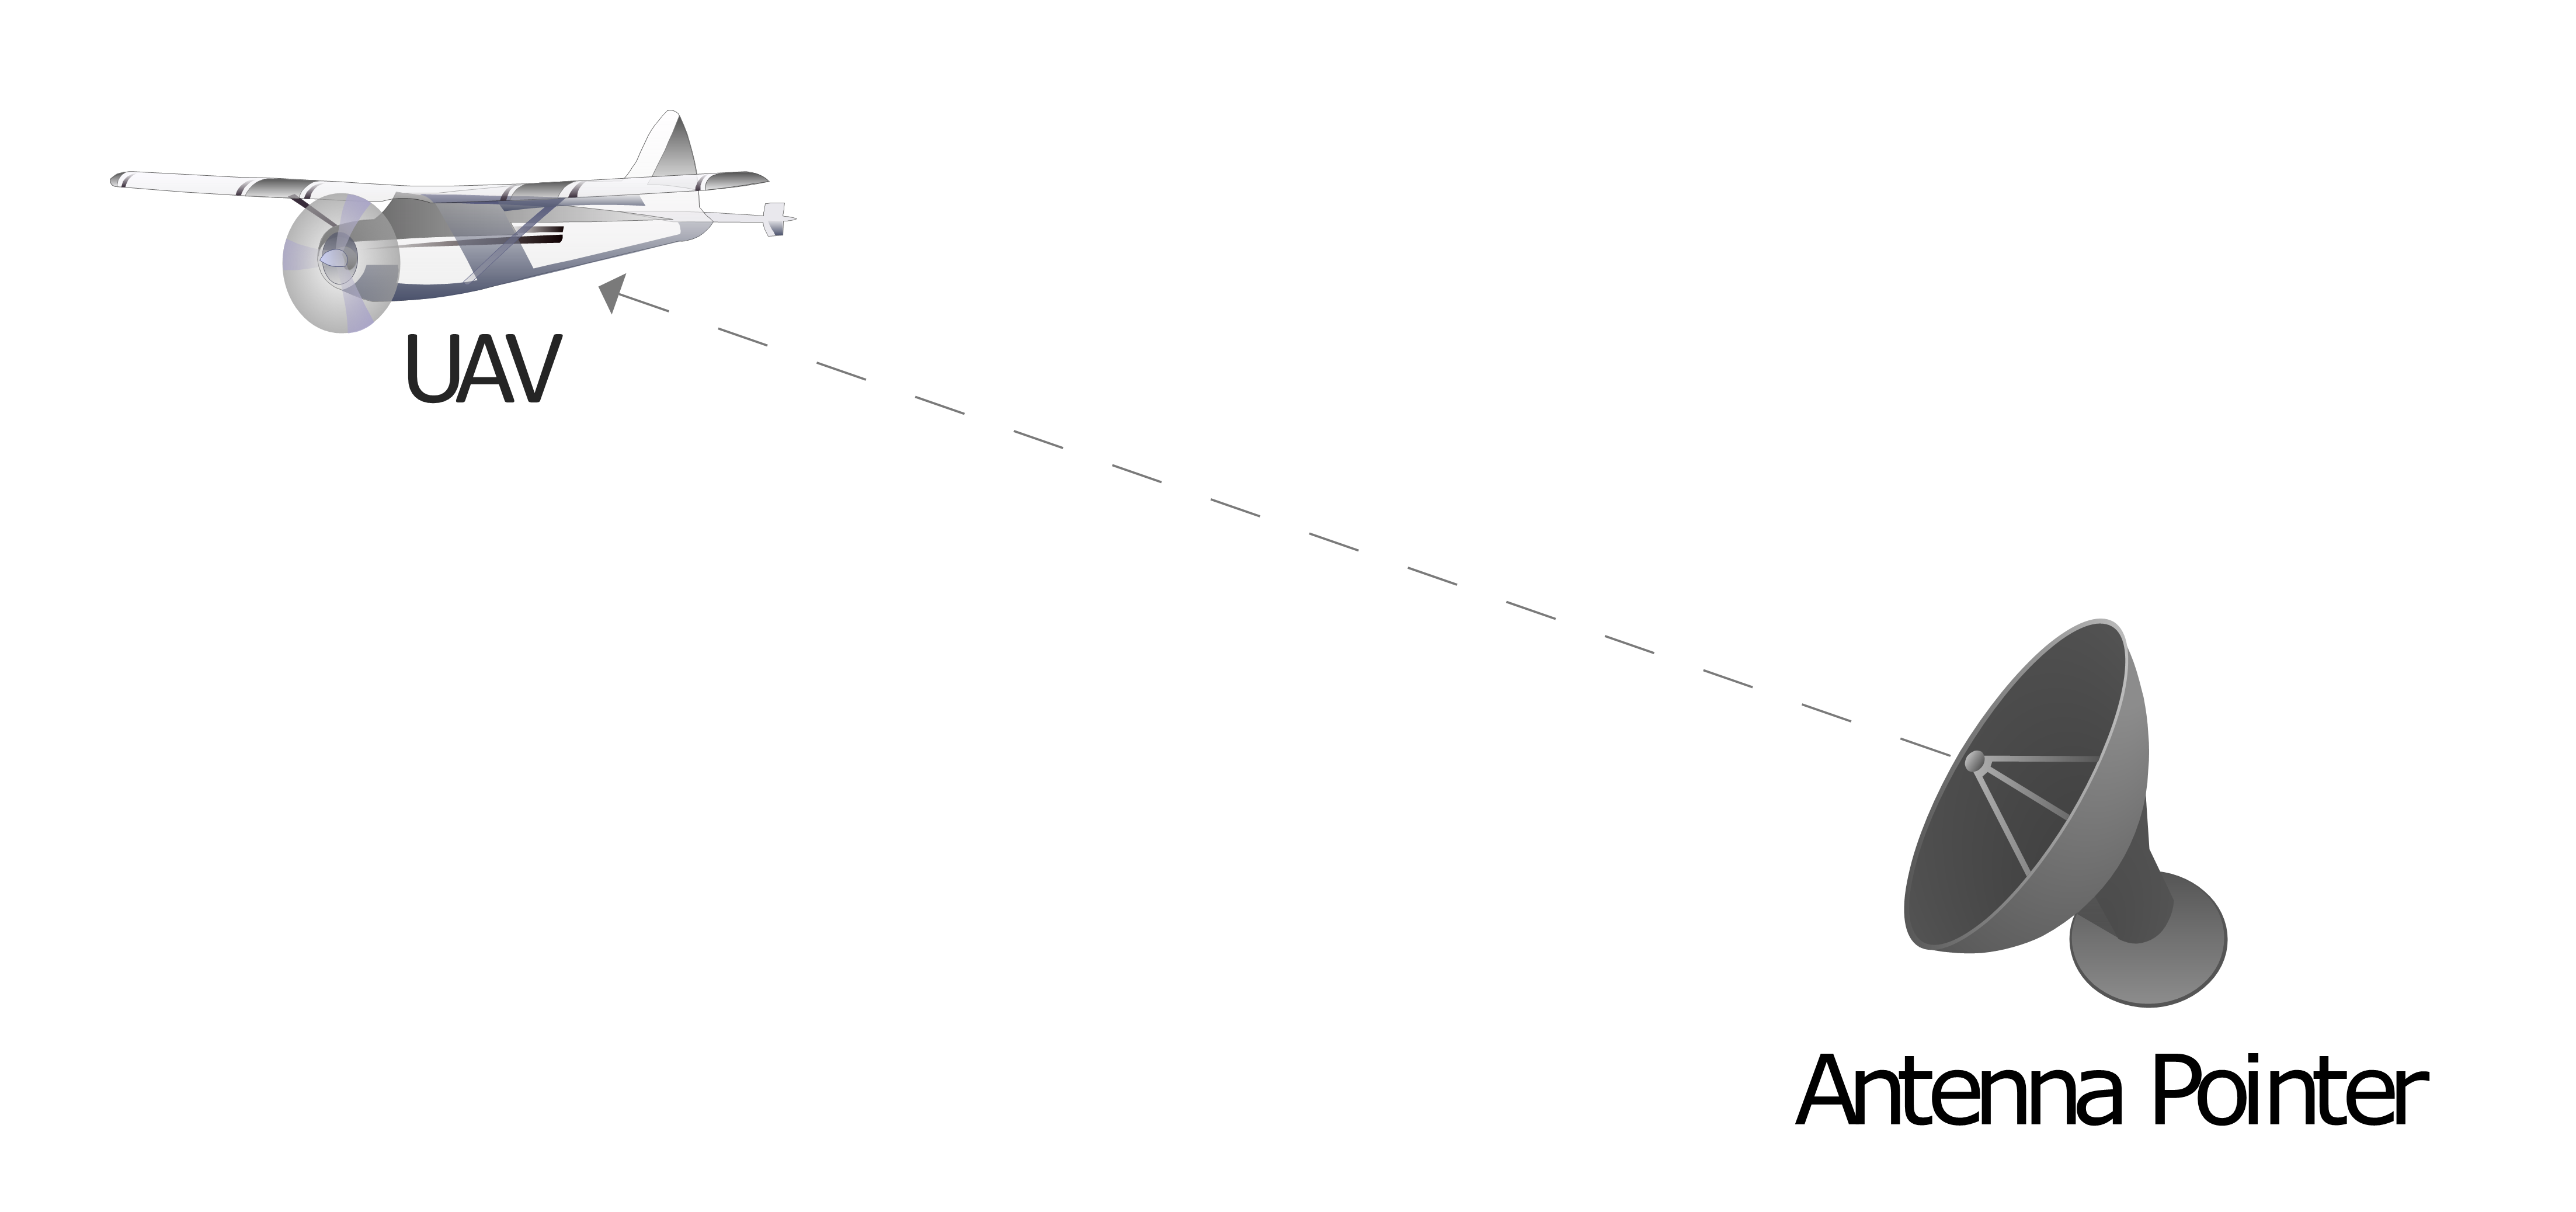
\includegraphics[scale=.075]{./Diagrams/AP_UAV}
  \caption{Antenna Pointer tracking an UAS}
\end{figure}
The main focus of this work is to design an autonomous system to point an antenna mounted with a camera towards a flying UAS to maintain communication and visual LOS to satisfy FAA requirements. In order to point a camera, the precise position of the aircraft is required. The existing approach is for the GCS to use the position obtained from a GPS receiver on board the UAS. There are several limitations of this approach. 
\begin{itemize}[nosep]
\item The GPS receives position updates at 1-4 Hz, not fast enough to point the antenna towards an UAS flying at 20 m/s.
\item The position updates at the antenna are delayed and have out-of-sequence measurements (OOSM) due to communication delays.
\end{itemize}
\begin{figure}[h!]
  \centering
  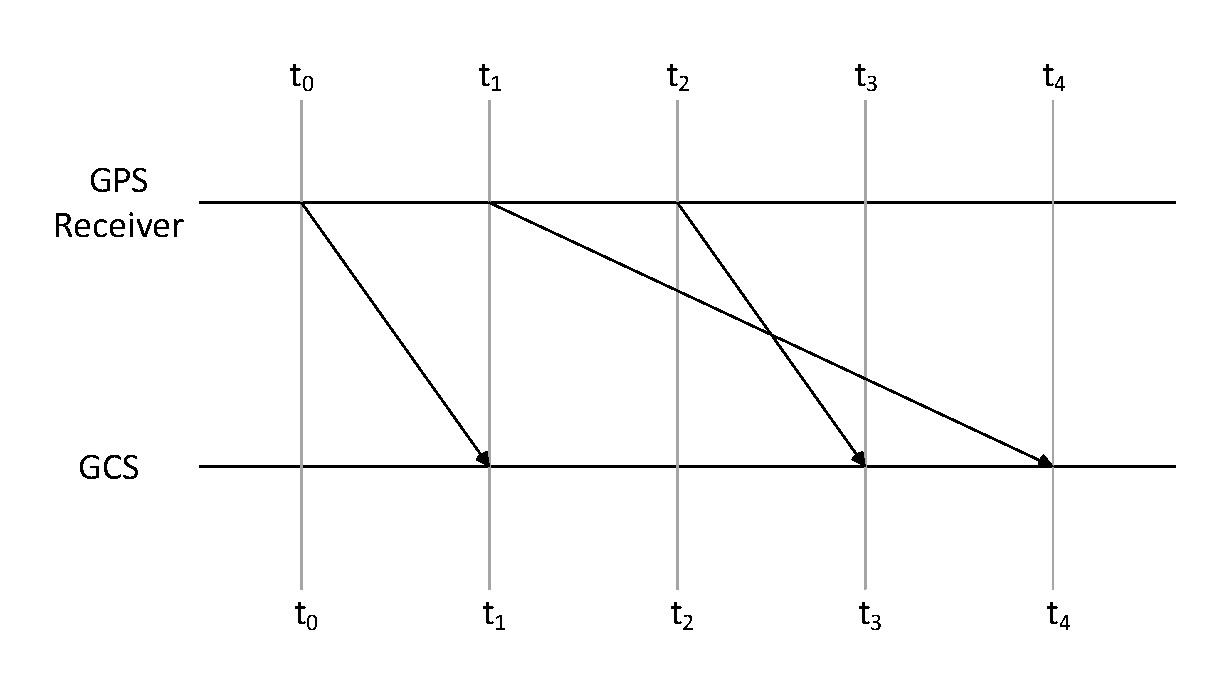
\includegraphics[scale=.37]{./Diagrams/OOSM}
  \caption[Out-Of-Sequence Measurement]{OOSM. 
  In this diagram the generation time of various measurements (GPS receiver line) and the time that they are available to the system (GCS line) are shown. Measurements $t_1$ and $t_2$ are out-of-sequence since $t_2$ is available first than $t_1$.\label{fig:OOSM}}
\end{figure}
A measurement is called out-of-sequence if it is available to a processing unit first than another measurement taken in an earlier time step. This situation is shown in figure \ref{fig:OOSM}.

The first problem is addressed by adding a camera which provides location measurements from images of the aircraft at 30 Hz, compensating the slow update rate of GPS. However, the camera's accuracy deteriorates with distance, since at higher distances the aircraft would only be a couple of pixels in the camera image, making the recognition of the UAS impossible. On the other hand, GPS measurements' errors are independent of the distance between the fixed wing and the antenna pointer, making the relative error smaller at higher distances. Hence, we can say that the camera and GPS are complementary sensors for pointing the antenna. The second problem of receiving out of sequence measurements is addressed by using an extended Kalman filter which uses out of sequence GPS measurements with camera measurements to estimate the position of the UAS. This estimation is then used to reliably point the antenna and camera towards the aircraft.

\pagebreak
\section{Literature Review}
For more than two decades, the problem of OOSM have been addressed in several different ways. The initial studies about the OOSM are presented in \cite{Hilton1993} in 1993, where a negative-time update technique is developed using the criterion of minimum mean-square error. The first optimal algorithm for the general multi-step lag problem appeared in \cite{Nettleton2001} in 2001. It consisted in buffering all the measurements received and running the filter behind real-time. Consequently, this algorithm is not able to run in real time. In \cite{Larsen1998}, a solution of this problem is presented, in which a new filter is developed where the measurements are extrapolated forward in time using past and present estimates to calculate an optimal gain for the Kalman filter. The work of \cite{Larsen1998} is expanded in \cite{Julier2005}, where a covariance union method is proposed to solve the multi-lag OOSM when the delay is not precisely known. In \cite{Mallick2001} a linear minimum variance estimation algorithm was extended to handle multiple lags and dynamics models. This exposed that as the number of lags increases, the state estimation accuracy decreases. The same problem is addressed in \cite{Bar-Shalom2002a}. The one-step lag OOSM solution is generalized to solve problems when multiple lags arise. This extension comes with a significantly lower storage requirement and a small (1\%) degradation of MSE performance. A two-step method was presented in \cite{Lanzkron2004} which requires one more step to update the state at the OOSM time. Two optimal algorithms were presented in \cite{Zhang2002} to approach the multi-step OOSM problem using fixed-point smoothing. It was shown that both of these algorithms are flexible and relatively simple but highly computationally demanding. In \cite{Bar-Shalom2002} the exact state update equation for the OOSM problem is presented and compared to two suboptimal algorithms. Each method is tied to the situations where they should be used comparing simplicity against optimality. A smoothing-based algorithm was proposed in \cite{Mallick2002} in the case of multi-sensor multi-target ground moving target tracking problem. It concluded that discarding OOSM can lead to severe degradation in the state estimation. Also these two methods have better accuracy than the previous buffering method approach. A unified sub-optimal Bayesian approach is proposed in \cite{Challa2002} for the multi-lag OOSM problem. This algorithm, developed on the basis of a fixed-lag smoothing framework and its solution reduces to an augmented state Kalman filter. An extension of the particle filter approach can be found in \cite{Orton2005} where it compares it results with the extended Kalman filter, showing that both have similar performance. The work of \cite{Plett2007} develops an out-of-order sigma-point Kalman filter for solving the multi-lag OOSM in a single measurement vector and using the batch-form update. This method is equivalently complex per iteration as the sigma-point Kalman filter but it requires more iterations. An extended Kalman filter was used to estimate the position of a UAS using a camera and then coupled with an inertial measurement unit (IMU). The results shown that coupling the camera with an IMU reduces the position estimation error by almost and order of magnitude, compared to using only the camera \cite{Kelly2008}. In \cite{Zhang2012} three different approaches were proposed to achieve optimality. The study yielded that the complete in-sequence information fixed point smoothing method was the optimal approach, but it lacks simplicity. 

The work of this thesis is developed by combining the delayed Kalman filter of \cite{Larsen1998} and the extended Kalman filter explained in \cite{Beard2010a}. Both techniques are combined in a filter with a nonlinear model of the system that can handle delays. Moreover, random delays and the OOSM problem will be handled by the modified filter. The estimation errors will be compared for different GPS measurement delays, fixed and randomized, as well as using GPS alone or coupled with a camera. Also, for comparison purposes, the estimation is done by an extended Kalman filter which will not take into account the delays or the OOSM problem. Therefore, the major contribution of this study is to clearly show the increase in accuracy that comes from using this delayed extended Kalman filter.
    \include{background}
    \chapter{Sensors and Kalman Filters}{\label{ch:Sensors}}
In this chapter we explain the required elements for the antenna pointer system. The first requirement to track a UAS is some information about its position. This data is provided by a GPS mounted in the aircraft and a camera mounted in the antenna pointer. These sensors are low cost and are very common in unmanned aircraft systems. The combination of these sensors is due to the characteristics of them. Since the GPS measurement errors are independent of the distance between the aircraft and the antenna pointer, it is relatively accurate at medium and long distances, but not at short range. By contrast, the camera can estimate correctly the position of an object within short range, but at medium and long distances it can not detect the target since it is just a few pixels in the image, therefore at long distances it is practically unusable. Furthermore, the GPS has an update frequency of 1 Hz to 4 Hz, while cameras can sample from 5 Hz to more than 20 Hz. In section \ref{sect:GPS} we explain how GPS works and provide an algorithm to estimate the states of a UAS. Then in section \ref{sect:camera} we present the camera model used for this simulation, and some coordinates frames that we use to geolocate a target based on camera images. Also a simple algorithm for pointing the antenna towards the UAS is shown.

The second requirement of our system is the ability to process the information received from both sensors to fuse the data and improve the estimation of the states of the UAS. For this purpose, a Kalman filter is used. In section \ref{sect:kalman_filter} we explain briefly the basic Kalman filter. Later on, the extended Kalman filter is presented. Different reasons can cause delays on the measurements. Therefore, an algorithm called delayed extended Kalman filter is explained, which takes in consideration the time lag on the measurements and compensates for it to produce a better estimation of the states.

\pagebreak
\section{Aircraft Dynamics}
12-state equations of motion
\begin{align*}
\dot{p_n}&=(\cos\theta\cos\psi)u+(\sin\phi\sin\theta\cos\psi-\cos\phi\sin\psi)v\\
&\quad+(\cos\phi\sin\theta\cos\psi+\sin\phi\sin\psi)w \\
\dot{p_e}&=(\cos\theta\sin\psi)u+(\sin\phi\sin\theta\sin\psi+\cos\phi\cos\psi)v\\
&\quad+(\cos\phi\sin\theta\sin\psi-\sin\phi\cos\psi)w \\
\dot{h}&=u\sin\theta-v\sin\phi\cos\theta-w\cos\phi\cos\theta\\
\dot{u}&=rv-qw-g\sin\theta\\
&\quad+\frac{\rho V_a^2S}{2m}[C_X(\alpha)+C_{X_q}(\alpha)\frac{cq}{2V_a}+C_{X_{\delta_e}}(\alpha)\delta_e]\\
&\quad+\frac{\rho S_{prop}C_{prop}}{2m}[(k_{motor\delta_t})^2-V_a^2]\\
\dot{v}&=pw-ru+g\cos\theta\sin\phi+\frac{\rho V_a^2S}{2m} \\
&\quad\times[C_{Y_0}+C_{Y_\beta}\beta+C_{Y_p}\frac{bp}{2V_a}+C_{Y_r}\frac{br}{2V_a}+C_{Y_{\delta_a}}\delta_a+C_{Y_{\delta_r}}\delta_r]\\
\dot{w}&=qu-pv+g\cos\theta\cos\phi\\
&\quad+\frac{\rho V_a^2S}{2m}[C_Z(\alpha)+C_{Z_q}(\alpha)\frac{cq}{2V_a}+C_{Z_{\delta_e}}(\alpha)\delta_e]\\
\dot{\phi}&=p+q\sin\phi\tan\theta+r\cos\phi\tan\theta \\
\dot{\theta}&=q\cos\phi-r\sin\phi \\
\dot{\psi}&=q\sin\phi\sec\theta+t\cos\phi\sec\theta\\
\dot{p}&=\Gamma_1pq-\Gamma_2qr+\frac{1}{2}\rho V_a^2Sb \\
&\times[C_{p_0}+C_{p_\beta}\beta+C_{p_p}\frac{bp}{2V_a}+C_{p_r}\frac{br}{2V_a}+C_{p_{\delta_a}}\delta_a+C_{p_{\delta_r}}\delta_r]\\
\dot{q}&=\Gamma_5pr-\Gamma_6(p^2-r^2)+\frac{\rho V_a^2Sc}{2\mathcal{J}_y}\\
&\quad\times[C_{m_0}+C_{m_\alpha}\alpha+C_{m_q}\frac{cq}{2V_a}+C_{m_{\delta_e}}\delta_e]\\
\dot{r}&=\Gamma_7pq-\Gamma_1qr+\frac{1}{2}\rho V_a^2Sb\\
&\quad\times[C_{r_0}+C_{r_\beta}\beta+C_{r_p}\frac{bp}{2V_a}+C_{r_r}\frac{br}{2V_a}+C_{r_{\delta_a}}\delta_a+C_{r_{\delta_r}}\delta_r]
\end{align*}

\pagebreak
\section{Global Positioning System}{\label{sect:GPS}}

The global positioning system (GPS) is a navigation system supported by satellites that provides location information for objects on or near the surface of the earth. The navigation satellite timing and ranging (NAVSTAR) GPS has been functioning since 1993 and was developed by the United States Department of Defense. The GPS is one of the most important technologies that allows the functioning of UAS, giving them spatial localization. A more detailed description of the global navigation satellite systems can be found in many texts such as \cite{Zogg2009}, \cite{Parkinson1996}, \cite{Parkinson1996a}, \cite{Kaplan2005}, and \cite{Grewal2007}. In this section we explain briefly how the sensing works in GPS systems and we present a GPS model appropriate for simulation.

The most important element in the GPS system is the 24 satellites that orbit continuously around the earth at an altitude of 20,180 km \cite{Zogg2009}. The constellation of the satellites orbits is configured so that any location on the surface of the earth can be observed by at least four satellites all the time. It is common knowledge that with one range measurement is possible to locate a point in a line. With two range measurements a point on a plane and with three range measurements, a point on a 3-D surface. This explains the need for three of the four satellites. But the last one comes from clock synchronization errors between the satellites and the receiver. Therefore, with four independent pseudo-range measurements, there exists a system of four nonlinear equations which yield to the solution of the four variables of interest: latitude, longitude, altitude and receiver clock time offset \cite{Zogg2009}. This section is based on the work of \cite{Beard2010}.

\subsection{GPS Measurement Error Model}{\label{sub:gps_meas_error}}
The two factors that affect the precision of a GPS position measurement are the accuracy of the satellite pseudo-range measurements and the configuration of the satellites from which these pseudo-measurements are taken. The first factor is impacted by errors in the time of flight for each satellite. Where the second one is considered in a term called dilution of precision (DOP).
\pagebreak
\subsubsection{Standard Pseudo-Range Error Sources}
\paragraph{Ephemeris Data} \hspace{0pt} \\
The satellite ephemeris gives the position of the satellite in the sky at a given time. The position of the GPS receiver is calculated using measurement ranges with respect to satellites. To determine this position, we are required to know the locations of the satellites in the first place. Ephemeris errors in the measurements exists because of the inaccuracies in the transmitted orbital satellite location. Common errors vary from 1 to 5 m.

\paragraph{Satellite Clock} \hspace{0pt} \\
The atomic clocks used in GPS satellites are made of cesium and rubidium. These clocks can drift about 10 ns a day. This translates to an error of 3.5 m. But their clocks are synchronized twice a day, therefore leading to an approximately 1.75 m error.

\paragraph{Ionosphere} \hspace{0pt} \\
This is the topmost layer of the atmosphere of the earth and consists of a shell of electrons and electrically charged atoms and molecules that surround the earth. This particles can delay the transmission of GPS signals. Even though the GPS receivers compensate for this delay, variations in the speed of light along this atmosphere's layer, is the biggest cause of GPS measurement errors, which contributes to approximately 2 to 5 m.

\paragraph{Troposphere} \hspace{0pt} \\
The troposphere is the lowest portion of the atmosphere containing approximately 80\% of the atmosphere's mass and is located at an altitude of 7 to 20 km. Most of the weather phenomena occurs in this region. This produces variations in the speed of light and consequently in the time of flight and pseudo-range estimates. These variations introduces errors in the GPS measurements of about 1 m.

\paragraph{Multipath Reception} \hspace{0pt} \\
Multipath errors occur when reflected signals are received by the GPS receiver, mixing with the real signal. Big surfaces as large buildings or structures increases this error. Normally this error source contributes to 1 m of variation in the GPS measurement.

\paragraph{Receiver Measurement} \hspace{0pt} \\
This error is caused by the implicit limits with which the time of the satellite signal can be calculated. Modern receivers errors for this source is less than 0.5 m. \\

The pseudo-range error sources described previously are considered statistically uncorrelated and we can use the root sum of squares to add them. The addition of all of these error sources is called the user-equivalent range error. Parkinson, et al. \cite{Parkinson1996} characterized these errors as a combination of slowly varying biases and random noise.

\subsubsection{Transient Characteristic of GPS Positioning Error}
For simulation purposes we are required to know the dynamic characteristics of the GPS error. According to \cite{Rankin1994}, the dynamic model that describes the GPS error is a Gauss-Markov process which is modeled by
\begin{align}
\nu[n+1]=e^{-k_{GPS}T_s}\nu[n]+\eta_{GPS}[n]\,,
\end{align}
where \begin{math} \nu[n] \end{math} is the error being modeled, \begin{math} \eta_{GPS}[n] \end{math} is zero-mean Gaussian white noise, \begin{math} 1/k_{GPS} \end{math} is the time constant of the process, and \begin{math} T_s \end{math} is the sample time. An appropriate model for simulation of GPS measurements is given by
\begin{align}
y_{GPS,n}[n]&=p_n[n]+v_n[n]\\
y_{GPS,e}[n]&=p_e[n]+v_e[n]\\
y_{GPS,d}[n]&=p_d[n]+v_d[n]\,,
\end{align}
where \begin{math}p_n\end{math}, \begin{math}p_e\end{math}, and \begin{math} p_d\end{math} are the position coordinates in the local tangent plane or the North East Down coordinate system, and \begin{math} n \end{math} is the time step of the measurement. Usually the GPS receivers used by small UAV have a measurement frequency of 1 to 4 Hz.

\subsubsection{GPS Velocity Measurements}
Using the Doppler effect, which is the changes in frequency of a wave for an observer moving relative to its source, the speed of the GPS receiver can be estimated. This approximation has a standard deviation of 0.01 to 0.05 m/s. Modern GPS receivers usually provide more than just the position and also include the velocity of the receiver, horizontal ground speed and course angle \cite{Beard2010}.
The last two are calculated from the north and east velocity components as
\begin{align}
V_g&=\sqrt{V_n^2+V_e^2} \label{eq:Vg}\\
\chi&=\tan^{-1}\left(\frac{V_n}{V_e}\right)\,,\label{eq:chi}\,
\end{align}
where $ V_n=V_a\cos\psi+w_n $, and $ V_e=V_a\sin\psi+w_e $. 

Using uncertainty analysis as in \cite{Figliola2006}, the uncertainty in ground speed and course measurements can be approximated as
\begin{align*}
\sigma_{V_g}&=\sqrt{\frac{V_n^2\sigma_{V_n}^2+V_e^2\sigma_{V_e}^2}{V_n^2+V_e^2}} \\
\sigma_\chi&=\sqrt{\frac{V_n^2\sigma_{V_e}^2+V_e^2\sigma_{V_n}^2}{(V_n^2+V_e^2)^2}}\,.
\end{align*}
If the uncertainty in the north and east axis have the same magnitude (i.e., $\sigma_{V_n}=\sigma_{V_e}=\sigma_V$), these formulas simplify as
\begin{align}
\sigma_{V_g}&=\sigma_V \label{sigma_Vg}\\
\sigma_\chi&=\frac{\sigma_V}{V_g}\,. \label{eq:sigma_chi}
\end{align}

In these expressions we can observe that the uncertainty in the course measurements increases with the inverse of the ground speed with high speeds yielding small errors and low velocity creating big errors. The reason for this behavior is because the course angle is only defined for moving objects. The ground speed and the course angle measurements of the GPS receiver can be modeled parting from (\ref{eq:Vg})-(\ref{eq:chi}) and (\ref{sigma_Vg})-(\ref{eq:sigma_chi})
\begin{align}
y_{GPS,V_g}&=\sqrt{(V_a\cos\psi+w_n)^2+(V_a\sin\psi+w_e)^2}+\eta_V \\
y_{GPS,\chi}&=\arctan^2(V_a\sin\psi+w_e,V_a\cos\psi+w_n)+\eta_\chi\,,
\end{align}
where $\eta_V$ and $\eta_\chi$ are zero-mean Gaussian processes with variances $\sigma_{V_g}^2$ and $\sigma_\chi^2\,$.

\subsection{GPS Smoothing}
In this section we present an algorithm that estimates the position, ground speed, course, wind speed and heading of a fixed wing aircraft. Assuming that the flight path angle ($\gamma$) is zero, the position can be expressed as
\begin{align*}
p_n&=V_g\cos\chi\\
p_e&=V_g\sin\chi\,
\end{align*}
where $\chi$ is the course angle of the UAS.
To get the variation of the ground speed we must differentiate (\ref{eq:Vg}) getting
\begin{align*}
\dot{V}_g &= \frac{d}{dt}\sqrt{(V_a\cos\psi+w_n)^2+(V_a\sin\psi+w_e)^2} \\
		  &= \frac{1}{V_g}[(V_a\cos\psi+w_n)(\dot{V}_a\cos\psi-V_a\dot{\psi}\sin\psi+\dot{w}_n)\\
		  & \quad +(V_a\sin\psi+w_e)(\dot{V}_a\sin\psi+V_a\dot{\psi}\cos\psi+\dot{w}_e)]\,,
\end{align*}
where $\psi+w_n$ and $\psi+w_e$ are the wind speed in the north and the east direction respectively, and $V_a$ is the air velocity.
If we assume that the wind speed and airspeed are constant the evolution of the ground speed simplifies to
\begin{align*}
\dot{V}_g=\frac{(V_a\cos\psi+w_n)(-V_a\dot{\psi}\sin\psi)+(V_a\sin\psi+w_e)(V_a\dot{\psi}\cos\psi)}{V_g}\,.
\end{align*}
On the other hand, the evolution of $\chi$ is described as
\begin{align*}
\dot{\chi}=\frac{g}{V_g}\tan\phi\cos(\chi-\psi)\,,
\end{align*}
and the dynamic of $\psi$ is given by
\begin{align*}
\dot{\psi}=q\frac{\sin\phi}{\cos\phi}+r\frac{\cos\phi}{\cos\phi}\,.
\end{align*}

The nonlinear propagation model is given by $\dot{x}=f(x,u)$, where $x$ is the state and is defined as $x=(p_n,p_e,V_g,\chi,w_n,w_e,\psi)^\top$, and $u$ is the input expressed as $u=(V_a,q,r,\phi,\theta)^\top$, and $\dot{x}$ is defined as
\begin{align}
\begin{pmatrix}
\dot{p_n} \\
\dot{p_e} \\
\dot{V_g} \\
\dot{\chi} \\
\dot{w_n} \\
\dot{w_e} \\
\dot{\psi} \\
\end{pmatrix}
= 
\begin{pmatrix}
V_g\cos\chi \\
V_g\sin\chi \\
\frac{(V_a\cos\psi+w_n)(-V_a\dot{\psi}\sin\psi)+(V_a\sin\psi+w_e)(V_a\dot{\psi}\cos\psi)}{V_g} \\
\frac{g}{V_g}\tan\phi\cos(\chi-\psi) \\
0 \\
0 \\
q\frac{\sin\phi}{\cos\phi}+r\frac{\cos\phi}{\cos\phi}
\end{pmatrix}\,.
\end{align}
The Jacobian matrix, obtained by taking partial derivatives of the propagation model $\dot{x}=f(x,u)$ with respect to $x$, is expressed as
\begin{align}
\frac{\partial f(x,u)}{\partial x}=
\begin{pmatrix}
0 & 0 & \cos\chi & -V_g\sin\chi & 0 & 0 & 0 \\
0 & 0 & \sin\chi & V_g\cos\chi  & 0 & 0 & 0 \\
0 & 0 & -\frac{\dot{V}_g}{V_g} & 0 & -\dot{\psi}V_a\sin\psi & \dot{\psi}V_a\cos\psi & \frac{\partial \dot{V}_g}{\partial \psi} \\
0 & 0 & \frac{\partial \dot{\chi}}{\partial V_g} & \frac{\partial \dot{\chi}}{\partial \chi} & 0 & 0 & \frac{\partial \dot{\chi}}{\partial \psi} \\
0 & 0 & 0& 0 & 0 & 0 & 0 \\
0 & 0 & 0& 0 & 0 & 0 & 0 \\
0 & 0 & 0& 0 & 0 & 0 & 0
\end{pmatrix}\,,
\end{align}
where
\begin{align*}
\frac{\partial\dot{V}_g}{\partial\psi}&= \frac{-\left(q\frac{\sin\phi}{\cos\phi}+r\frac{\cos\phi}{\cos\phi}\right)V_a(w_n\cos\psi+w_e\sin\psi)}{V_g} \\
\frac{\partial\dot{\chi}}{\partial V_g}&= -\frac{g}{V_g^2}\tan\phi\cos(\chi-\psi) \\
\frac{\partial\dot{\chi}}{\partial\chi} &= -\frac{g}{V_g}\tan\phi\sin(\chi-\psi) \\
\frac{\partial\chi}{\partial\psi} &= \frac{g}{V_g}\tan\phi\sin(\chi-\psi)\,.
\end{align*}
The input $u$ is composed by the north position, east position, ground speed, and course supplied by the GPS receiver. 

For measurements, we use the GPS signals for north and east position, ground speed and course. Due to the coupling of the states, we require the triangle relationship given by
\begin{align*}
V_g \begin{pmatrix}
\cos\psi\cos\gamma \\
\sin\psi\cos\gamma \\
-\sin\gamma
\end{pmatrix}
-
\begin{pmatrix}
w_n \\
w_e \\
w_d
\end{pmatrix}
=V_a
\begin{pmatrix}
\cos\psi\cos\gamma_a \\
\sin\psi\cos\gamma_a \\
-\sin\gamma_a
\end{pmatrix}\,.
\end{align*} 
If we assume that $\gamma=\gamma_a=0$, the down component is discarded, and we are left with
\begin{align*}
V_a\cos\psi+w_n&=V_g\cos\chi \\
V_a\sin\psi+w_e&=V_g\sin\chi\,.
\end{align*}
Using these equations we can define the pseudo measurements as
\begin{align*}
y_{wind,n} &= V_a\cos\psi+w_n-V_g\cos\chi \\
y_{wind,e} &= V_a\sin\psi+w_e-V_g\sin\chi\,,
\end{align*}
The consequent measurement model is expressed as
\begin{align*}
y_{GPS}=h(x,u)+\eta_{GPS}\,,
\end{align*}
where $y_{GPS}=(y_{GPS,n},y_{GPS,e},y_{GPS,V_g},y_{GPS,\chi},y_{wind,n},y_{wind,e})$, $u=\hat{V}_a$, and
\begin{align}
h(x,u)=
\begin{pmatrix}
p_n \\
p_e \\
V_g \\
\chi \\
V_a\cos\psi+w_n-V_g\cos\chi \\
V_a\sin\psi+w_e-V_g\sin\chi
\end{pmatrix}\,,
\end{align}
And the Jacobian, obtained by taking partial derivatives of the measurement model with respect to $x$, is given by
\begin{align}
\frac{\partial h}{\partial x}(\hat{x},u)=
\begin{pmatrix}
1 & 0 & 0 & 0 & 0 & 0 & 0 \\
0 & 1 & 0 & 0 & 0 & 0 & 0 \\
0 & 0 & 1 & 0 & 0 & 0 & 0 \\
0 & 0 & 0 & 1 & 0 & 0 & 0 \\
0 & 0 & -\cos\chi & V_g\sin\chi & 1 & 0 & -V_a\sin\psi \\
0 & 0 & -\sin\chi & -V_g\cos\chi & 0 & 1 & V_a\cos\psi
\end{pmatrix}\,.
\end{align}
The estimation of $p_n,p_e,V_g,\chi,w_n,w_e$ and $\psi$, are going to be calculated using two algorithms called the extended Kalman filter (EKF) and the 
delayed extended Kalman filter (DEKF), which are going to be explained in section \ref{sect:kalman_filter}.

\pagebreak
\section{Camera}{\label{sect:camera}}
This section introduces state estimation using camera data and the control of a gimbal. First, we address the coordinate frame geometry and describe the gimbal and camera frames. Then, the projection of a 3-D object into the 2-D image plane is presented. We also present a simple gimbal pointing algorithm which is implemented in a pan-tilt gimbal to point an antenna towards the UAS. Moreover, we discuss a geolocation algorithm used to estimate the position of an aircraft within its field of view. This study assumes that an image recognition algorithm exists which detects the UAS in the image data. This section is based on the work of \cite{Beard2010}.
\subsection{Gimbal and Camera Frames and Projective Geometry}{\label{sub:gimbal_camera_frames}}
Assuming that the center of mass of the antenna pointer is the origin of the gimbal and camera frames, there are three frames of interest. The camera frame denoted by
\begin{align*}
\mathcal{F}^c=(\boldsymbol{i}^c,\boldsymbol{j}^c,\boldsymbol{k}^c)\,.
\end{align*}
The second frame of interest is obtained by rotating the body frame an angle of $\alpha_{az}$, the azimuth angle, about the $\boldsymbol{k}^b$ axis, resulting in the gimbal frame (${g1}$). This frame is denoted by
\begin{align*}
\mathcal{F}^{g1}=(\boldsymbol{i}^{g1},\boldsymbol{j}^{g1},\boldsymbol{k}^{g1})\,.
\end{align*}
The rotation matrix of this coordinate frame transformation is given by
\begin{align}{\label{R_b_g1}}
\mathcal{R}_b^{g1}(\alpha_{az})\triangleq
\begin{pmatrix}
\cos\alpha_{az}  & \sin\alpha_{az} & 0 \\
-\sin\alpha_{az} & \cos\alpha_{az} & 0 \\
0				 & 0			   & 1
\end{pmatrix}\,.
\end{align}
Finally, if the gimbal-1 frame is rotated an angle of $\alpha_{el}$, the elevation angle, in the $\boldsymbol{j}^{g1}$ axis, the third frame of interest is obtained, which is the gimbal frame. This transformation is described by
\begin{align}{\label{R_g1_g}}
\mathcal{R}^g_{g1}(\alpha_{el})\triangleq
\begin{pmatrix}
\cos\alpha_{el} & 0 & -\sin\alpha_{el} \\
0				& 1 & 0				   \\
\sin\alpha_{el} & 0 & \cos\alpha_{el}
\end{pmatrix}\,.
\end{align} 
To obtain the rotation matrix from the body frame to the gimbal frame we just need to multiply the matrices in \ref{R_b_g1} and \ref{R_g1_g}, resulting in
\begin{align}
\mathcal{R}^g_{b}=\mathcal{R}^g_{g1}\mathcal{R}^{g1}_b=
\begin{pmatrix}
\cos\alpha_{el}\cos\alpha_{az} & \cos\alpha_{el}\sin\alpha_{az} & -\sin\alpha_{el} \\
-\sin\alpha_{az} 			   & \cos\alpha_{az} 			  	& 0 			   \\
\sin\alpha_{el}\cos\alpha_{az} & \sin\alpha_{el}\sin\alpha_{az} & \cos\alpha_{el}
\end{pmatrix}\,.
\end{align}

The convention in computer vision and image processing for the camera frame is that the $\boldsymbol{i}^c$ axis points to the right of the image, $\boldsymbol{j}^c$axis points down of the image, and $\boldsymbol{k}^c$ axis points along the optical axis. Therefore, the transformation from the gimbal frame to the camera frame is given by
\begin{align}
\mathcal{R}^c_{g}=
\begin{pmatrix}
0 & 1 & 0 \\
0 & 0 & 1 \\
1 & 0 & 0
\end{pmatrix}\,.
\end{align}

\subsection{Camera Model}{\label{sub:camera_model}}
Lets assume that the pixels and the pixel array are square. Defining $M$ as the width of the square pixel array and $v$ as the field-of-view of the camera, then $f$ which is the focal length, is given by
\begin{align}
f=\frac{M}{2\tan\frac{v}{2}}\,.
\end{align}
The position of the UAS projected into the camera frame is given by $(P_{\epsilon_x},P_{\epsilon_y},P_f)$, where $\epsilon_x$ and $\epsilon_y$ are the pixel location of the aircraft in units of pixels. The distance between the origin of the camera frame and the location of the plane $(\epsilon_x,\epsilon_y)$, is $PF$ where
\begin{align}
F=\sqrt{f^2+\epsilon_x^2+\epsilon_y^2}\,.
\end{align}

Using basic trigonometry we get
\begin{align}
\frac{l_x^c}{\mathbb{L}}&=\frac{P_{\epsilon_x}}{PF}=\frac{\epsilon_x}{F}{\label{eq:l_x^c}}\\
\frac{l_y^c}{\mathbb{L}}&=\frac{\epsilon_y}{F}{\label{eq:l_y^c}} \\
\frac{l_f^c}{\mathbb{L}}&=\frac{f}{F}{\label{eq:l_z^c}}\,.
\end{align}
Defining $\boldsymbol{l}^c$ as the vector to the UAS and $\mathbb{L}=\lvert\lvert \boldsymbol{l}\rvert\rvert$ we can express (\ref{eq:l_x^c}) through (\ref{eq:l_z^c}) as
\begin{align}
\boldsymbol{l}^c=\frac{\mathbb{L}}{F}
\begin{pmatrix}
\epsilon_x \\
\epsilon_y \\
f
\end{pmatrix}\,,
\end{align}
since $\mathbb{L}$ is unknown, $\boldsymbol{l}^c$ cannot be calculated only with camera data. Even so, the unit vector that points towards the aircraft can be obtained as
\begin{align}{\label{eq:norm_line_of_sight_vector}}
\frac{\boldsymbol{l}^c}{\mathbb{L}}=\frac{1}{F}
\begin{pmatrix}
\epsilon_x \\
\epsilon_y \\
f
\end{pmatrix} =
\frac{1}{\sqrt{\epsilon_x^2+\epsilon_y^2+f^2}}
\begin{pmatrix}
\epsilon_x \\
\epsilon_y \\
f
\end{pmatrix}\,.
\end{align}

Since this unit vector is used multiple times throughout this section, we use the notation
\begin{align*}
\check{\boldsymbol{l}}\triangleq
\begin{pmatrix}
\check{l}_x \\
\check{l}_y \\
\check{l}_z
\end{pmatrix} \triangleq
\frac{\boldsymbol{l}^c}{\mathbb{L}}\,.
\end{align*}
\pagebreak
\subsection{Gimbal Pointing}{\label{sub:gimbal_pointing}}
In this section we present a basic gimbal-pointing algorithm, which is used by our antenna pointer. The tracking system is assumed to pan and tilt with the respective angles azimuth and elevation. The dynamic model of the gimbal is assumed as
\begin{align*}
\dot{\alpha}_{az}&=u_{az} \\
\dot{\alpha}_{el}&=u_{el}\,.
\end{align*}
The purpose of this algorithm is to point an antenna mounted in the gimbal to a given position, in our case the aircraft location. Let $\boldsymbol{p}_{obj}^i$ be the position of the UAV in the inertial frame. Our goal is to center the aircraft in the image plane, therefore aligning the optical axis of the camera with the desired relative position vector
\begin{align*}
\boldsymbol{l}_{d}^i\triangleq \boldsymbol{p}_{UAV}^i-\boldsymbol{p}_{AP}^i\,,
\end{align*}
where $\boldsymbol{p}_{AP}^i = (p_n,p_e,p_d)^\top$ is the inertial position of the antenna pointer and the subscript $_d$ indicates a desired quantity. The unit vector that targets the UAS in the body-frame is
\begin{align*}
\check{\boldsymbol{l}}_d^b=\frac{1}{\lvert\lvert \boldsymbol{l}_d^i\rvert\rvert}\mathcal{R}_i^bl_d^i\,.
\end{align*}
Furthermore, we need to calculate the desired azimuth and elevation angles so that the UAS is located in the origin of the image plane, this is, to align the optical axis with $\check{\boldsymbol{l}_d^b}$.
The next step is to determine the desired azimuth and elevation angles that aligns the optical axis with $\check{\boldsymbol{l}_d^b}$. Since the optical axis is given by $(0,0,1)^c$, the $c$ denoting that is in the camera frame, the commanded gimbal angles $\alpha_{az}^c$ and $\alpha_{el}^c$ are
\begin{align}
\check{\boldsymbol{l}}_d^b&\triangleq
\begin{pmatrix}
\check{l}_{xd}^b \\
\check{l}_{yd}^b \\
\check{l}_{zd}^b
\end{pmatrix}
= \mathcal{R}_g^b(\alpha_{az}^c,\alpha_{el}^c)\mathcal{R}_c^g
\begin{pmatrix}
0 \\
0 \\
1 
\end{pmatrix} \\
&=
\begin{pmatrix}
\cos\alpha_{el}^c\cos_{az}^c & -\sin_{el}^c & -\sin\alpha_{el}^c\cos\alpha_{az}^c \\
\cos\alpha_{el}^c\sin\alpha_{az}^c & \cos\alpha_{az}^c & -\sin\alpha_{el}^c\sin\alpha_{az}^c \\
\sin\alpha_{el}^c & 0 & \cos\alpha_{el}^c
\end{pmatrix}
\begin{pmatrix}
0 & 0 & 1 \\
1 & 0 & 0 \\
0 & 1 & 0 
\end{pmatrix}
\begin{pmatrix}
0 \\
0 \\
1
\end{pmatrix} \\
&= 
\begin{pmatrix}
\cos\alpha_{el}^c\cos\alpha_{az}^c \\
\cos\alpha_{el}^c\sin\alpha_{az}^c \\
\sin\alpha_{el}^c
\end{pmatrix}\,.
\end{align}
Therefore the desired azimuth and elevation angles are
\begin{align}
\alpha_{az}^c&=\tan^{-1}\left(\frac{\check{l}_{yd}^b}{\check{l}_{xd}^b}\right) \\
\alpha_{el}^c&=\sin^{-1}\left(\check{l}_{zd}^b\right)\,.
\end{align}
Then, choosing the gimbal servo commands we have 
\begin{align}{\label{eq:servo_commands}}
u_{az}&=k_{az}(\alpha_{az}^c-\alpha_{az}) \\
u_{el}&=k_{el}(\alpha_{el}^c-\alpha_{el})\,,
\end{align}
where $k_{az}$ and $k_{el}$ are positive control gains.

\pagebreak
\subsection{Geolocation}{\label{geolocation}}
The objective of this section is to describe an algorithm that can determine the position of an aircraft in inertial coordinates using a EO/IR camera mounted in the antenna pointer. For this study we assume that the antenna pointer can measure its own position.
Continuing the discussion of section \ref{sub:gimbal_camera_frames}, lets define $\boldsymbol{l}=\boldsymbol{p}_{UAV}-\boldsymbol{p}_{AP}$ as the relative position vector between the aircraft and the antenna pointer, $\mathbb{L}=\lvert\lvert \boldsymbol{l}\rvert\rvert$ as the range to the aircraft, and $\check{\boldsymbol{l}}=\boldsymbol{l}/\mathbb{L}$ as the unit vector that points towards the UAV. Using simple geometry, we have that
\begin{align}{\label{eq:p_uav}}
\boldsymbol{p}_{_{UAV}}^i&=\boldsymbol{p}_{AP}^i+\mathcal{R}_b^i\mathcal{R}_g^b\mathcal{R}_c^g\boldsymbol{l}^c\nonumber \\
&= \boldsymbol{p}_{AP}^i+\mathbb{L}(\mathcal{R}_b^i\mathcal{R}_g^b\mathcal{R}_c^g\check{\boldsymbol{l}}^c)\,,
\end{align}
where $\boldsymbol{p}_{AP}^i=(p_n,p_e,p_d)^\top$, $\mathcal{R}_b^i=\mathcal{R}_b^i(\phi,\theta,\psi)$, and $\mathcal{R}_g^b=\mathcal{R}_g^b(\alpha_{az},\alpha_{el})$. Note that all the elements on the right-hand side of (\ref{eq:p_uav}) are known, except $\mathbb{L}$. Hence, the geolocation of a target is simply as estimating the range to the target $\mathbb{L}$.

\subsubsection{Range to Target Using the Flat-Earth Model}
Since we assumed that the antenna pointer can determine its position, we have available the height-above-ground of the pointer, $h$. Also since UAS missions are are not usually long range we can neglect the curvature of the earth, and assume a flat-earth model. Then using simple trigonometry we have that
\begin{align*}
\mathbb{L}=\frac{h}{\cos\varphi}\,,
\end{align*} 
where
\begin{align*}
\cos\varphi&=\boldsymbol{k}^i\cdot\check{\boldsymbol{l}}^i \\
		   &=\boldsymbol{k}^i\cdot\mathcal{R}_b^i\mathcal{R}_g^b\mathcal{R}_c^g\check{\boldsymbol{l}}^c\,.
\end{align*}
Subsequently, the estimation of the range to the target is given by
\begin{align}{\label{eq:range_estimate}}
\mathbb{L}=\frac{h}{\boldsymbol{k}^i\cdot\mathcal{R}_b^i\mathcal{R}_g^b\mathcal{R}_c^g\check{\boldsymbol{l}}^c}\,.
\end{align}
And finally combining (\ref{eq:p_uav}) and (\ref{eq:range_estimate}) the geolocation estimate can be expressed as
\begin{align}{\label{eq:geolocation_estimate}}
\boldsymbol{p}_{_{UAV}}^i=
\begin{pmatrix}
p_n \\
p_e \\
p_d 
\end{pmatrix}
+ h \frac{\mathcal{R}_b^i\mathcal{R}_g^b\mathcal{R}_c^g\check{\boldsymbol{l}}^c}{\boldsymbol{k}^i\cdot\mathcal{R}_b^i\mathcal{R}_g^b\mathcal{R}_c^g\check{\boldsymbol{l}}^c}\,
\end{align}
%checked until here
\subsubsection{Geolocation Using an Extended Kalman filter}{\label{sub:geolocatoin_with_EKF}}
Since the geolocation estimation made by (\ref{eq:geolocation_estimate}) provides an approximation of the location of the UAS, and does not take into account the past measurements, it is prone to errors. Therefore, in this section we present a method to solve the geolocation problem iteratively, the extended Kalman filter(EKF). This algorithm and its derivation are explained in section \ref{sect:kalman_filter}.

If we assume that the antenna pointer is stationary, we have
\begin{align*}
\boldsymbol{\dot{p}}_{AP}^i=0\,.
\end{align*}
Since $\mathbb{L}=\lvert\lvert \boldsymbol{p}_{_{UAV}}^i-\boldsymbol{p}_{AP}^i\rvert\rvert$, we have
\begin{align*}
\mathbb{\dot{L}}&=\frac{d}{dt}\sqrt{(\boldsymbol{p}_{_{UAV}}^i-\boldsymbol{p}_{AP}^i)^\top(\boldsymbol{p}_{_{UAV}}^i-\boldsymbol{p}_{AP}^i)} \\
&=\frac{(\boldsymbol{p}_{_{UAV}}^i-\boldsymbol{p}_{AP}^i)^\top(\dot{\boldsymbol{p}}_{_{UAV}}^i-\dot{\boldsymbol{p}}_{AP}^i)}{\mathbb{L}} \\
&=\frac{(\boldsymbol{p}_{_{UAV}}^i-\boldsymbol{p}_{AP}^i)^\top\dot{\boldsymbol{p}}_{_{UAV}}^i}{\mathbb{L}}\,,
\end{align*}
If a constant-altitude flight is assumed, we can approximate  $\dot{\boldsymbol{p}}_{_{UAV}}^i$ as
\begin{align*}
\dot{\boldsymbol{p}}_{_{UAV}}^i=
\begin{pmatrix}
\hat{V}_g\cos\hat{\chi} \\
\hat{V}_g\sin\hat{\chi} \\
0
\end{pmatrix}\,,
\end{align*}
and where $\hat{V}_g$ and $\hat{\chi}$ are calculated using the EKF and the DEKF discussed in the next section. The input to the geolocation algorithm is the position of the antenna pointer in the inertial frame and the estimate of the normalized line-of-sight vector as given in (\ref{eq:norm_line_of_sight_vector}).

To implement the geolocation problem with an Extended Kalman filter, we define the state as $\hat{x}=(\hat{\boldsymbol{p}}_{_{UAV}}^{i^\top},\hat{\mathbb{L}})^\top$ and prediction equations given by
\begin{align*}
\begin{pmatrix}
\dot{\hat{\boldsymbol{p}}}_{_{UAV}}^i \\
\dot{\hat{\mathbb{L}}}
\end{pmatrix}
=
\begin{pmatrix}
0 \\
\frac{(\boldsymbol{p}_{_{UAV}}^i-\boldsymbol{p}_{AP}^i)^\top\dot{\boldsymbol{p}}_{_{UAV}}^i}{\hat{\mathbb{L}}}
\end{pmatrix}\,.
\end{align*}
Taking partial derivatives of $f$ with respect to $x$, we have the Jacobian which is described by
\begin{align*}
\frac{\partial f}{\partial x}=
\begin{pmatrix}
0 & 0 \\
\frac{\dot{\boldsymbol{p}}_{_{UAV}}^i}{\hat{\mathbb{L}}} & -\frac{(\boldsymbol{p}_{_{UAV}}^i-\boldsymbol{p}_{AP}^i)^\top\dot{\boldsymbol{p}}_{_{UAV}}^i}{\hat{\mathbb{L}}^2}
\end{pmatrix}\,.
\end{align*}
The output equation is given by (\ref{eq:p_uav}), and its Jacobian is given by
\begin{align*}
\frac{\partial h}{\partial x}=
\begin{pmatrix}
0 & \mathcal{R}_b^i\mathcal{R}_g^b\mathcal{R}_c^g\check{\boldsymbol{l}}^c
\end{pmatrix}\,.
\end{align*}

\pagebreak
\section{Kalman filter}{\label{sect:kalman_filter}}

A Kalman filter is an optimal recursive data processing algorithm. One of the aspect of this optimality is that the Kalman filter incorporates all the information that can be provided to it. It processes all available measurements, regardless of their precision, to estimate the current value of the variables of interest, with use of knowledge of the system and measurement device dynamics, the statistical description of the system noises, measurement errors and uncertainty in the dynamics models, and any available information about initial conditions of the variables of interest. One of the interesting characteristics of the Kalman filter is that it does not require all previous data to be kept in memory and reprocessed every time a new measurement is taken, making the filter implementation more practical. The filter is actually a data processing algorithm, and therefore it incorporates discrete-time measurement samples rather than continuous time inputs. Often the variables of interest, some finite number of quantities to describe the state of the system, cannot be measured directly, and some means of inferring these values from the available data must be generated, thus the need of the filter. This inference is complicated by the facts that the system is typically driven by inputs other than our own known controls and that the relationships among the various state variables and measured outputs are known only with some degree of uncertainty. Furthermore, any measurement is corrupted to some degree by noise, biases, and device inaccuracies, and so a means of extracting valuable information from a noisy signal must be provided as well. There may also be a number of different measuring devices, each with its own particular dynamics and error characteristics, that provide some information about a particular variable, and it would be desirable to combine their outputs in a systematic and optimal manner. A Kalman filter combines all available measurement data, plus prior knowledge about the system and measuring devices, to produce an estimate of the desired variables in such a manner that the error is minimized statistically. In other words, if we were to run a number of candidate filters many times for some application, then the average results of the Kalman filter would be better than the average results of any other \cite{Maybeck1979}.

\subsection{Discrete Kalman filter}

This section is based on the work of \cite{Beard2010}. There are several different forms of the Kalman filter, but the form particularly useful for Small UAS applications is the continuous-propagation, discrete-measurement Kalman filter.
Lets assume that the linear system dynamics are given by
\begin{equation}\label{eq:linear_model}
\begin{aligned}
\dot{x}=Ax+Bu+\xi\\
y[n]=Cx[n]+\eta[n]\,,
\end{aligned}
\end{equation}
where \begin{math} y[n] = y(t_n) \end{math} is the \begin{math} n^{th} \end{math} sample of \begin{math} y \end{math}, \begin{math} x[n] = x(t_n) \end{math} is the \begin{math} n^{th} \end{math} sample of \begin{math} x \end{math}, \begin{math} \eta \end{math} is the measurement noise at time \begin{math} t_n\end{math}, \begin{math} \xi \end{math} is a zero-mean Gaussian random process with covariance \begin{math} Q \end{math}, and \begin{math} \eta[n] \end{math} is a zero-mean Gaussian random variable with covariance \begin{math} R \end{math}. The random process \begin{math} \xi \end{math} is called the process noise and represents modeling error and disturbances on the system. The random variable \begin{math} \eta \end{math} is called the measurement noise and represents noise on the sensors. The covariance \begin{math} R \end{math} can usually be estimated from sensor calibration, but the covariance \begin{math} Q \end{math} is generally unknown and therefore becomes a system parameter that can be tuned to improve the performance of the observer. Note that the sample rate does not need to be fixed. \linebreak
The continuous-discrete Kalman filter has the form
\begin{align}
\dot{\hat{x}}&=A\hat{x}+Bu \\
\hat{x}^+&=\hat{x}^-+L(y(t_n)-C\hat{x}^-)\,,
\end{align}
where $L$ is the Kalman gain.
Define the estimation error as \begin{math} \tilde{x}=x-\hat{x} \end{math}. The covariance of the estimation error at time \begin{math} t \end{math} is given by
\begin{align}
P(t)&\triangleq E[\tilde{x}(t)\tilde{x}(t)^\top]\,.
\end{align}
Note that \begin{math} P(t) \end{math} is symmetric and positive semi-definite, therefore, its eigenvalues are real and non-negative. Also, small eigenvalues of \begin{math} P(t) \end{math} imply small variance, which implies low average estimation error. Therefore, we would like to choose \begin{math} L(t) \end{math} to minimize the eigenvalues of \begin{math} P(t) \end{math}. Recall that
\begin{align*}
tr(P)&=\sum_{i-1}^{n}\lambda_i, 
\end{align*}
where \begin{math} tr(P) \end{math} is the trace of \begin{math} P \end{math}, and \begin{math} \lambda_i \end{math} are the eigenvalues of P. Therefore, minimizing \begin{math} tr(P) \end{math} minimizes the estimation error covariance. The Kalman filter is derived by finding \begin{math} L \end{math} to minimize \begin{math} tr(P) \end{math}.
The equations of the Kalman filter can be categorized into two groups: \textit{time update equations} and \textit{measurement update equations}. The first is responsible for projecting forward in time the current state and error covariance estimates to obtain \textit{a priori} estimate for the next time step. The measurement update equations are responsible for incorporating a new measurement into the a priori estimate to obtain an improved \textit{a posteriori} estimate.

\subsubsection{Time Update Equations}
Differentiating \begin{math} \tilde{x} \end{math} we get
\begin{align*}
\dot{\tilde{x}}&= \dot{x}-\dot{\hat{x}} \\
			   &= Ax+Bu+\xi - A\hat{x}-Bu\\
			   &= A\tilde{x}+\xi.
\end{align*}
Solving the differential equation with initial condition \begin{math} \tilde{x}_0 \end{math} we obtain
\begin{align*}
\tilde{x}(t) &= e^{At}\tilde{x}_0+\int_{0}^{t}e^{A(t-\tau)}\xi(\tau)d\tau.
\end{align*}
Computing the evolution of P, the error covariance we get
\begin{align*}
\dot{P}&= \frac{d}{dt}E{\tilde{x}\dot{\tilde{x}}^\top} \\
	   &= E(\dot{\tilde{x}}\tilde{x}^\top+\tilde{x}\dot{\tilde{x}}^\top) \\
	   &= E (A\tilde{x}\tilde{x}^\top + \xi\tilde{x}^\top+\tilde{x}\tilde{x}^\top A^\top+\tilde{x}\xi^\top) \\
	   &= AP + PA^\top +E(\xi\tilde{x}^\top)+E(\tilde{x}\xi^\top)
\end{align*}

Calculating \begin{math} E(\tilde{x}\xi^\top)  \end{math} as
\begin{align*}
E(\tilde{x}\xi^\top)&= E(e^{At}\tilde{x}_0\xi^\top (t)+\int\limits_{0}^{t}e^{A(t-\tau)}\xi(\tau)\xi^\top (\tau)d\tau)\\
					&= \int\limits_{0}^{t}e^{A(t-\tau)}Q\delta(t-\tau)d\tau \\
					&= \frac{1}{2}Q,
\end{align*}
where the \begin{math} \frac{1}{2} \end{math} is because we only use half of the area inside the delta function. Therefore, since \begin{math} Q \end{math} is symmetric we have that \begin{math} P \end{math} evolves between measurements as
\begin{align*}
\dot{P}&=AP+PA^\top +Q.
\end{align*}

\subsubsection{Measurement Update Equations}
When a measurement is received, we have that
\begin{align*}
\tilde{x}^+&= x-\hat{x}^+\\
		   &= x-\hat{x}^- -L(Cx+\eta-C\hat{x}^-)\\
		   &= \tilde{x}^- -LC\tilde{x}^- -L\eta.\
\end{align*}
On the other hand we have that
\begin{align} \label{eq:P_posteriori}
P^+ &= E(\tilde{x}^+\tilde{x}^{+^\top}) \nonumber\\
	&= E[(\tilde{x}^- -LC\tilde{x}^- -L\eta)(\tilde{x}^- -LC\tilde{x}^- -L\eta)^\top] \nonumber\\
	&= E[\tilde{x}^-\tilde{x}^{-^\top}-\tilde{x}^-\tilde{x}^{-^\top}C^\top L^\top-\tilde{x}^-\eta^\top L^\top \nonumber\\
	& \quad  -LC\tilde{x}^-\tilde{x}^{-^\top}+LC\tilde{x}^-\tilde{x}^{-^\top}C^\top L^\top+LC\tilde{x}^-\eta^\top L^\top \nonumber\\
	& \quad  -L\eta\tilde{x}^{-^\top}+L\eta\tilde{x}^{-^\top}C^\top L^\top+L\eta\eta^\top L^\top] \nonumber\\
	&= P^- -P^-C^\top L^\top-LCP^-+LCP^-C^\top L^\top+LRL^\top.
\end{align}
Since \begin{math} \eta  \end{math} and \begin{math} \tilde{x}^-  \end{math} are independent, \begin{math} E(\tilde{x}^-\eta^\top L^\top)=E(L\eta\tilde{x}^{-^\top})=0  \end{math}. \\
To continue our derivation, the following matrix relationship is required:
\begin{align*}
\frac{\partial}{\partial A}tr(BAD)&=B^\top D^\top \\
\frac{\partial}{\partial A}tr(BAA^\top)&=2AB, if B = B^\top.
\end{align*}
Our goal is to minimize \begin{math} tr(P^+)  \end{math} by choosing \begin{math} L  \end{math}. A required condition is that
\begin{align*}
\frac{\partial}{\partial L}tr(P^+)&=-P^-C^\top -P^-C^\top + 2LCP^-C^\top +2LR=0\\
&\Rightarrow 2L(R+CP^-C^\top)=2P^-C^\top \\
&\Rightarrow L = P^-C^\top (R+CP^-C^\top)^{-1}.
\end{align*}
If we substitute into (\ref{eq:P_posteriori}) we get
\begin{align*}
P^+&= P^-+P^-C^\top(R+CP^-C^\top)^{-1}CP^- -P^-C^\top(R+CP^-C^\top)^{-1}CP^- \\
   &  \quad +P^-C^\top(R+CP^-C^\top)^{-1}(CP^-C^\top+R)(R+CP^-C^\top)^{-1}CP^- \\
   &= P^- -P^-C^\top(R+CP^-C^\top)^{-1}CP^-\\
   &= (I-P^-C^\top(R+CP^-C^\top)^{-1}C)P^- \\
   &= (I-LC)P^-.
\end{align*}
Summarizing the Kalman filter we have two sets of equations. The time update equations, which propagate the state estimates
\begin{align}
\dot{\hat{x}}&= A\hat{x}+Bu\\
\dot{P}&= AP+PA^\top+Q,
\end{align}
where \begin{math} \hat{x} \end{math} is the estimate of the state, and \begin{math} P \end{math} is the symmetric covariance matrix of the estimation error. The second set of equations, the measurement update equations, are used when a measurement is received from the \begin{math} i^{th}\end{math} sensor, which updates the state estimates and error covariance with the following equations
\begin{align}
L_i &= P^-C_i^\top(R_i+C_iP^-C_i^\top)^{-1} \\
P^+ &= (I-L_iC_i)P^- \\
\hat{x}^+ &= \hat{x}^- +L_i(y_i(t_n)-C_i\hat{x}^-),
\end{align}
where \begin{math} L_i \end{math} is called the Kalman gain for the \begin{math} i^{th}\end{math} sensor.

\subsection{Extended Kalman filter}{\label{sub:EKF}}

This section is based on the work of \cite{Beard2010}. In the previous section we assumed that the system propagation model and measurement model are linear. However, for many applications, including the one used in this thesis, the system propagation model and the measurement model are nonlinear. Therefore the model in (\ref{eq:linear_model}) becomes
\begin{align}
\hat{x}&=f(x,u)+\xi \\
y[n]&=h(x[n],u[n])+\eta[n],
\end{align}
This case is called the extended Kalman filter. For the EKF, the state propagation and update equations use the nonlinear model, but the propagation and update of the error covariance use the Jacobian of \textit{f} for \textit{A}, and the Jacobian of \textit{h} for \textit{C}.

Pseudo-code for the continuous discrete extended Kalman filter is given below
\renewcommand{\labelitemi}{$\cdot$}
\begin{itemize}[nosep]
\item Initialize: $ \hat{x}=x_0 $.
\item Pick an output sample rate $T_{out}$ that is less than the sample rates of the sensors.
\item At each sample time $T_{out}$:

\item \textbf{for} $ i=1 $ to $ N $ \textbf{do} [Time Update Equation]
\item $ \quad \hat{x} = \hat{x} + \frac{T_{out}}{N}f(\hat{x},u) $
\item $ \quad A = \frac{\partial f}{\partial x}(\hat{x},u)$
\item $ \quad P=P+\frac{T_{out}}{N}(AP+PA^\top+Q) $
\item \textbf{end for}
\item \textbf{if} Measurement has been received from sensor \textit{i} \textbf{then} [Measurement Update Equation]
\item $ \quad C_i=\frac{\partial h_i}{\partial x}(\hat{x},u[n])$
\item $ \quad L_i=PC_i^\top(R_i+C_i P C_i^\top)^{-1}$
\item $ \quad P=(I-L_iC_i)P$
\item $ \quad \hat{x}=\hat{x}+L_i(y_i[n]-h(\hat{x},u[n]))$
\item \textbf{end if}
\end{itemize}

\subsection{Delayed Extended Kalman filter}{\label{sub:DEKF}}
In real world applications, measurements usually have processing and communication delays which cannot be ignored. These delays can have big variations, consequently some measurements can arrive in an out of sequence fashion, which worsen the estimations if not handled properly.

In this section we show a modification of the extended Kalman filter, which enables it to handle delayed measurements and the OOSM problem. This filter works by introducing the measurement in the estimation as soon as they arrive, but using it to estimate the states at the time that the measurement was made. After that, this estimation is propagated forward in time. If another measurement more recent is available, then it is incorporated into the estimation and the states are propagated again in time. This is done until the filter is on the current time. Therefore, opposed to how the filter works in \cite{Nettleton2001}, this filter can run in real time. For this, we need to store the state estimations, the error covariance matrices and the delayed measurements for as many time steps as the maximum probable delay. \linebreak \linebreak
Pseudo-code for the continuous discrete delayed extended Kalman filter is given below
\renewcommand{\labelitemi}{$\cdot$}
\begin{itemize}[nosep]
\item Initialize: $ \hat{x}=x_0 $.
\item Pick an output sample rate $T_{out}$ that is less than the sample rates of the sensors.
\item At each sample time $T_{out}$:
\item $ [\hat{x},P]=$ \textit{propagate} $(\hat{x},P,N)$ [Time Update Equation]
\item \textbf{if} Measurement has been received from GPS sensor \textbf{then} 
\item \quad Organize measurements (newest first)
\item \quad $[\hat{x},P]=(\hat{x}_{t_{{meas}_{new}}},P_{t_{{meas}_{new}}})$
\item \quad \textbf{for} $j=$ position of new measurement to $0$ \textbf{do}
\item \qquad $[\hat{x},P]=$ \textit{update} $(\hat{x},P,meas_j)$ [Measurement Update Equation]
\item \qquad \textbf{if} $j>1$ \textbf{then}
\item \qquad \quad $N=100\enskip(t_{{meas}_j}-t_{{meas}_{j-1}})$
\item \qquad \textbf{else}
\item \qquad \quad $N=100\enskip(t_{current}-t_{{meas}_j})$
\item \qquad \textbf{end if}
\item \qquad $[\hat{x},P]=$ \textit{propagate} $(\hat{x},P,N)$
\item \quad \textbf{end for}
\item \textbf{end if}

\item \textbf{if} Measurement has been received from camera \textbf{then} 
\item \quad $[\hat{x},P]=$ \textit{update} $(\hat{x},P,meas_{camera})$
\item \textbf{end if}
\end{itemize}
Where the $propagate$ function represents the Time Update Equation and is described as
\begin{itemize}
\item \textbf{function} $[\hat{x},P]=$ \textit{propagate} $(\hat{x},P,N)$
\item \quad \textbf{for} $i=1$ to $N$ \textbf{do}
\item \qquad $\hat{x}=\hat{x}+\frac{T_{out}}{N}f(\hat{x},u)$
\item \qquad $A=\frac{\partial f}{\partial x}(\hat{x},u)$
\item \qquad $P=P+\frac{T_{out}}{N}(AP+PA^\top+Q)$
\item \quad \textbf{end for}
\item \textbf{end function}
\end{itemize}
And the $update$ function, which is the Measurement Update Equation, is represented by
\begin{itemize}
\item \textbf{function} $[\hat{x},P]=$ \textit{update} $(\hat{x},P,meas)$
\item \quad $C = \frac{\partial h}{\partial x}(\hat{x},u[n])$
\item \quad $L = PC^\top(R+CPC^\top)^{-1}$
\item \quad $P = (I-LC)P$
\item \quad $\hat{x} = \hat{x}+L(y[n]-h(\hat{x},u[n]))$
\item \textbf{end function}
\end{itemize}


    % 
 \newcommand{\cursiva}[1]{\textit{#1}}
 
 
\chapter{Kalman filter}
\label{ch:Kalman_Filter}

\section{Discrete Kalman filter}

A Kalman filter is an optimal recursive data processing algorithm. One of the aspect of this optimality is that the Kalman filter incorporates all the information that can be provided to it. It processes all available measurements, regardless of their precision, to estimate the current value of the variables of interest, with use of knowledge of the system and measurement device dynamics, the statistical description of the system noises, measurement errors and uncertainty in the dynamics models, and any available information about initial conditions of the variables of interest. One of the interesting characteristic of the Kalman filter is that it does not require all previous data to be kept in memory and reprocessed every time a new measurement is taken, making the filter implementation pore practical. The filter is actually a data processing algorithm, and therefore it incorporates discrete-time measurement samples rather than continuous time inputs. Often the variables of interest, some finite number of quantities to describe the state of the system, cannot be measured directly, and some means of inferring these values from the available data must be generated, thus the need of the filter. This inference is complicated by the facts that the system is typically driven by inputs other than our own known controls and that the relationships among the various state variables and measured outputs are known only with some degree of uncertainty. Furthermore, any measurement will be corrupted to some degree by noise, biases, and device inaccuracies, and so a means of extracting valuable information from a noisy signal must be provided as well. There may also be a number of different measuring devices, each with its own particular dynamics and error characteristics, that provide some information about a particular variable, and it would be desirable to combine their outputs in a systematic and optimal manner. A Kalman filter combines all available measurement data, plus prior knowledge about the system and measuring devices, to produce an estimate of the desired variables in such a manner that the error is minimized statistically. In other words, if we were to run a number of candidate filters many times for some application, then the average results of the Kalman filter would be better than the average results of any other. \cite{Maybeck1979}

\subsection{Discrete Kalman filter}

There are several different forms of the Kalman filter but the form particularly useful for Small UAS applications is the continuous-propagation, discrete-measurement Kalman filter.
Lets assume that the linear system dynamics are given by
\begin{equation}\label{eq:linear_model}
\begin{aligned}
\dot{x}=Ax+Bu+\xi\\
y[n]=Cx[n]+\eta[n],
\end{aligned}
\end{equation}
where \begin{math} y[n] = y(t_n) \end{math} is the \begin{math} n^{th} \end{math} sample of \begin{math} y \end{math}, \begin{math} x[n] = x(t_n) \end{math} is the \begin{math} n^{th} \end{math} sample of \begin{math} x \end{math}, \begin{math} \eta \end{math} is the measurement noise at time \begin{math} t_n\end{math}, \begin{math} \xi \end{math} is a zero-mean Gaussian random process with covariance \begin{math} Q \end{math}, and \begin{math} \eta[n] \end{math} is a zero-mean Gaussian random variable with covariance \begin{math} R \end{math}. The random process \begin{math} \xi \end{math} is called the process noise and represents modeling error and disturbances on the system. The random variable \begin{math} \eta \end{math} is called the measurement noise and represents noise on the sensors. The covariance \begin{math} R \end{math} can usually be estimated from sensor calibration, but the covariance \begin{math} Q \end{math} is generally unknown and therefore becomes a system parameter that can be tuned to improve the performance of the observer. Note that the sample rate does not need to be fixed. \linebreak
The continuous-discrete Kalman filter has the form
\begin{align}
\dot{\hat{x}}&=A\hat{x}+Bu \\
\hat{x}^+&=\hat{x}^-+L(y(t_n)-C\hat{x}^-).
\end{align}
Define the estimation error as \begin{math} \tilde{x}=x-\hat{x} \end{math}. The covariance of the estimation error at time \begin{math} t \end{math} is given by
\begin{align}
P(t)&\triangleq E{\tilde{x}(t)\tilde{x}(t)^\top}.
\end{align}
Note that \begin{math} P(t) \end{math} is symmetric and positive semi-definite, therefore, its eigenvalues are real and non-negative. Also, small eigenvalues of \begin{math} P(t) \end{math} imply small variance, which implies low average estimation error. Therefore, we would like to choose \begin{math} L(t) \end{math} to minimize the eigenvalues of \begin{math} P(t) \end{math}. Recall that
\begin{align*}
tr(P)&=\sum_{i-1}^{n}\lambda_i, 
\end{align*}
where \begin{math} tr(P) \end{math} is the trace of \begin{math} P \end{math}, and \begin{math} \lambda_i \end{math} are the eigenvalues of P. Therefore, minimizing \begin{math} tr(P) \end{math} minimizes the estimation error covariance. The Kalman filter is derived by finding \begin{math} L \end{math} to minimize \begin{math} tr(P) \end{math}.
The equations of the Kalman filter can be categorized into two groups: \textit{time update equations} and \textit{measurement update equations}. The first, is responsible for projecting forward in time the current state and error covariance estimates to obtain \textit{a priori} estimate for the next time step. The Measurement update equations are responsible for incorporating a new measurement into the a priori estimate to obtain an improved \textit{a posteriori} estimate.

\subsubsection{Time Update Equations}
Differentiating \begin{math} \tilde{x} \end{math} we get
\begin{align*}
\dot{\tilde{x}}&= \dot{x}-\dot{\hat{x}} \\
			   &= Ax+Bu+\xi - A\hat{x}-Bu\\
			   &= A\tilde{x}+\xi.
\end{align*}
Solving the differential equation with initial condition \begin{math} \tilde{x}_0 \end{math} we obtain
\begin{align*}
\tilde{x}(t) &= e^{At}\tilde{x}_0+\int_{0}^{t}e^{A(t-\tau)}\xi(\tau)d\tau.
\end{align*}
Computing the evolution of P, the error covariance we get
\begin{align*}
\dot{P}&= \frac{d}{dt}E{\tilde{x}\dot{\tilde{x}}^\top} \\
	   &= E(\dot{\tilde{x}}\tilde{x}^\top+\tilde{x}\dot{\tilde{x}}^\top) \\
	   &= E (A\tilde{x}\tilde{x}^\top + \xi\tilde{x}^\top+\tilde{x}\tilde{x}^\top A^\top+\tilde{x}\xi^\top) \\
	   &= AP + PA^\top +E(\xi\tilde{x}^\top)+E(\tilde{x}\xi^\top)
\end{align*}

Calculating \begin{math} E(\tilde{x}\xi^\top)  \end{math} as
\begin{align*}
E(\tilde{x}\xi^\top)&= E(e^{At}\tilde{x}_0\xi^\top (t)+\int\limits_{0}^{t}e^{A(t-\tau)}\xi(\tau)\xi^\top (\tau)d\tau)\\
					&= \int\limits_{0}^{t}e^{A(t-\tau)}Q\delta(t-\tau)d\tau \\
					&= \frac{1}{2}Q,
\end{align*}
where the \begin{math} \frac{1}{2} \end{math} is because we only use half of the area inside the delta function. Therefore, since \begin{math} Q \end{math} is symmetric we have that \begin{math} P \end{math} evolves between measurements as
\begin{align*}
\dot{P}&=AP+PA^\top +Q.
\end{align*}

\subsubsection{Measurement Update Equations}
When a measurement is received, we have that
\begin{align*}
\tilde{x}^+&= x-\hat{x}^+\\
		   &= x-\hat{x}^- -L(Cx+\eta-C\hat{x}^-)\\
		   &= \tilde{x}^- -LC\tilde{x}^- -L\eta.
\end{align*}

On the other hand we have that
\begin{align} \label{eq:P_posteriori}
P^+ &= E(\tilde{x}^+\tilde{x}^{+^\top}) \nonumber\\
	&= E[(\tilde{x}^- -LC\tilde{x}^- -L\eta)(\tilde{x}^- -LC\tilde{x}^- -L\eta)^\top] \nonumber\\
	&= E[\tilde{x}^-\tilde{x}^{-^\top}-\tilde{x}^-\tilde{x}^{-^\top}C^\top L^\top-\tilde{x}^-\eta^\top L^\top \nonumber\\
	& \quad  -LC\tilde{x}^-\tilde{x}^{-^\top}+LC\tilde{x}^-\tilde{x}^{-^\top}C^\top L^\top+LC\tilde{x}^-\eta^\top L^\top \nonumber\\
	& \quad  -L\eta\tilde{x}^{-^\top}+L\eta\tilde{x}^{-^\top}C^\top L^\top+L\eta\eta^\top L^\top] \nonumber\\
	&= P^- -P^-C^\top L^\top-LCP^-+LCP^-C^\top L^\top+LRL^\top.
\end{align}
Since \begin{math} \eta  \end{math} and \begin{math} \tilde{x}^-  \end{math} are independent, \begin{math} E(\tilde{x}^-\eta^\top L^\top)=E(L\eta\tilde{x}^{-^\top})=0  \end{math}. \\
To continue our derivation, the following matrix relationship will be required:
\begin{align*}
\frac{\partial}{\partial A}tr(BAD)&=B^\top D^\top \\
\frac{\partial}{\partial A}tr(BAA^\top)&=2AB, if B = B^\top.
\end{align*}
Our goal is to minimize \begin{math} tr(P^+)  \end{math} by choosing \begin{math} L  \end{math}. A required condition is that
\begin{align*}
\frac{\partial}{\partial L}tr(P^+)&=-P^-C^\top -P^-C^\top + 2LCP^-C^\top +2LR=0\\
&\Rightarrow 2L(R+CP^-C^\top)=2P^-C^\top \\
&\Rightarrow L = P^-C^\top (R+CP^-C^\top)^{-1}.
\end{align*}
If we substitute into equation ~\ref{eq:P_posteriori} we get
\begin{align*}
P^+&= P^-+P^-C^\top(R+CP^-C^\top)^{-1}CP^- -P^-C^\top(R+CP^-C^\top)^{-1}CP^- \\
   &  \quad +P^-C^\top(R+CP^-C^\top)^{-1}(CP^-C^\top+R)(R+CP^-C^\top)^{-1}CP^- \\
   &= P^- -P^-C^\top(R+CP^-C^\top)^{-1}CP^-\\
   &= (I-P^-C^\top(R+CP^-C^\top)^{-1}C)P^- \\
   &= (I-LC)P^-.
\end{align*}

Summarizing the Kalman filter we have two sets of equations. The time update equations, which propagate the state estimates
\begin{align}
\dot{\hat{x}}&= A\hat{x}+Bu\\
\dot{P}&= AP+PA^\top+Q,
\end{align}
where \begin{math} \hat{x} \end{math} is the estimate of the state, and \begin{math} P \end{math} is the symmetric covariance matrix of the estimation error. The second set of equations, the measurement update equations, are used when a measurement is received from the \begin{math} i^{th}\end{math} sensor, which updates the state estimates and error covariance with the following equations
\begin{align}
L_i &= P^-C_i^\top(R_i+C_iP^-C_i^\top)^{-1} \\
P^+ &= (I-L_iC_i)P^- \\
\hat{x}^+ &= \hat{x}^- +L_i(y_i(t_n)-C_i\hat{x}^-),
\end{align}
where \begin{math} L_i \end{math} is called the Kalman gain for the \begin{math} i^{th}\end{math} sensor.

\subsection{Extended Kalman filter}{\label{sub:EKF}}

In the previous section we assumed that the system propagation model and measurement model are linear. However, for many applications, including the one used in this thesis, the system propagation model and the measurement model are nonlinear. Therefore the model in equation ~\ref{eq:linear_model} becomes
\begin{align}
\hat{x}&=f(x,u)+\xi \\
y[n]&=h(x[n],u[n])+\eta[n],
\end{align}

This case is called the Extended Kalman filter. For the EKF, the state propagation and update equations use the nonlinear model, but the propagation and update of the error covariance use the Jacobian of \textit{f} for \textit{A}, and the Jacobian of \textit{h} for \textit{C}.

Pseudo-code for the Continuous Discrete Extended Kalman filter is given below
\renewcommand{\labelitemi}{$\cdot$}
\begin{itemize}[nosep]
\item Initialize: $ \hat{x}=x_0 $.
\item Pick an output sample rate $T_{out}$ that is less than the sample rates of the sensors.
\item At each sample time $T_{out}$:

\item \textbf{for} $ i=1 $ to $ N $ \textbf{do} [Time Update Equation]
\item $ \quad \hat{x} = \hat{x} + \frac{T_{out}}{N}f(\hat{x},u) $
\item $ \quad A = \frac{\partial f}{\partial x}(\hat{x},u)$
\item $ \quad P=P+\frac{T_{out}}{N}(AP+PA^\top+Q) $
\item \textbf{end for}
\item \textbf{if} Measurement has been received from sensor \textit{i} \textbf{then} [Measurement Update Equation]
\item $ \quad C_i=\frac{\partial h_i}{\partial x}(\hat{x},u[n])$
\item $ \quad L_i=PC_i^\top(R_i+C_i P C_i^\top)^{-1}$
\item $ \quad P=(I-L_iC_i)P$
\item $ \quad \hat{x}=\hat{x}+L_i(y_i[n]-h(\hat{x},u[n]))$
\item \textbf{end if}
\end{itemize}

\subsection{Delayed Extended Kalman filter}{\label{sub:DEKF}}
In real world applications, measurements usually have processing and communication delays which cannot be ignored. These delays can have big variations, consequently some measurements can arrive in an out of sequence fashion, which worsen the estimations if not handled properly.

In this section we will show a modification of the extended Kalman filter, which enables it to handle delayed measurements and the OOSM problem. This filter works introducing the measurement in the estimation as soon as they arrive, but using it to estimate the states of the aircraft at the time that the measurement was made. After that, this estimation is propagated forward in time. If another measurement more recent is available, then it is incorporated into the estimation and the states are propagated again in time. This is done until the filter is on the current time. Therefore, opposed to how the filter works in \cite{Nettleton2001}, this filter can run in real time. For this, we need to store the state estimations, the error covariance matrices and the delayed measurements for as many time steps as the maximum probable delay. \linebreak \linebreak
Pseudo-code for the Continuous Discrete Delayed Extended Kalman filter is given below
\renewcommand{\labelitemi}{$\cdot$}
\begin{itemize}[nosep]
\item Initialize: $ \hat{x}=x_0 $.
\item Pick an output sample rate $T_{out}$ that is less than the sample rates of the sensors.
\item At each sample time $T_{out}$:
\item $ [\hat{x},P]=$ \textit{propagate} $(\hat{x},P,N)$ [Time Update Equation]
\item \textbf{if} Measurement has been received from GPS sensor \textbf{then} 
\item \quad Organize measurements (newest first)
\item \quad $[\hat{x},P]=(\hat{x}_{t_{{meas}_{new}}},P_{t_{{meas}_{new}}})$
\item \quad \textbf{for} $j=$ position of new measurement to $0$ \textbf{do}
\item \qquad $[\hat{x},P]=$ \textit{update} $(\hat{x},P,meas_j)$ [Measurement Update Equation]
\item \qquad \textbf{if} $j>1$ \textbf{then}
\item \qquad \quad $N=100\enskip(t_{{meas}_j}-t_{{meas}_{j-1}})$
\item \qquad \textbf{else}
\item \qquad \quad $N=100\enskip(t_{current}-t_{{meas}_j})$
\item \qquad \textbf{end if}
\item \qquad $[\hat{x},P]=$ \textit{propagate} $(\hat{x},P,N)$
\item \quad \textbf{end for}
\item \textbf{end if}

\item \textbf{if} Measurement has been received from camera \textbf{then} 
\item \quad $[\hat{x},P]=$ \textit{update} $(\hat{x},P,meas_{camera})$
\item \textbf{end if}
\end{itemize}
Where the $propagate$ function represents the Time Update Equation and is described as
\begin{itemize}
\item \textbf{function} $[\hat{x},P]=$ \textit{propagate} $(\hat{x},P,N)$
\item \quad \textbf{for} $i=1$ to $N$ \textbf{do}
\item \qquad $\hat{x}=\hat{x}+\frac{T_{out}}{N}f(\hat{x},u)$
\item \qquad $A=\frac{\partial f}{\partial x}(\hat{x},u)$
\item \qquad $P=P+\frac{T_{out}}{N}(AP+PA^\top+Q)$
\item \quad \textbf{end for}
\item \textbf{end function}
\end{itemize}
And the $update$ function, which is the Measurement Update Equation, is represented by
\begin{itemize}
\item \textbf{function} $[\hat{x},P]=$ \textit{update} $(\hat{x},P,meas)$
\item \quad $C = \frac{\partial h}{\partial x}(\hat{x},u[n])$
\item \quad $L = PC^\top(R+CPC^\top)^{-1}$
\item \quad $P = (I-LC)P$
\item \quad $\hat{x} = \hat{x}+L(y[n]-h(\hat{x},u[n]))$
\item \textbf{end function}
\end{itemize}






    \chapter{SIMULATION}
\label{ch:simulation}

\section{Simulation Overview}
This simulation was developed by \cite{Sharma2013} using MATLAB and Simulink, for the purpose of tracking several ground targets. This was achieved by using a camera mounted in an aircraft and pointing it in an optimal fashion to improve the estimation of the states of all the objectives. A block was added to provide the means of pointing an antenna and a camera towards a UAV, estimating the states with a Delayed Extended Kalman filter. In this study we are not concerned about the behavior of the plane, since we will point at it as long as it is within the line-of-sight. The simulation has four main blocks: UAV Sensor Block, Target Selection Step, Antenna Pointer block, and 3-D Plot block. We will only focus on the block that we developed, the Antenna Pointer block.

\begin{figure}[h!]
  %\centering
  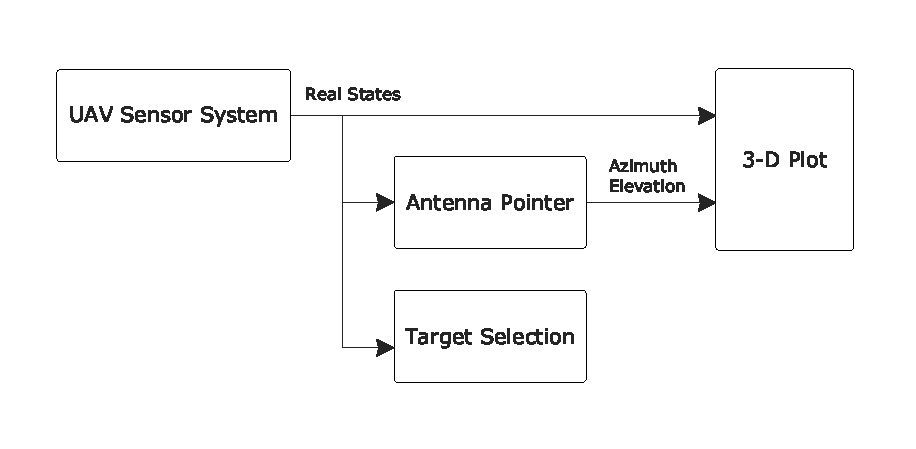
\includegraphics[scale=0.9]{./Simulink/system_overview.eps}
  \label{fig:system_overview}
  \caption[Antenna Pointer Block]{Antenna Pointer Block}
\end{figure}


\section{Antenna Pointer}
The antenna pointer block precisely points an antenna and a camera towards the aircraft. It consists of four blocks: GPS, camera, EKF/DEKF and a pointer block as shown below.
 
\begin{figure}[h!]
  %\centering
  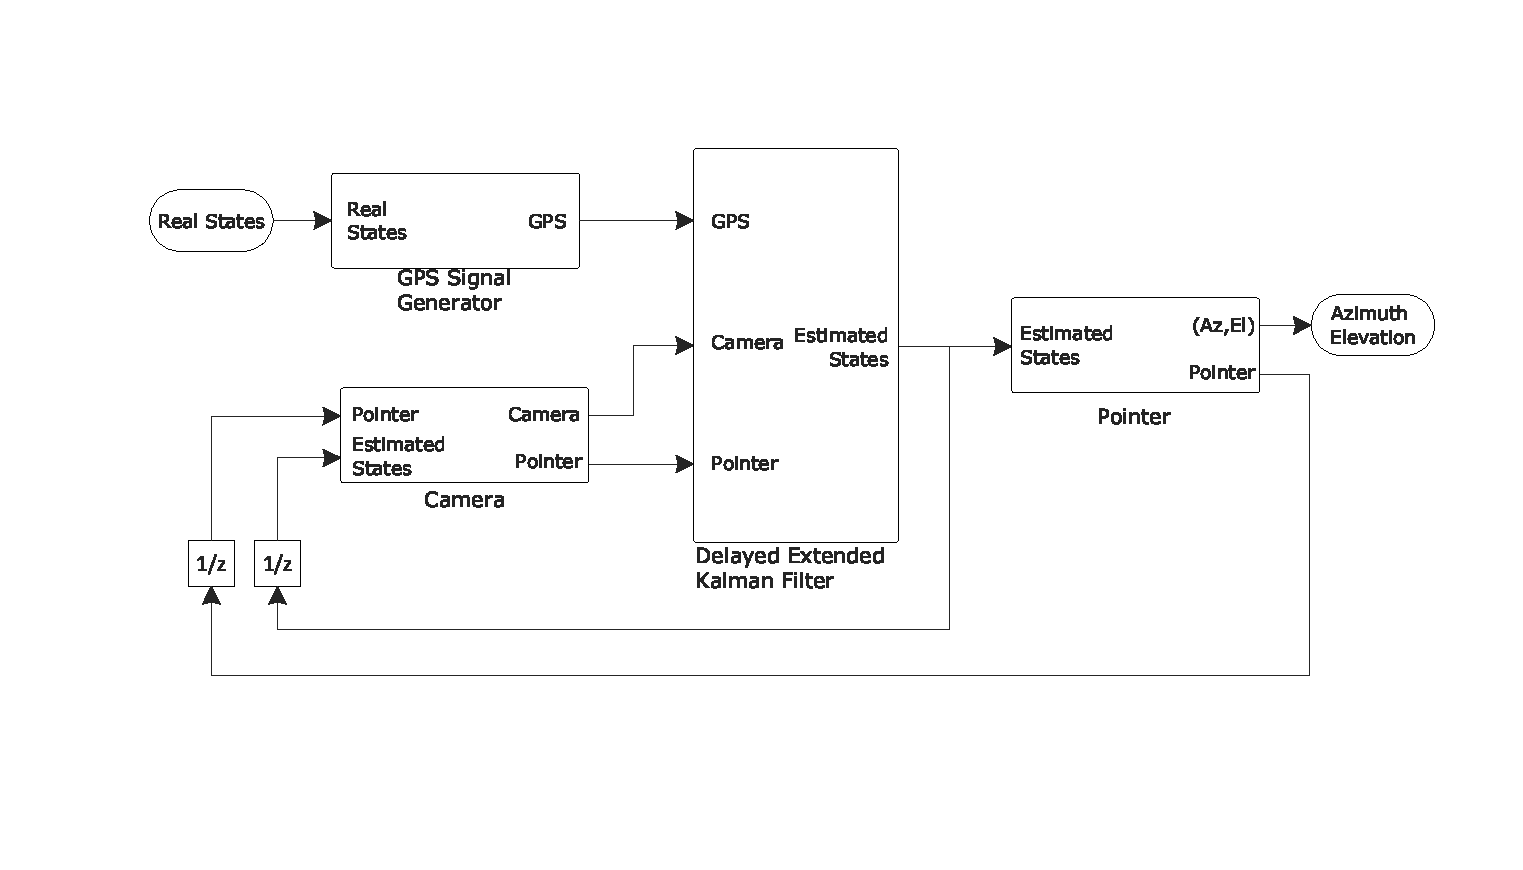
\includegraphics[scale=0.61]{./Simulink/Simulink_AP.eps}
  \label{fig:AP}
  \caption[Antenna Pointer Block]{Antenna Pointer Block. The interaction of each sub-block of the Antenna Pointer Block is shown here. The GPS receives the real measurements, adds noise and delays them. The camera receives the estimated states of the plane and if in the field of view send the position to the DEKF. The filter process all the data and outputs the estimation of the states. Finally the Pointer calculates the azimuth and elevation angles required to point towards the UAV.}
\end{figure}

\subsection{GPS}
This block generates the GPS measurements based in the real states received from the UAV sensor block. First, it reduced the frequency of the data from 100 Hz to 4 Hz, which is the common frequency found in modern GPS. Afterwards, it adds noise to the measurements as described in section \ref{sub:gps_meas_error}. Finally, it waits a random time to send each measurement to the EKF/DEKF block where they are implemented in the estimation.
\pagebreak
\subsection{Camera}
The camera block simulates a camera mounted in the antenna pointer working at 10 Hz and 20 Hz frequency. If the aircraft is in the field of view of the camera, the position in the camera frame is sent to the EKF/DEKF to introduce this data to the estimation of the states. In this simulation we assume that there is an algorithm which detects the UAV as long as it is in the field of view of the camera. The model of this camera is explained in section \ref{sub:camera_model}.

\subsection{EKF/DEKF}
This block process the information sent by the GPS and camera blocks to estimate the states of the aircraft. The processing of this data is done by the Delayed Extended Kalman filter, defined in section \ref{sub:DEKF}, which compensates for the delays in the GPS measurements. For comparison purposes the Extended Kalman filter defined in section \ref{sub:EKF} is used, to see how the estimates are impacted if we disregards the delays in the measurements.
In this work, we assume that the delays in the camera measurements can be neglected since the processing unit and the camera are connected directly.  

\subsection{Pointer}
This block calculates the angles to command and the controller of the antenna pointer. First, the pointer uses the estimated states sent by the EKF/DEKF block to calculate the azimuth and elevation angles required to point towards the aircraft. Next, the angles are sent to a simple proportional controller, defined by equations (\ref{eq:servo_commands})-(\ref{eq:servo_commands}), which actuates the servos in the antenna pointer and feedbacks the actual angles to the camera and the EKF/DEKF blocks. 
\pagebreak
\section{3-D Plot}

The purpose of this block is to collect all the data and plot the aircraft, the antenna pointer and the field of view of the camera mounted in the antenna pointer in real time.
\begin{figure}[h!]
  \centering
  \includegraphics[scale=0.7]{./Simulink/3Dplot}
  \label{fig:3dplot}
  \caption[Antenna Pointer tracking a UAV.]{Antenna Pointer tracking a UAV. This figure shows a UAV tracking different ground targets using a camera. At the same time, our antenna pointer system, follows the aircraft pointing an antenna and a camera towards it. This graphic was generated using Matlab and Simulink.}
\end{figure}
    \chapter{Results}
\label{ch:results}

This chapter presents the results gathered by the simulations explained in \ref{ch:simulation}. Three different sets of comparisons are presented. The first comparison shows the difference in accuracy of using a GPS sensor and a GPS coupled with a camera. The second case is to show how the delays affect the accuracy of the estimations. And the last case compares the estimations of the Extended Kalman filter against the Delayed Extended Kalman filter with delayed measurements, to see the impact of disregarding the delays.

\section{Comparison of Estimations Between GPS and GPS Coupled with Camera}
In this scenario, we focus on the comparison between using a GPS at 1 Hz coupled with a camera at 20 Hz, and the GPS alone. The introduction of the camera measurements are expected to improve the estimation. In this case, the GPS measurements have a random delay of 0.75 seconds.
%The first case uses one GPS sensor in the UAS with a frequency of 4 Hz. The measurement is assumed to be received instantaneously. This situation is not real but it is going to be simulated for the purpose of comparison and to recognize the impact that delays have in the estimates.
\begin{figure}[H]
  \centering
  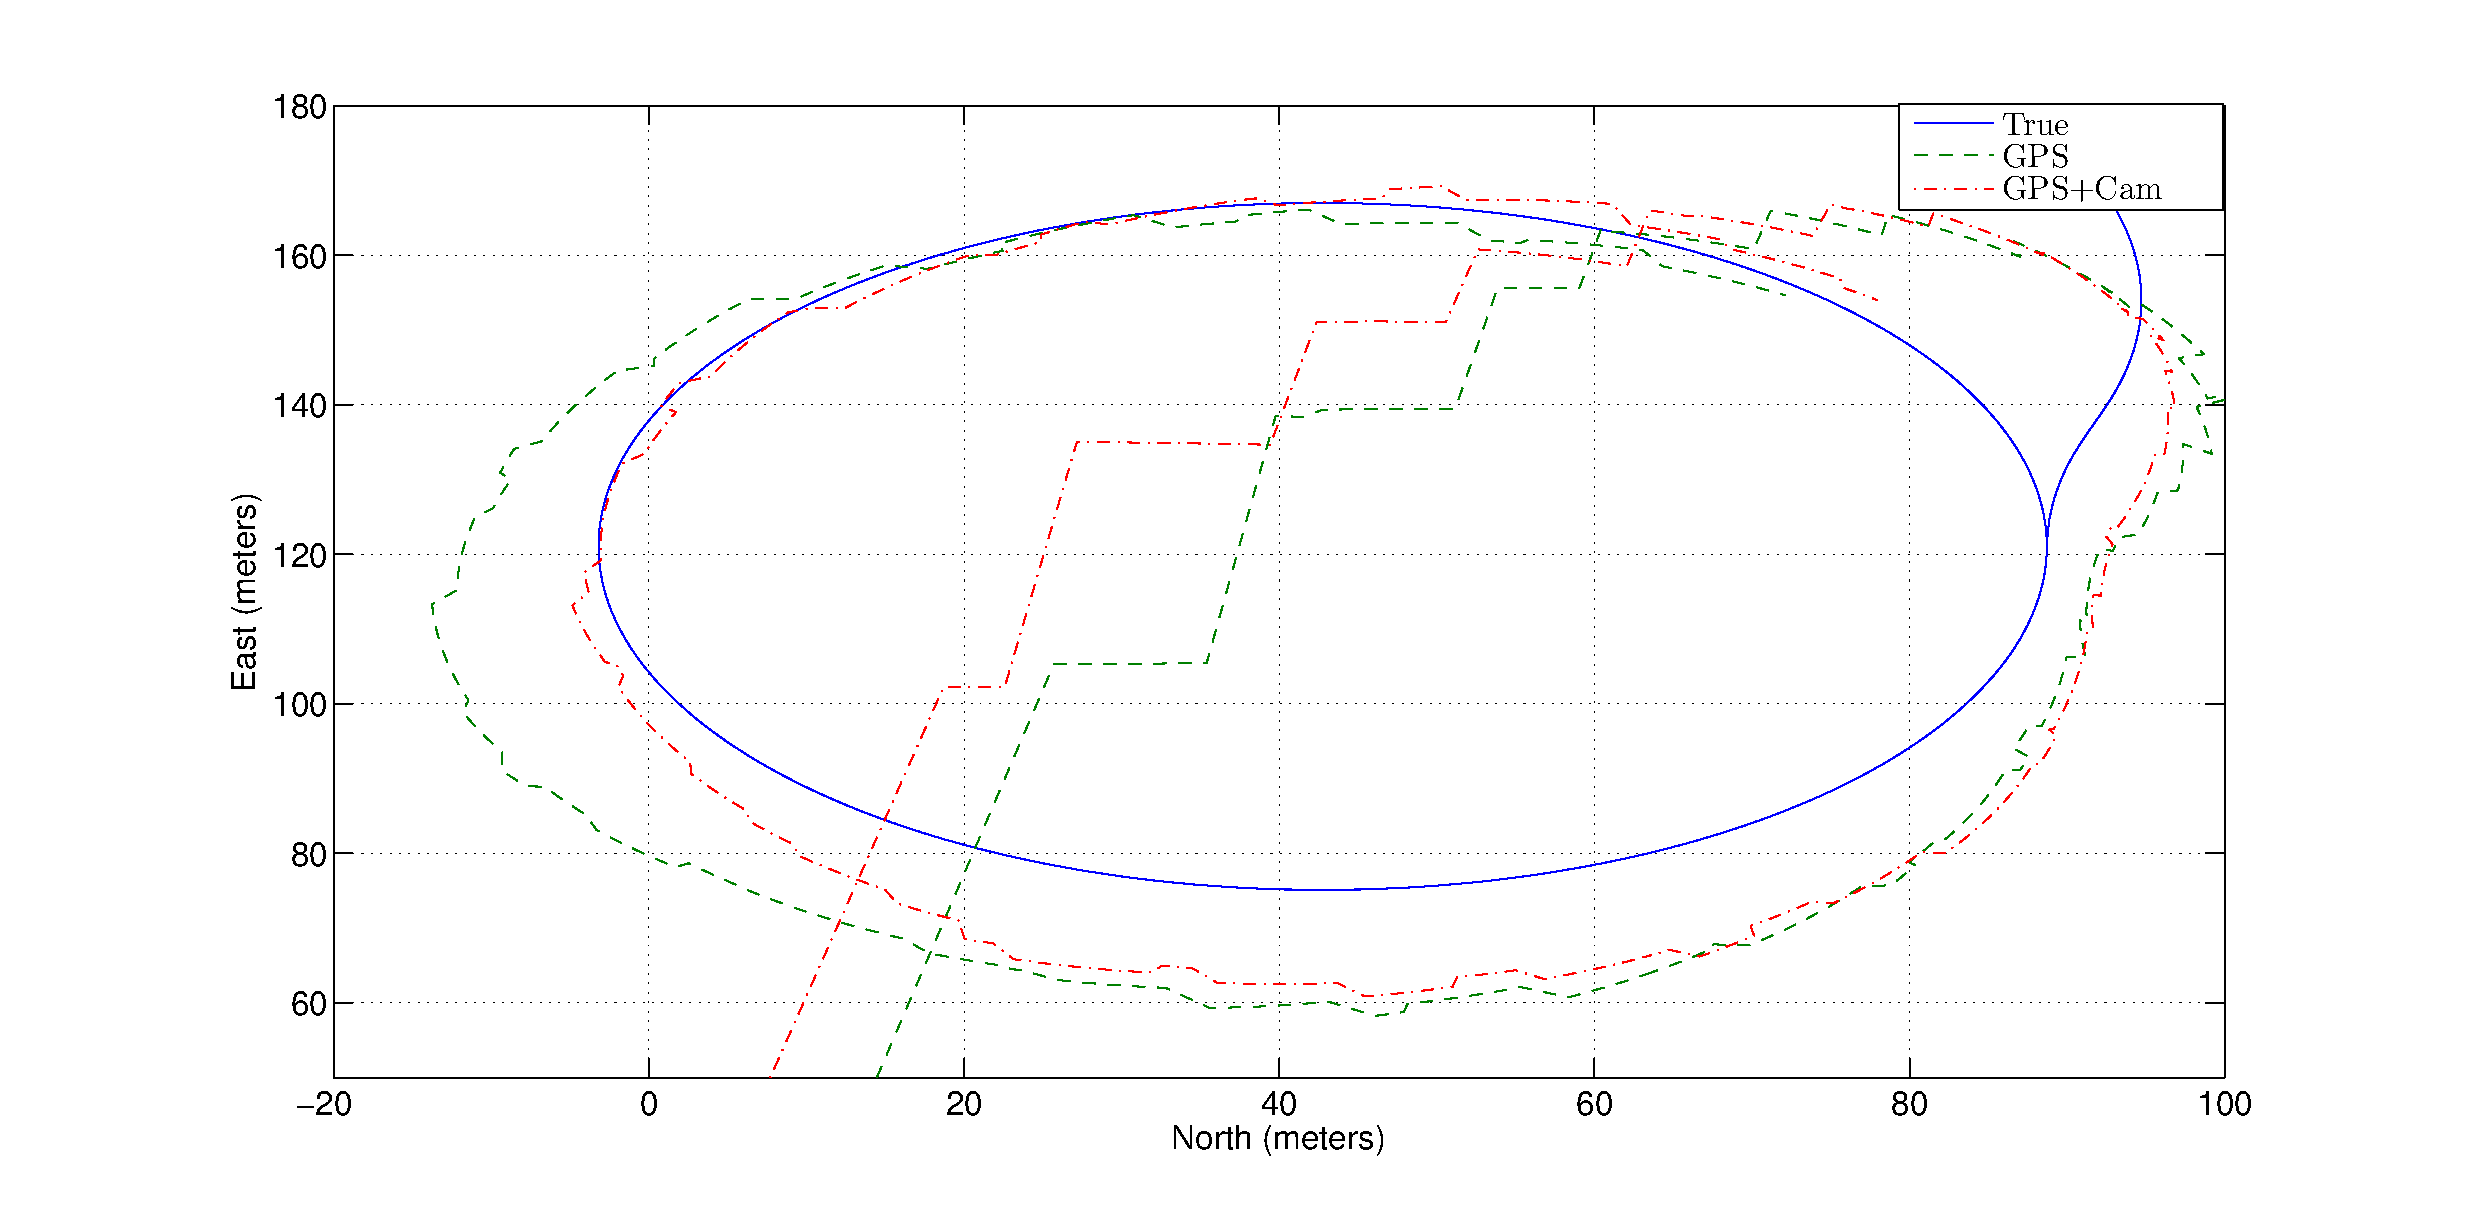
\includegraphics[scale=0.40]{./Results/GPS_vs_GPS+Cam/uav_trajectory.eps}
  \caption[UAV Trajectory Comparison - GPS vs GPS and Camera]{UAV Trajectory Comparison - GPS vs GPS and Camera. The real trajectory of the aircraft is shown in this plot, against the estimated trajectory calculated by using a GPS coupled with a camera, and just a GPS.}
\end{figure}

\begin{figure}[H]
  \centering
  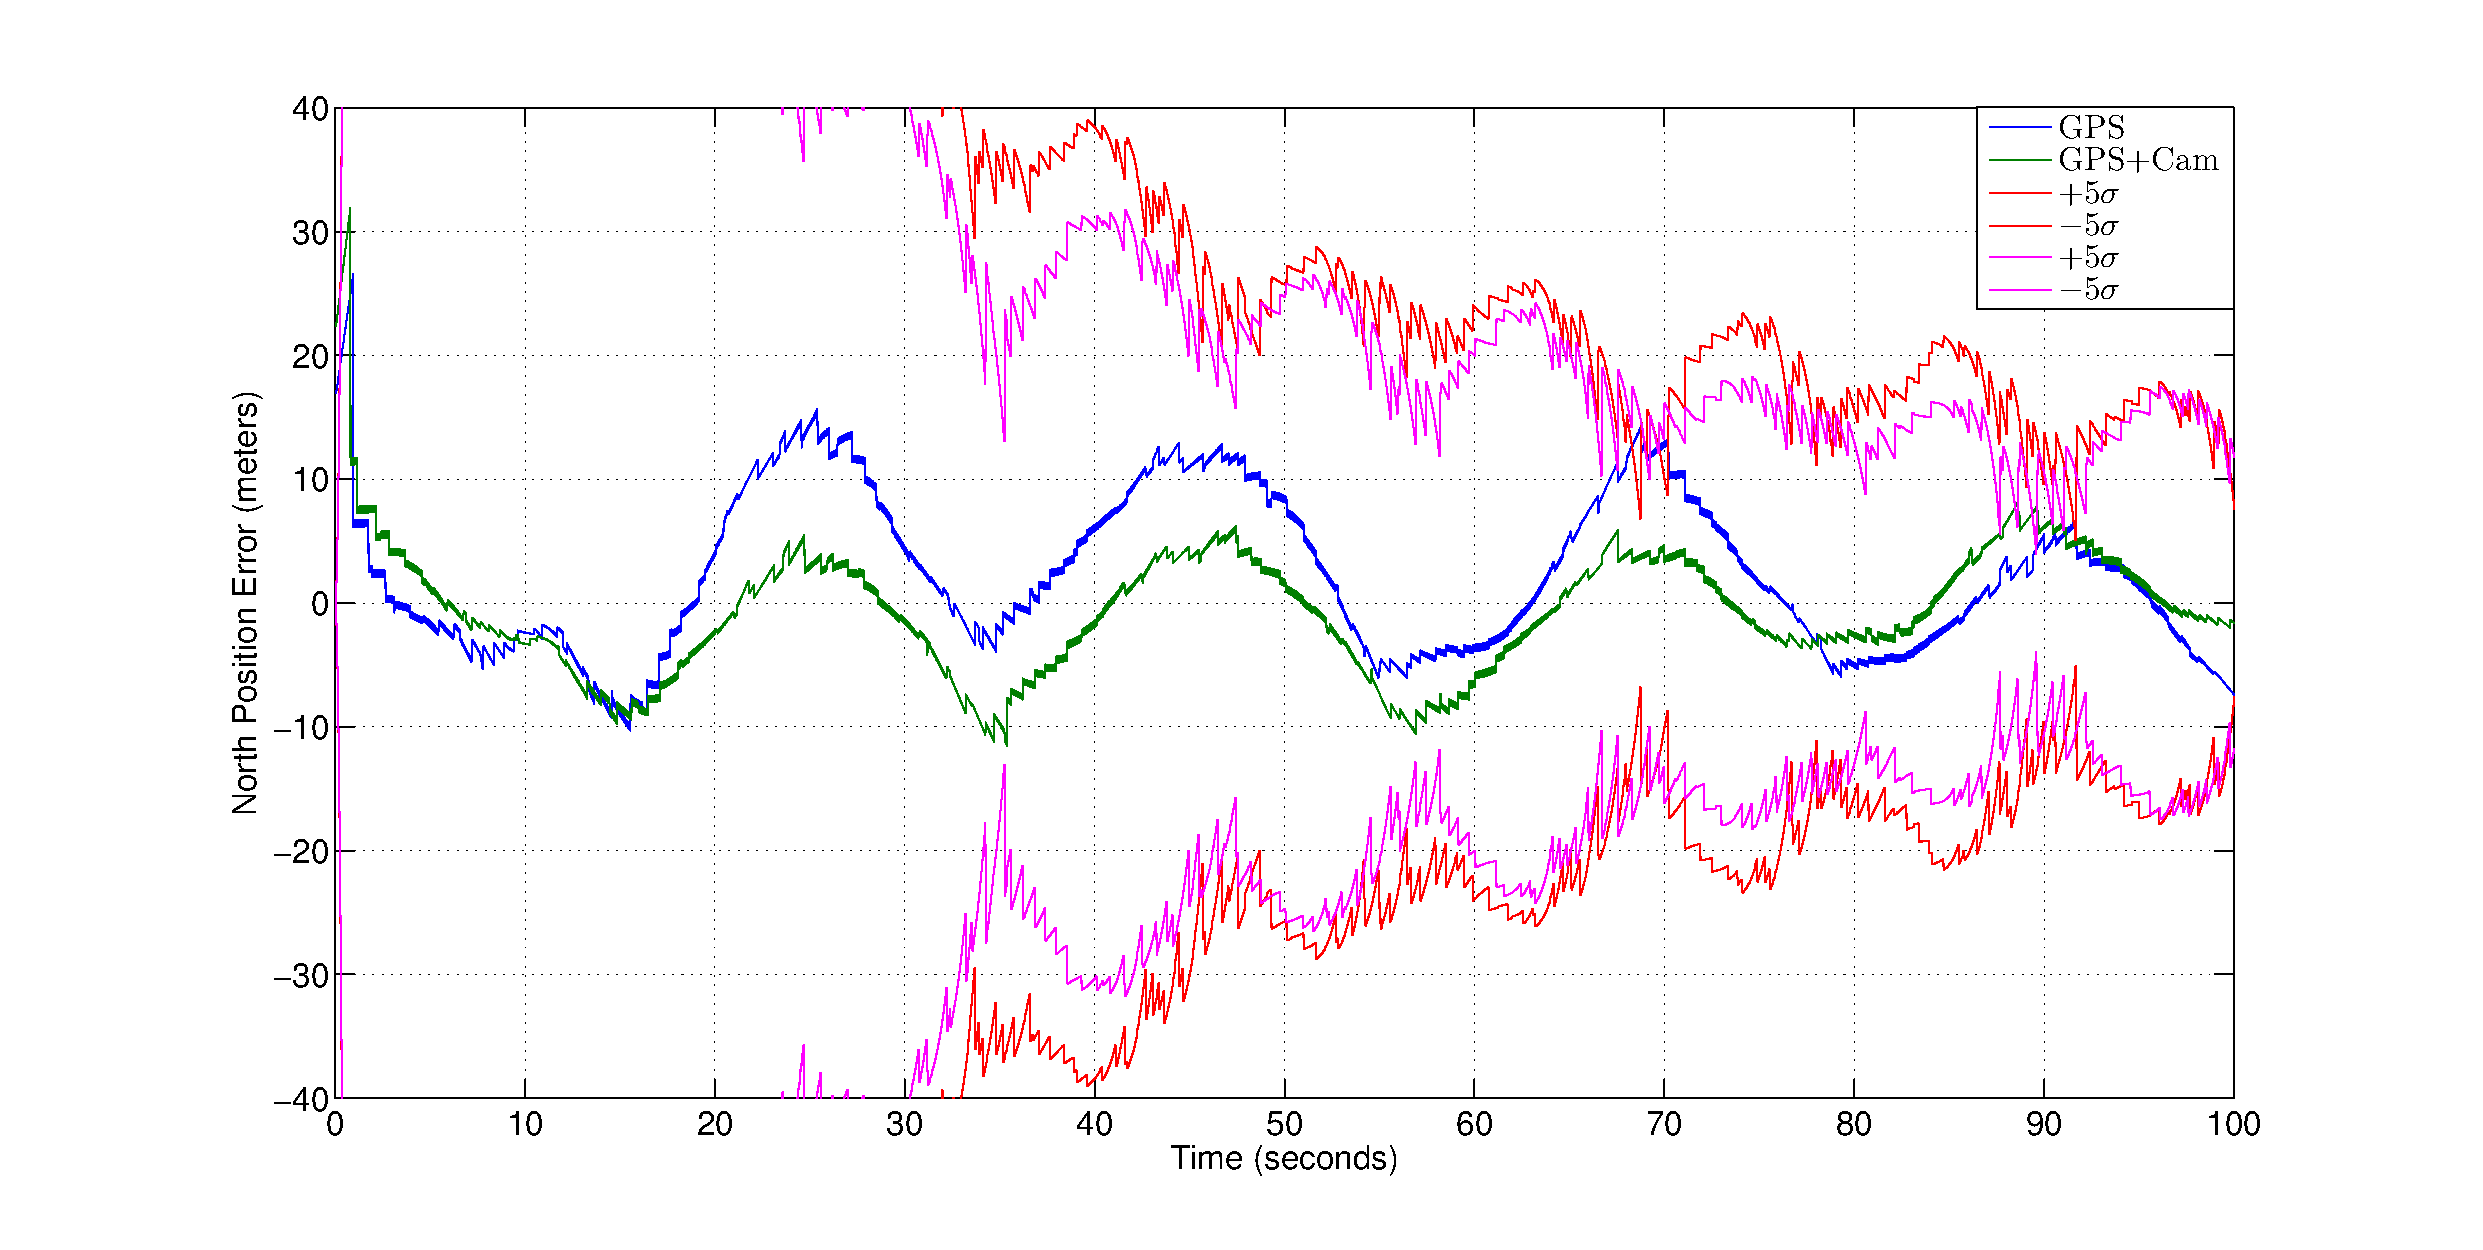
\includegraphics[scale=0.40]{./Results/GPS_vs_GPS+Cam/north_comparison.eps}
  \caption[North Position Error Comparison - GPS vs GPS and Camera]{North Position Error Comparison - GPS vs GPS and Camera. The error in the north position is shown in this plot. The states estimations are compared for GPS and GPS coupled with a camera.}
\end{figure}

\begin{figure}[H]
  \centering
  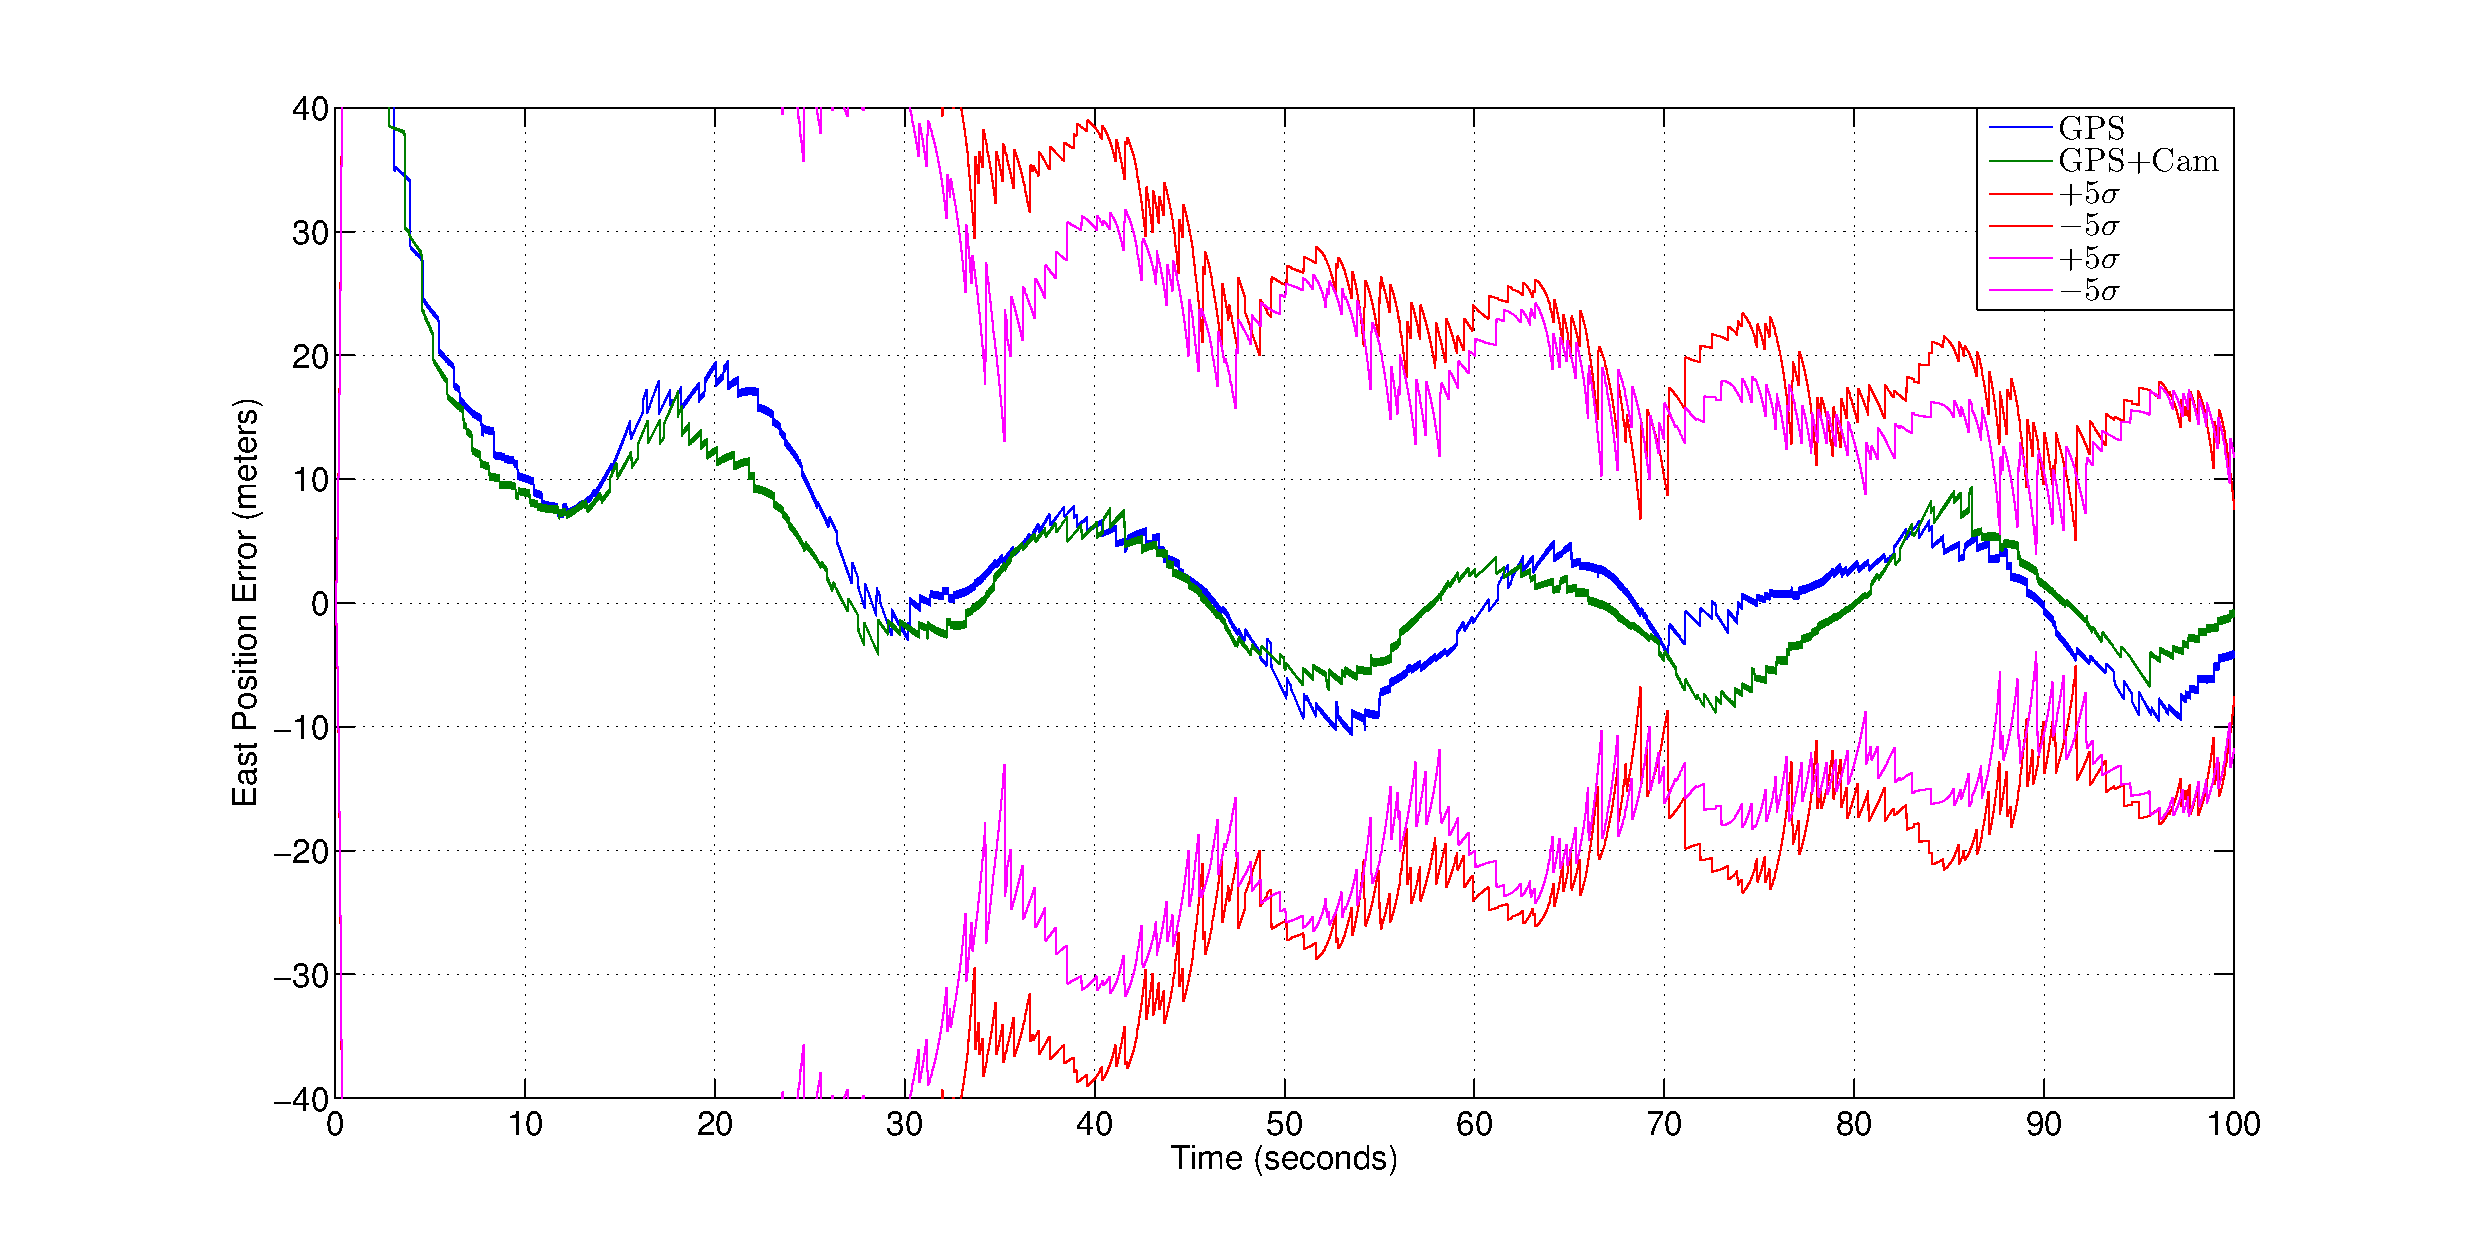
\includegraphics[scale=0.40]{./Results/GPS_vs_GPS+Cam/east_comparison.eps}
  \caption[East Position Error Comparison - GPS vs GPS and Camera]{East Position Error Comparison - GPS vs GPS and Camera. The error in the east position is shown in this plot. The states estimations are compared for GPS and GPS coupled with a camera.}
\end{figure}

\begin{figure}[H]
  \centering
  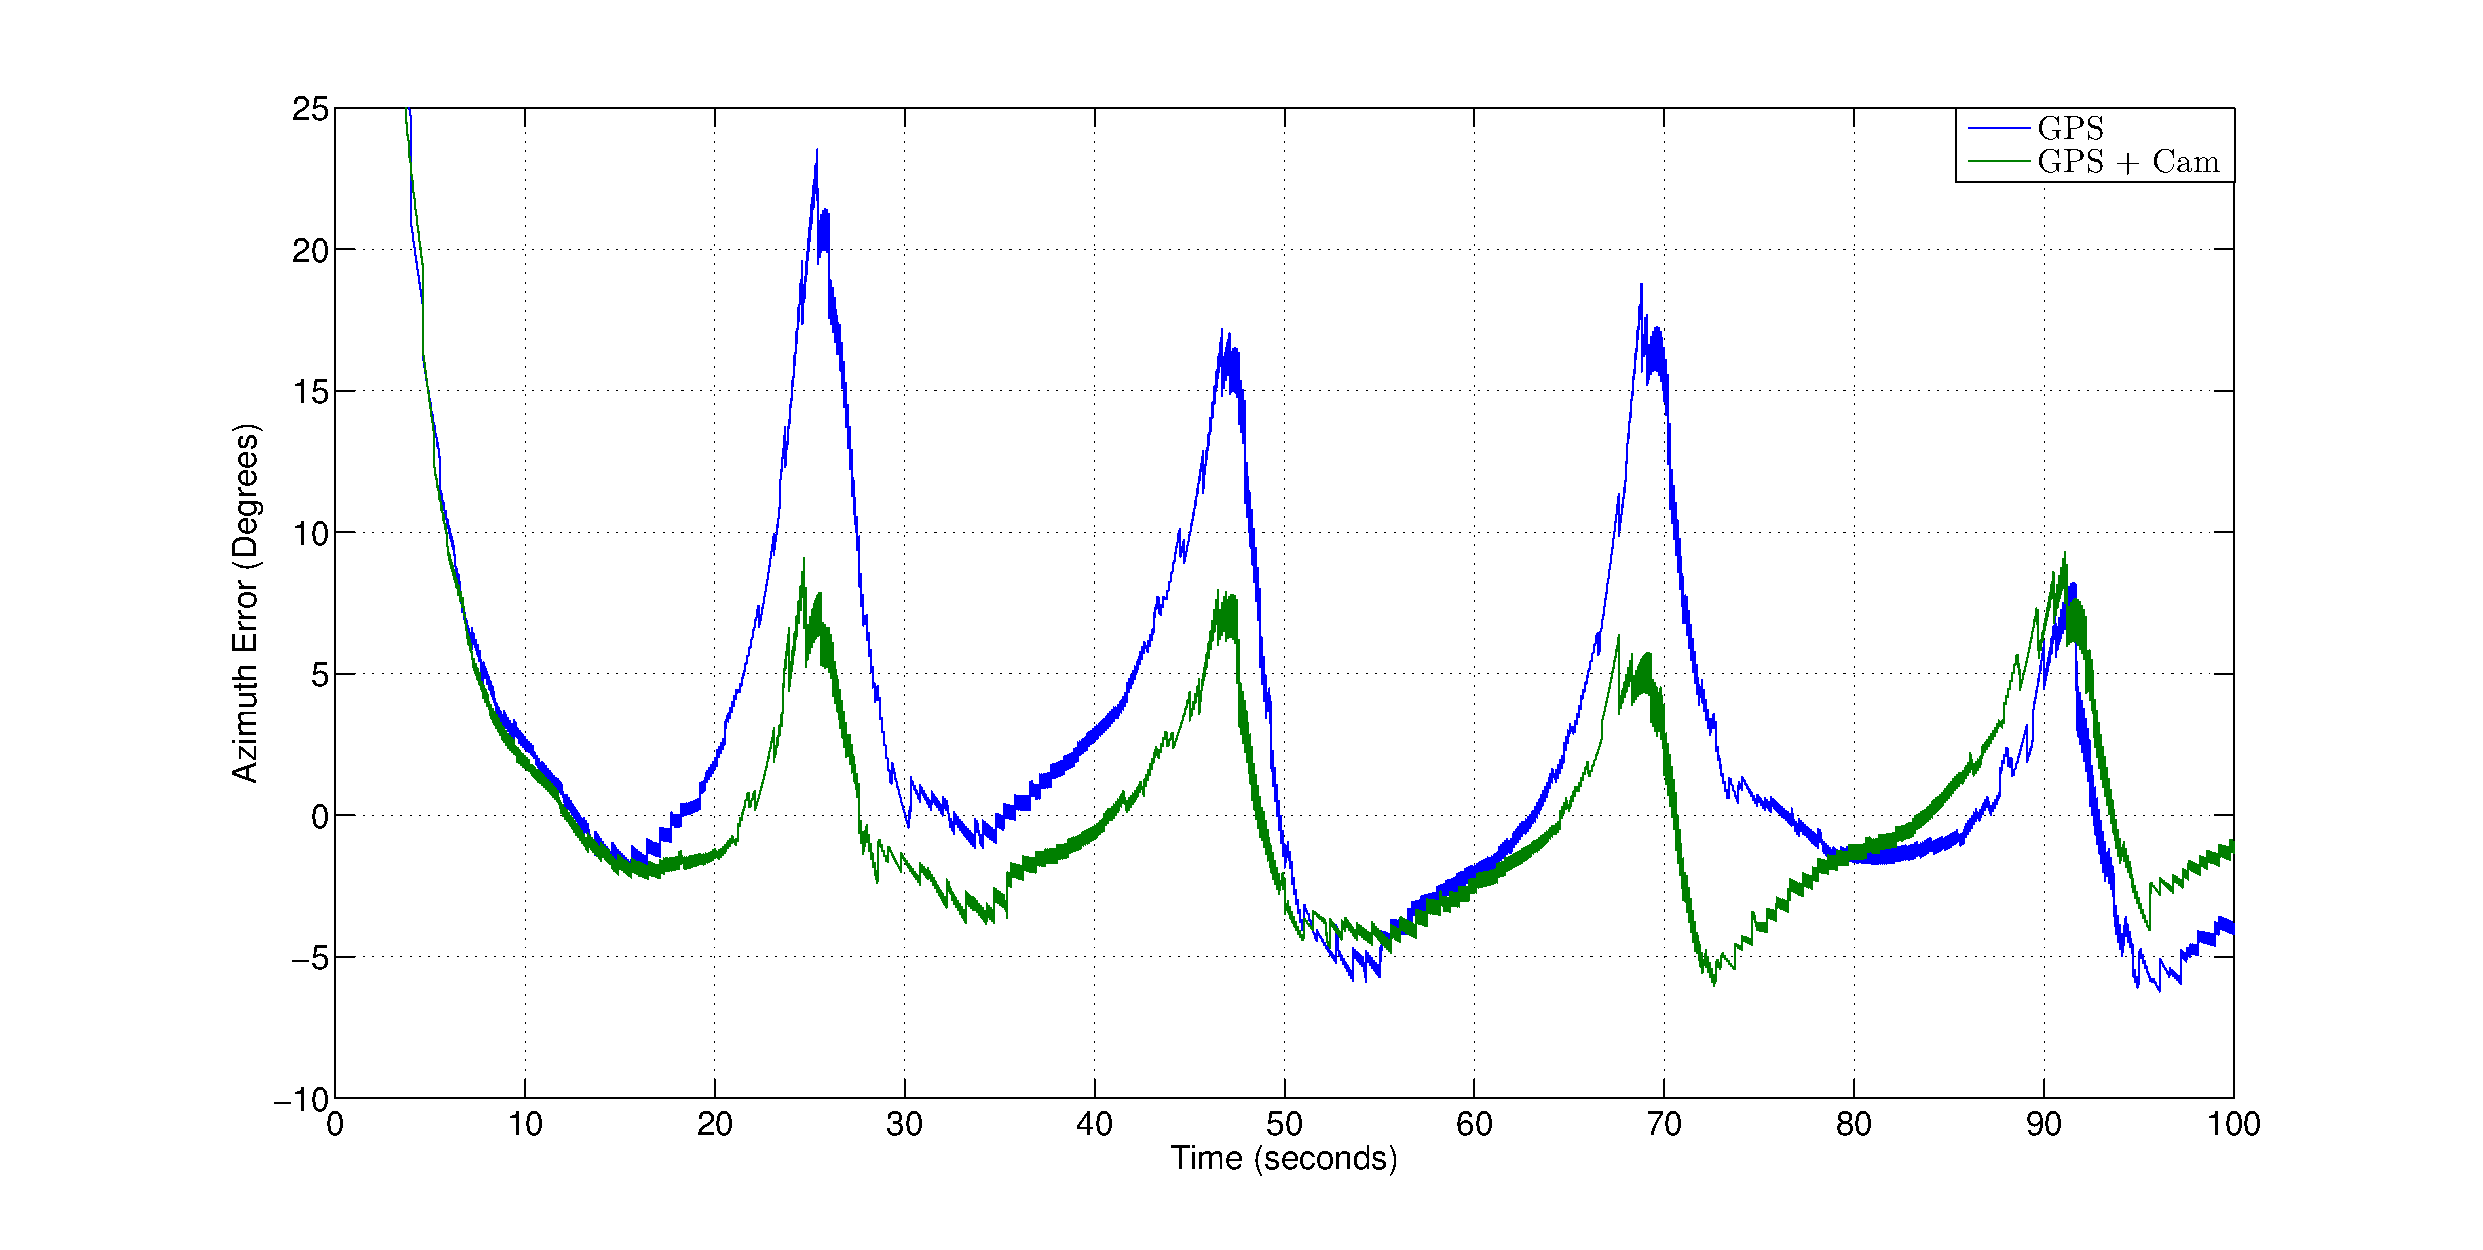
\includegraphics[scale=0.40]{./Results/GPS_vs_GPS+Cam/azimuth_comparison.eps}
  \caption[Azimuth Error Comparison - GPS vs GPS coupled with Camera]{Azimuth Error Comparison - GPS vs GPS coupled with Camera. The error in the azimuth angle calculated by the estimations are presented. It can be seen that coupling a GPS with a camera improves the estimation.}
\end{figure}
\begin{figure}[H]
  \centering
  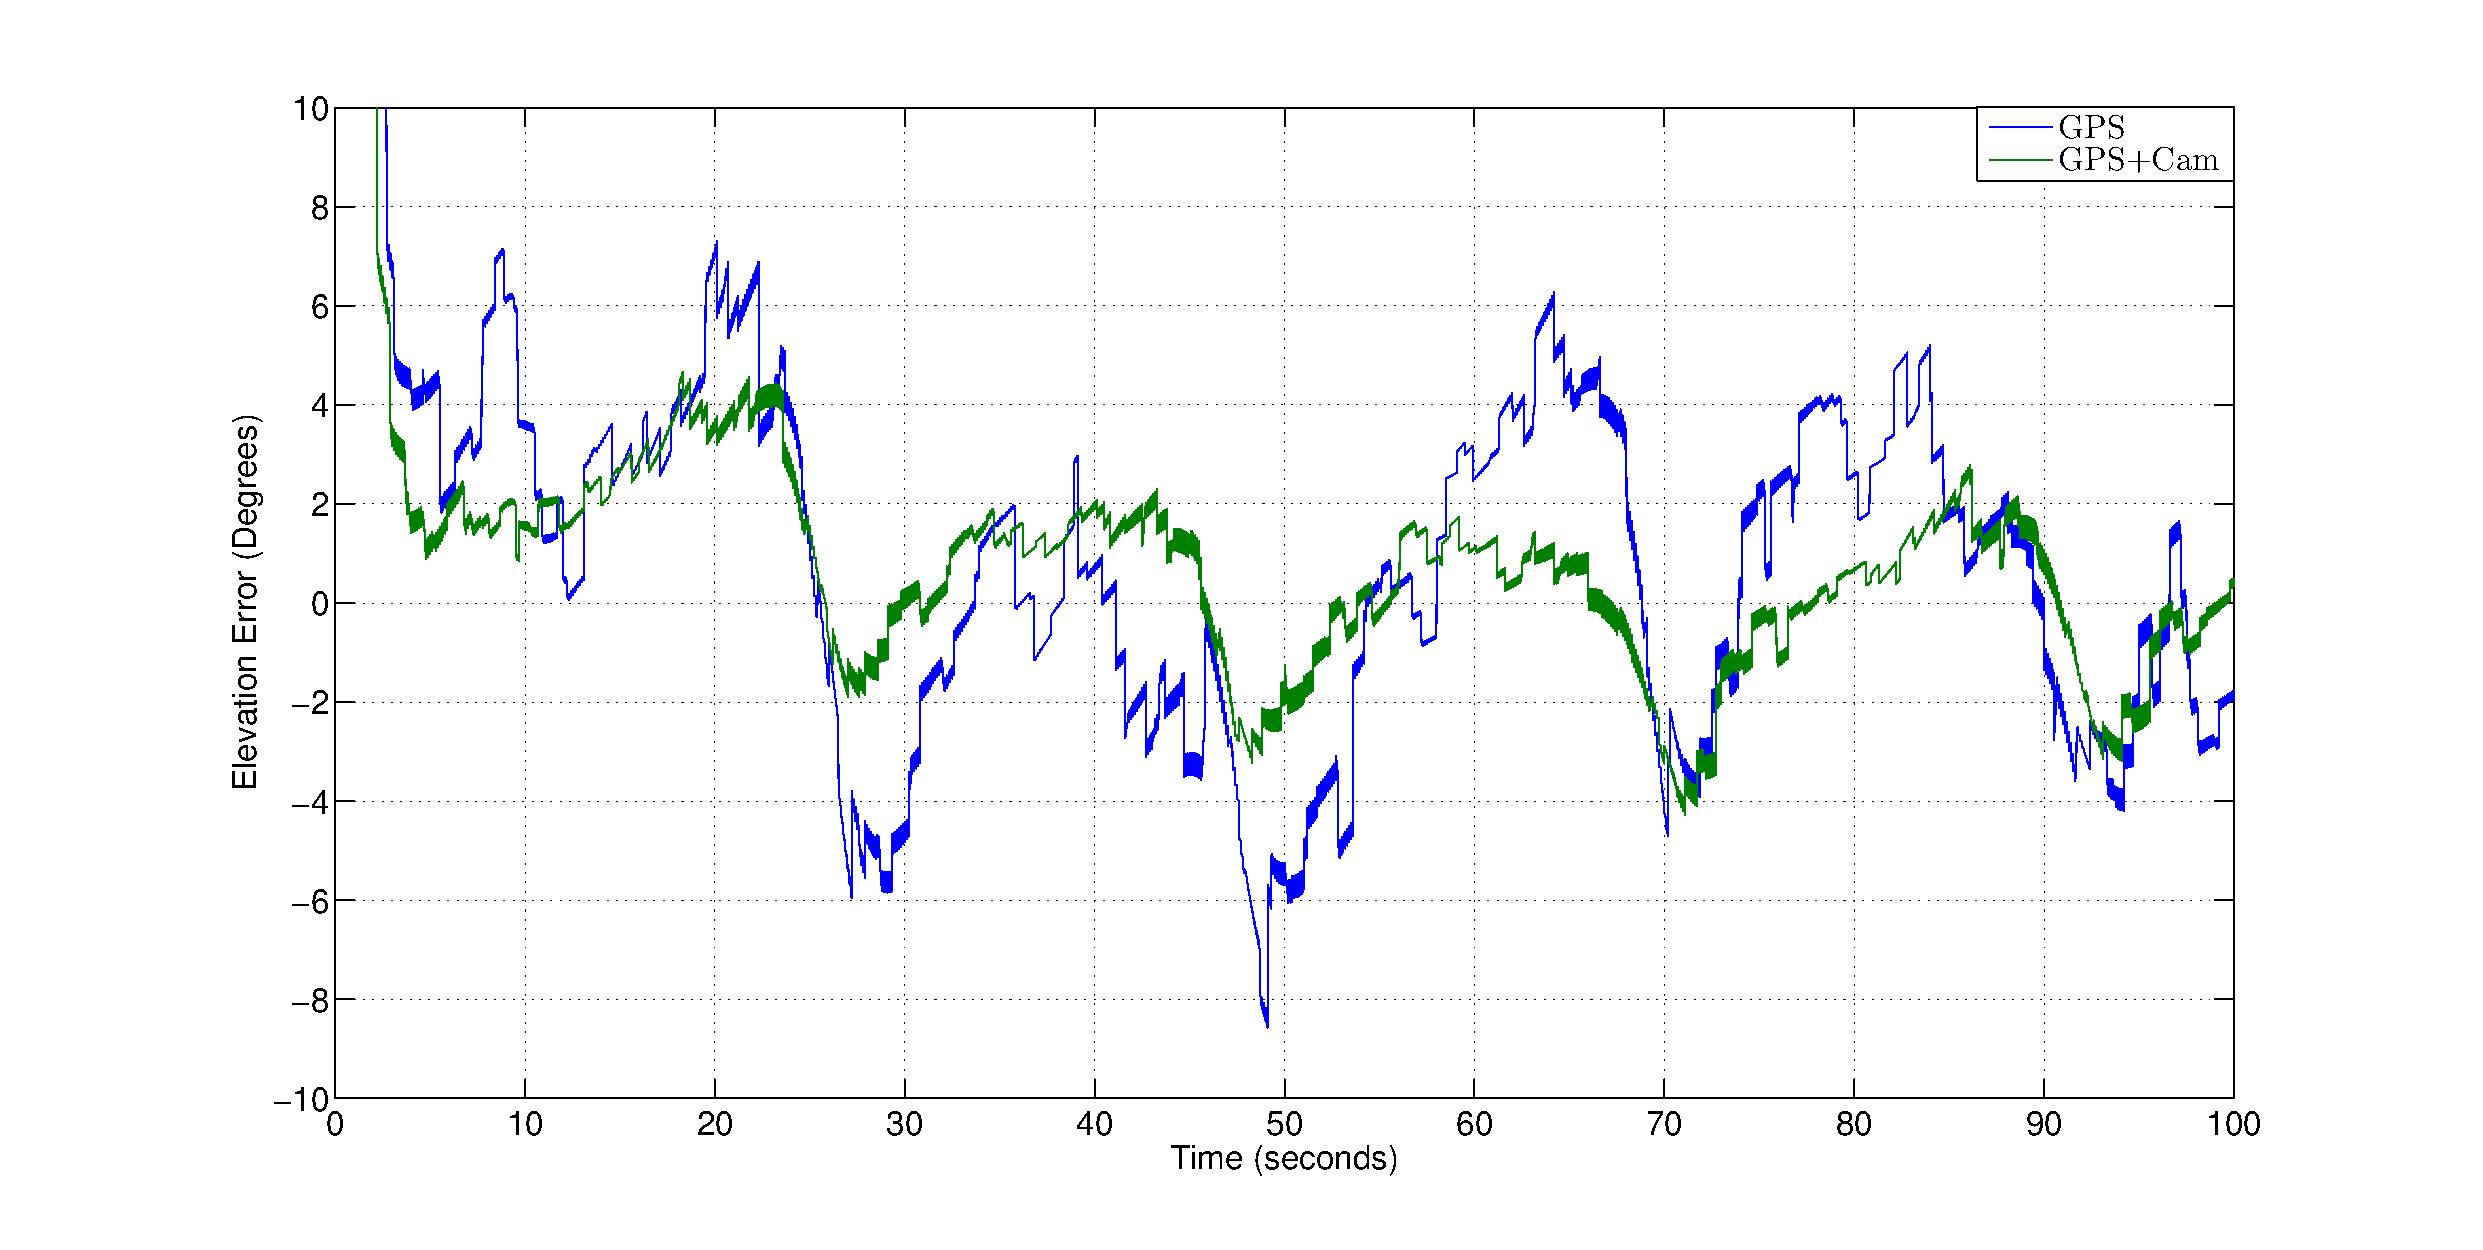
\includegraphics[scale=0.40]{./Results/GPS_vs_GPS+Cam/elevation_comparison.eps}
  \caption[Elevation Error Comparison - GPS vs GPS coupled with Camera]{Elevation Error Comparison - GPS vs GPS coupled with Camera. The error in the elevation angle calculated by the estimations are presented. It can be seen that coupling a GPS with a camera improves the estimation.}
\end{figure}

\pagebreak

\section{Comparison of Estimation Accuracy for EKF and DEKF with 0.75 s Random Delay}
In this scenario the precision of the state estimations from an EKF and a DEKF are considered. Again, a GPS coupled with a camera serves as the inputs for the filters. Here we show how the estimations are impacted if the measurements have delays and a filter that does not take them into account is used. An improvement in the estimations is expected using the DEKF.

\begin{figure}[H]
  \centering
  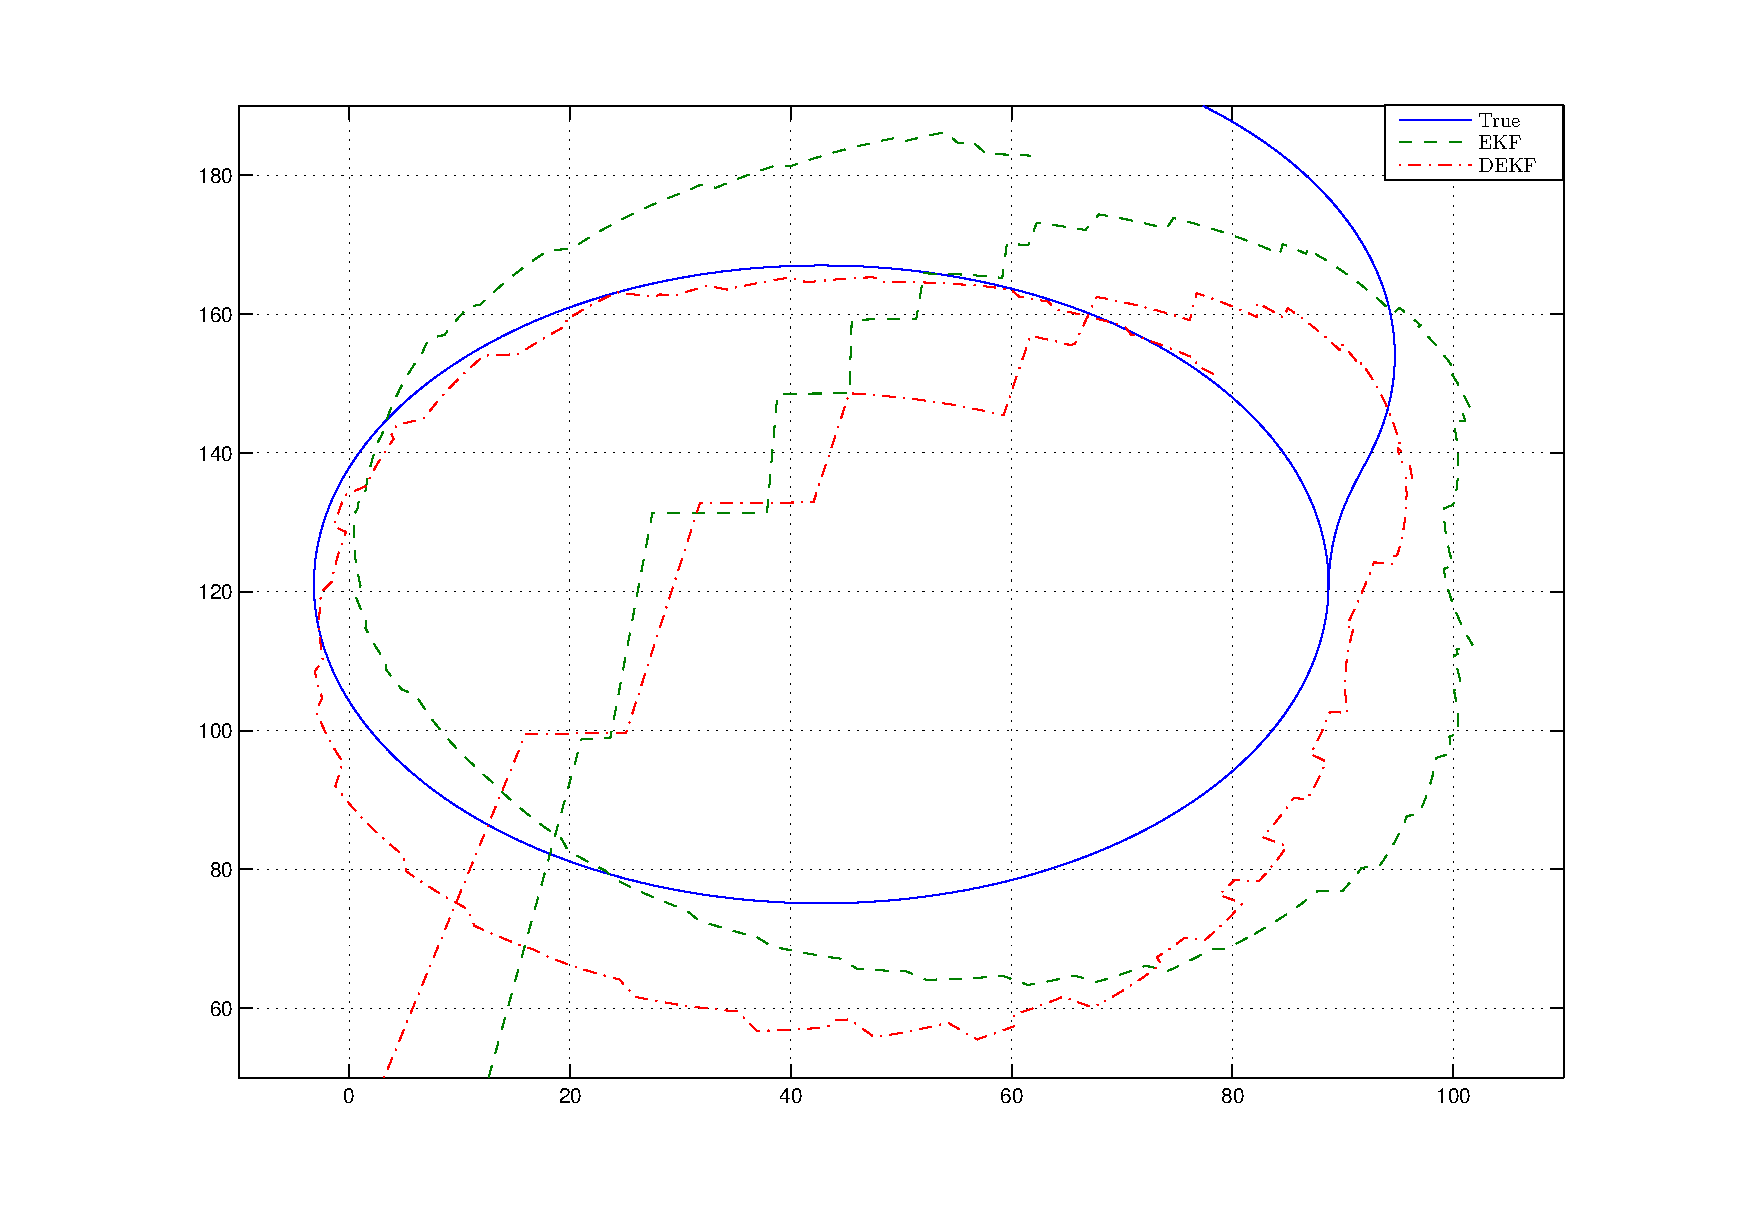
\includegraphics[scale=0.55]{./Results/EKF_vs_DEKF/uav_trajectory.eps}
  \caption[UAV Trajectory Comparison - EKF vs DEKF]{UAV Trajectory Comparison - EKF vs DEKF. The trajectory of the aircraft is shown in this plot, against the estimated trajectory calculated by an EKF and by a DEKF.}
\end{figure}

\begin{figure}[H]
  \centering
  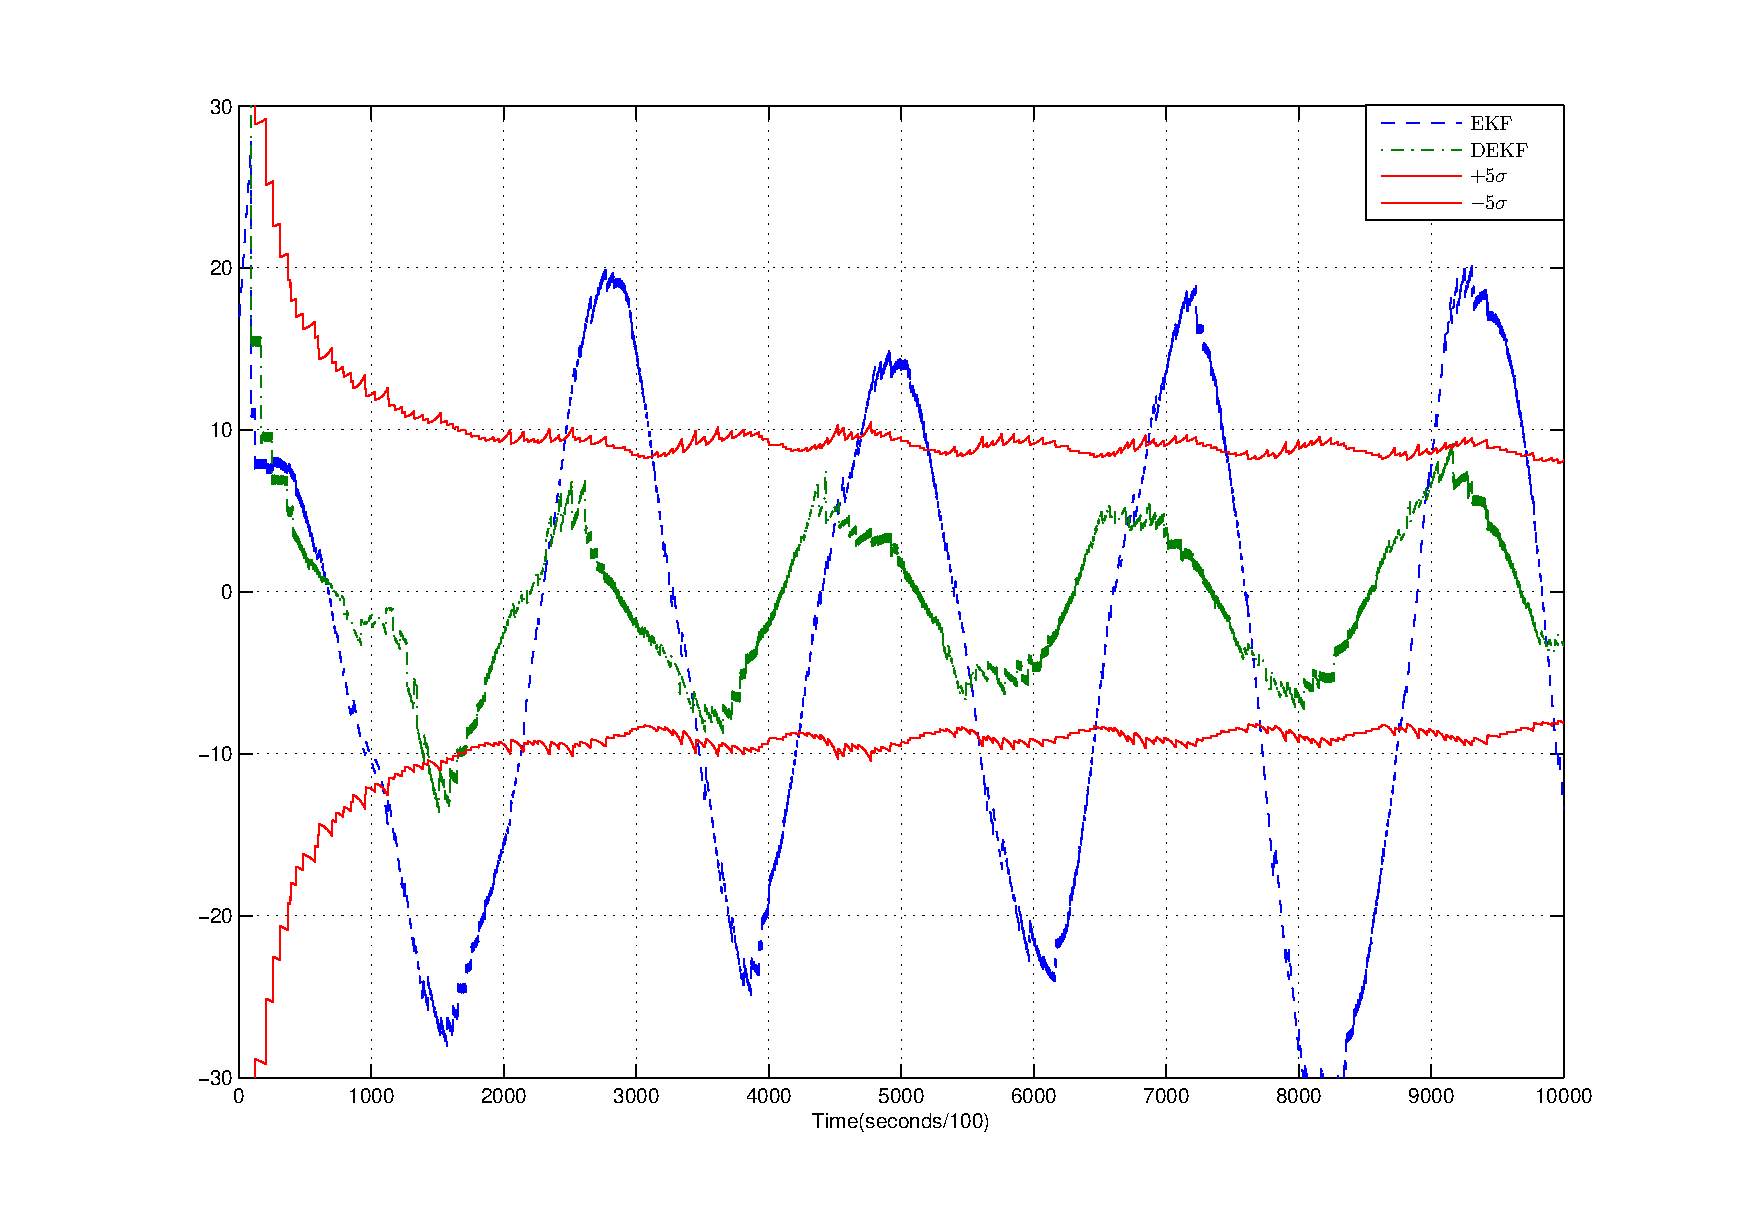
\includegraphics[scale=0.40]{./Results/EKF_vs_DEKF/north_error_comparison.eps}
  \caption[North Position Error Comparison - EKF vs DEKF]{North Position Error Comparison - EKF vs DEKF. The error in the north position is shown in this plot. The states estimations are compared for an EKF and a DEKF.}
\end{figure}

\begin{figure}[H]
  \centering
  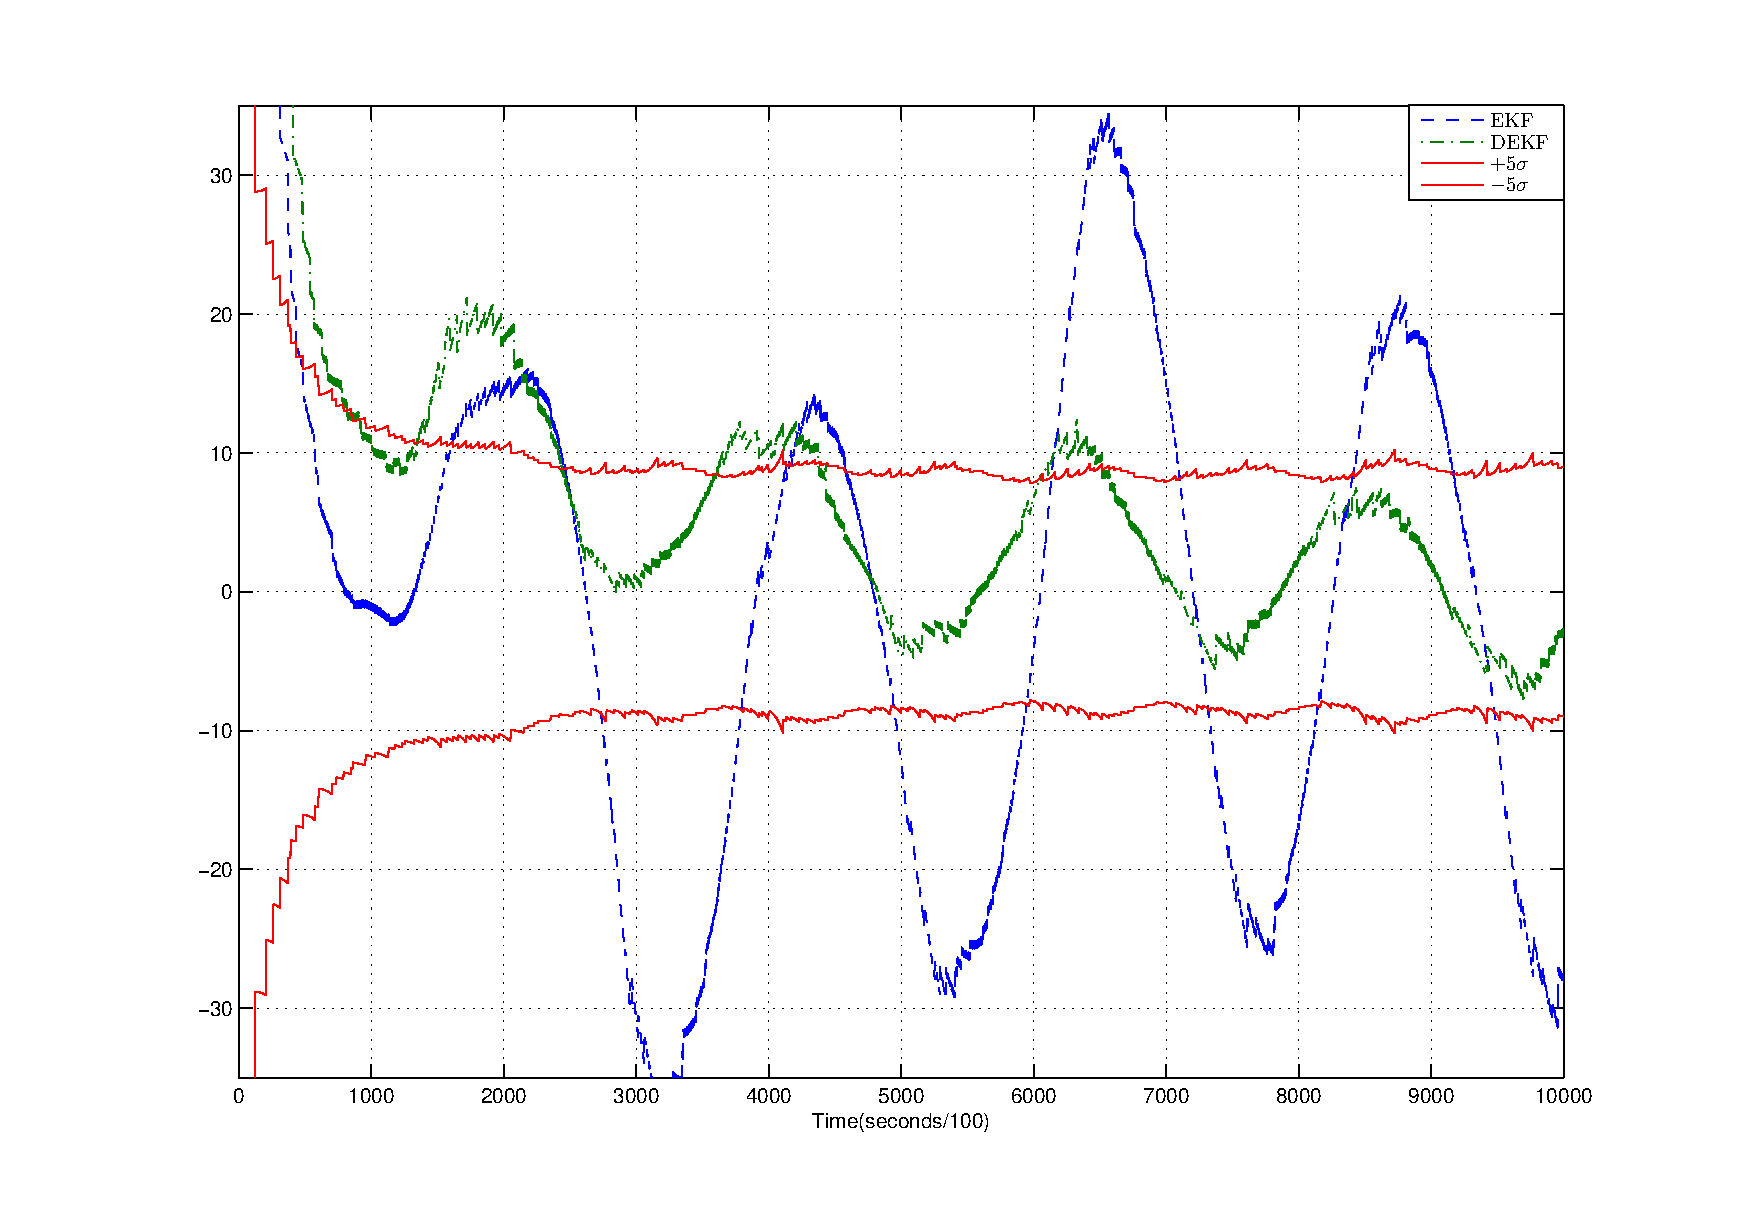
\includegraphics[scale=0.40]{./Results/EKF_vs_DEKF/east_error_comparison.eps}
  \caption[East Position Error Comparison - EKF vs DEKF]{East Position Error Comparison - EKF vs DEKF. The error in the east position is shown in this plot. The states estimations are compared for an EKF and a DEKF.}
\end{figure}

\begin{figure}[H]
  \centering
  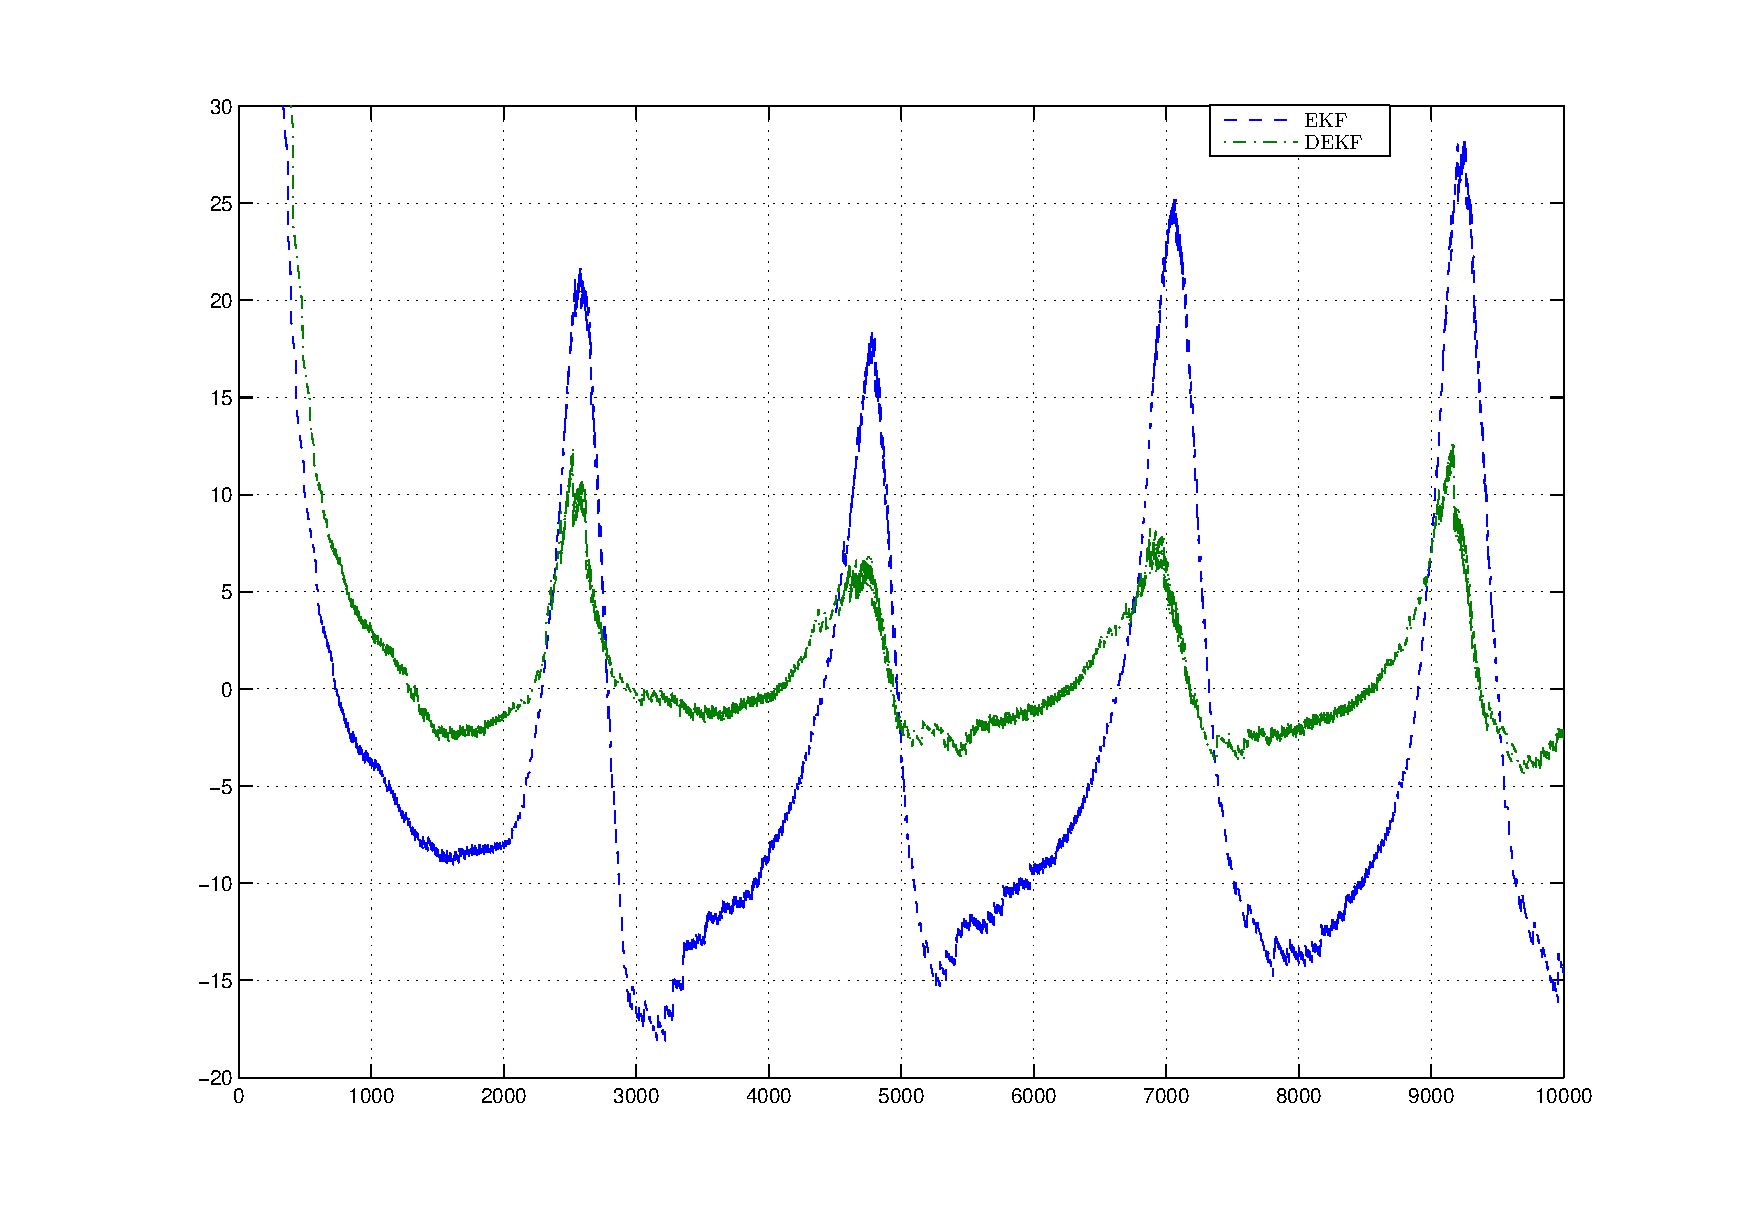
\includegraphics[scale=0.40]{./Results/EKF_vs_DEKF/azimuth_error_comparison.eps}
  \caption[Azimuth Error Comparison - EKF vs DEKF]{Azimuth Error Comparison - EKF vs DEKF. The error in the azimuth angle calculated by the estimations is shown in this plot. Azimuth for the EKF and the DEKF are compared.}
\end{figure}

\begin{figure}[H]
  \centering
  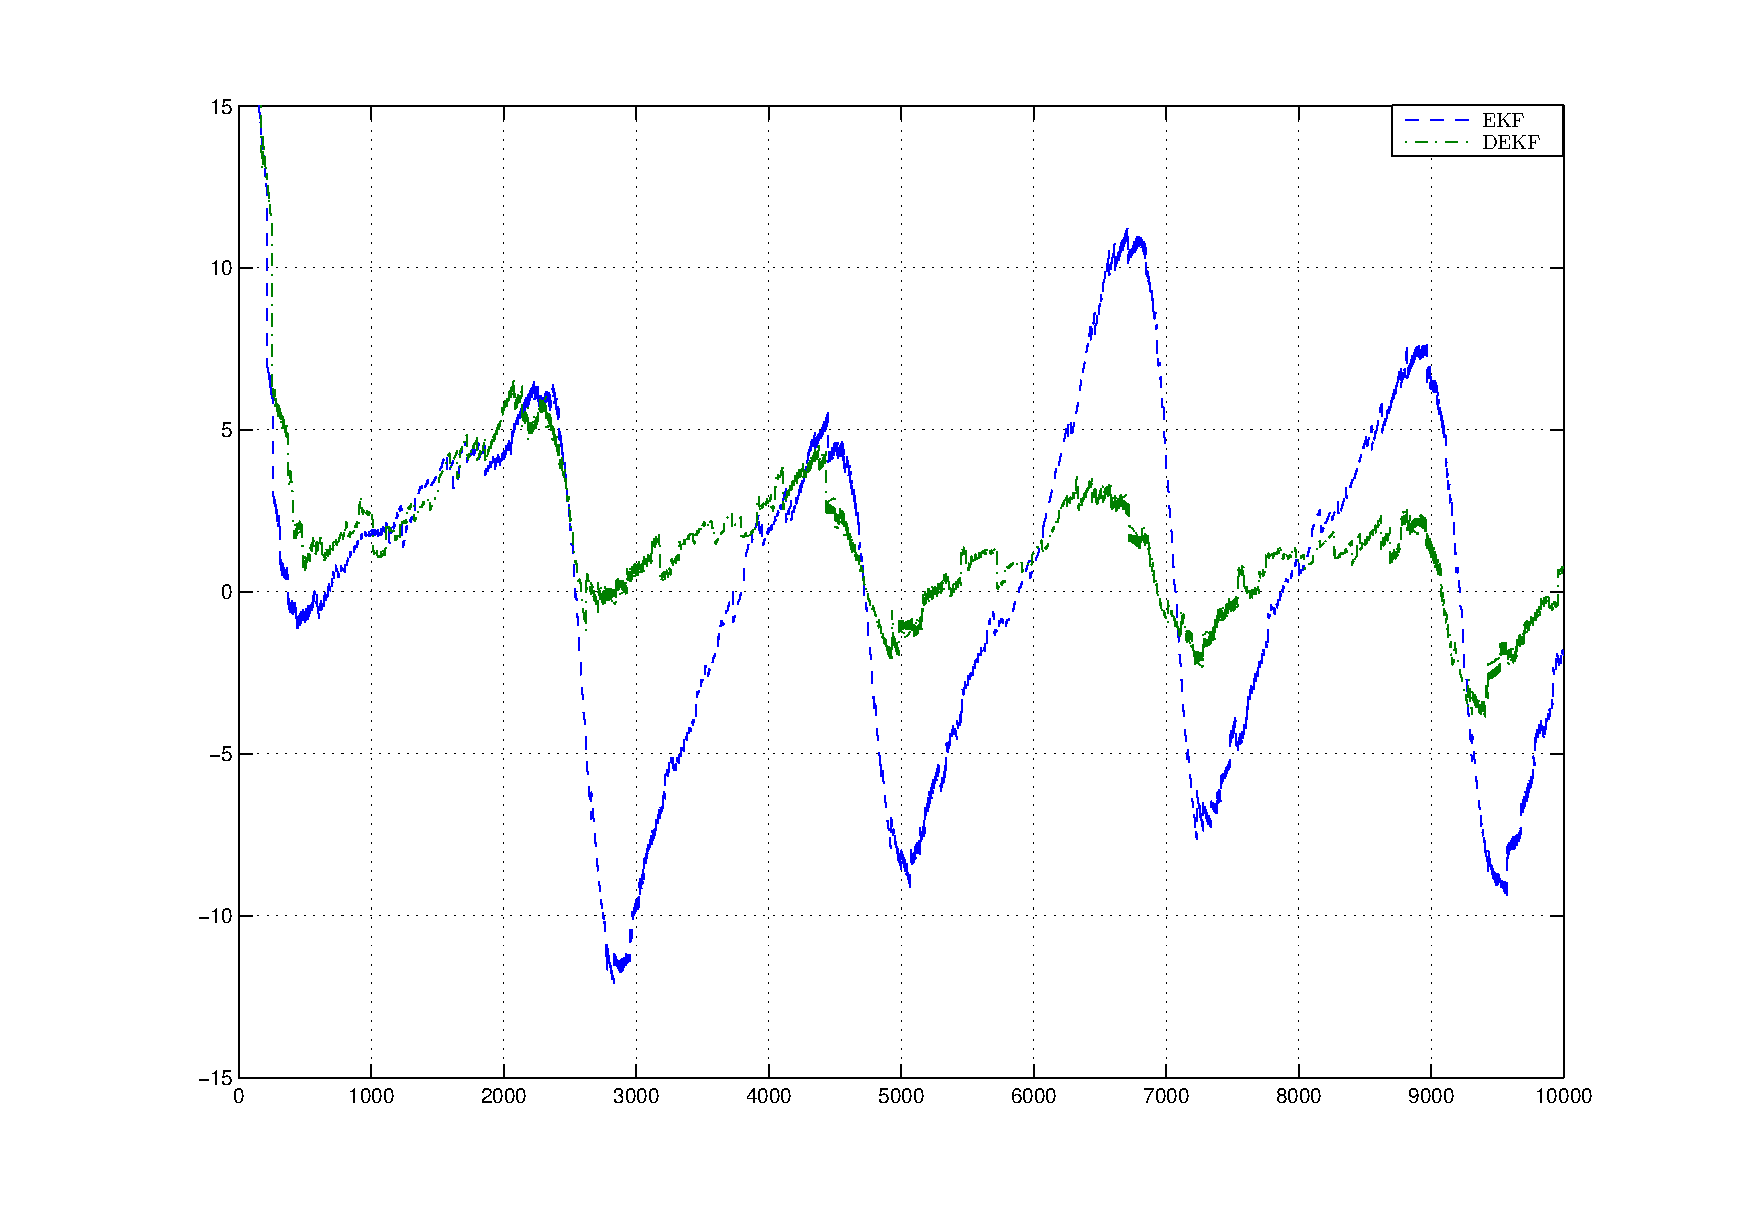
\includegraphics[scale=0.40]{./Results/EKF_vs_DEKF/elevation_error_comparison.eps}
  \caption[Elevation Error Comparison - EKF vs DEKF]{Elevation Error Comparison - EKF vs DEKF. The error in the elevation angle calculated by the estimations is shown in this plot. Elevation for the EKF and the DEKF are compared.}
\end{figure}

\section{Comparison of Estimation Accuracy Between No delay, 0.25 s, 0.50 s, and 0.75 s Random Delays}
For this scenario we will use a GPS coupled with a camera. This scenario compares the estimation made by a DEKF for no delay, random delay of up to 0.25 s, 0.50 s, and 0.75 s. Since the delays are randomly generated, some of the measurements arrive in an out-of-sequence fashion. The Delayed Extended Kalman filter also compensates for this.

%This configuration uses a GPS sensor at 4 Hz coupled with a camera at 10 Hz. As explained before, the reason for this configuration comes from the nature of each sensor. The GPS has relative low error at medium and long distance but not at close range. Inversely, the camera is faster than the GPS and makes good estimations at short distances, but at medium and long range it can not detect the target. Hence, the sensors complement each other.

\begin{figure}[H]
  \centering
  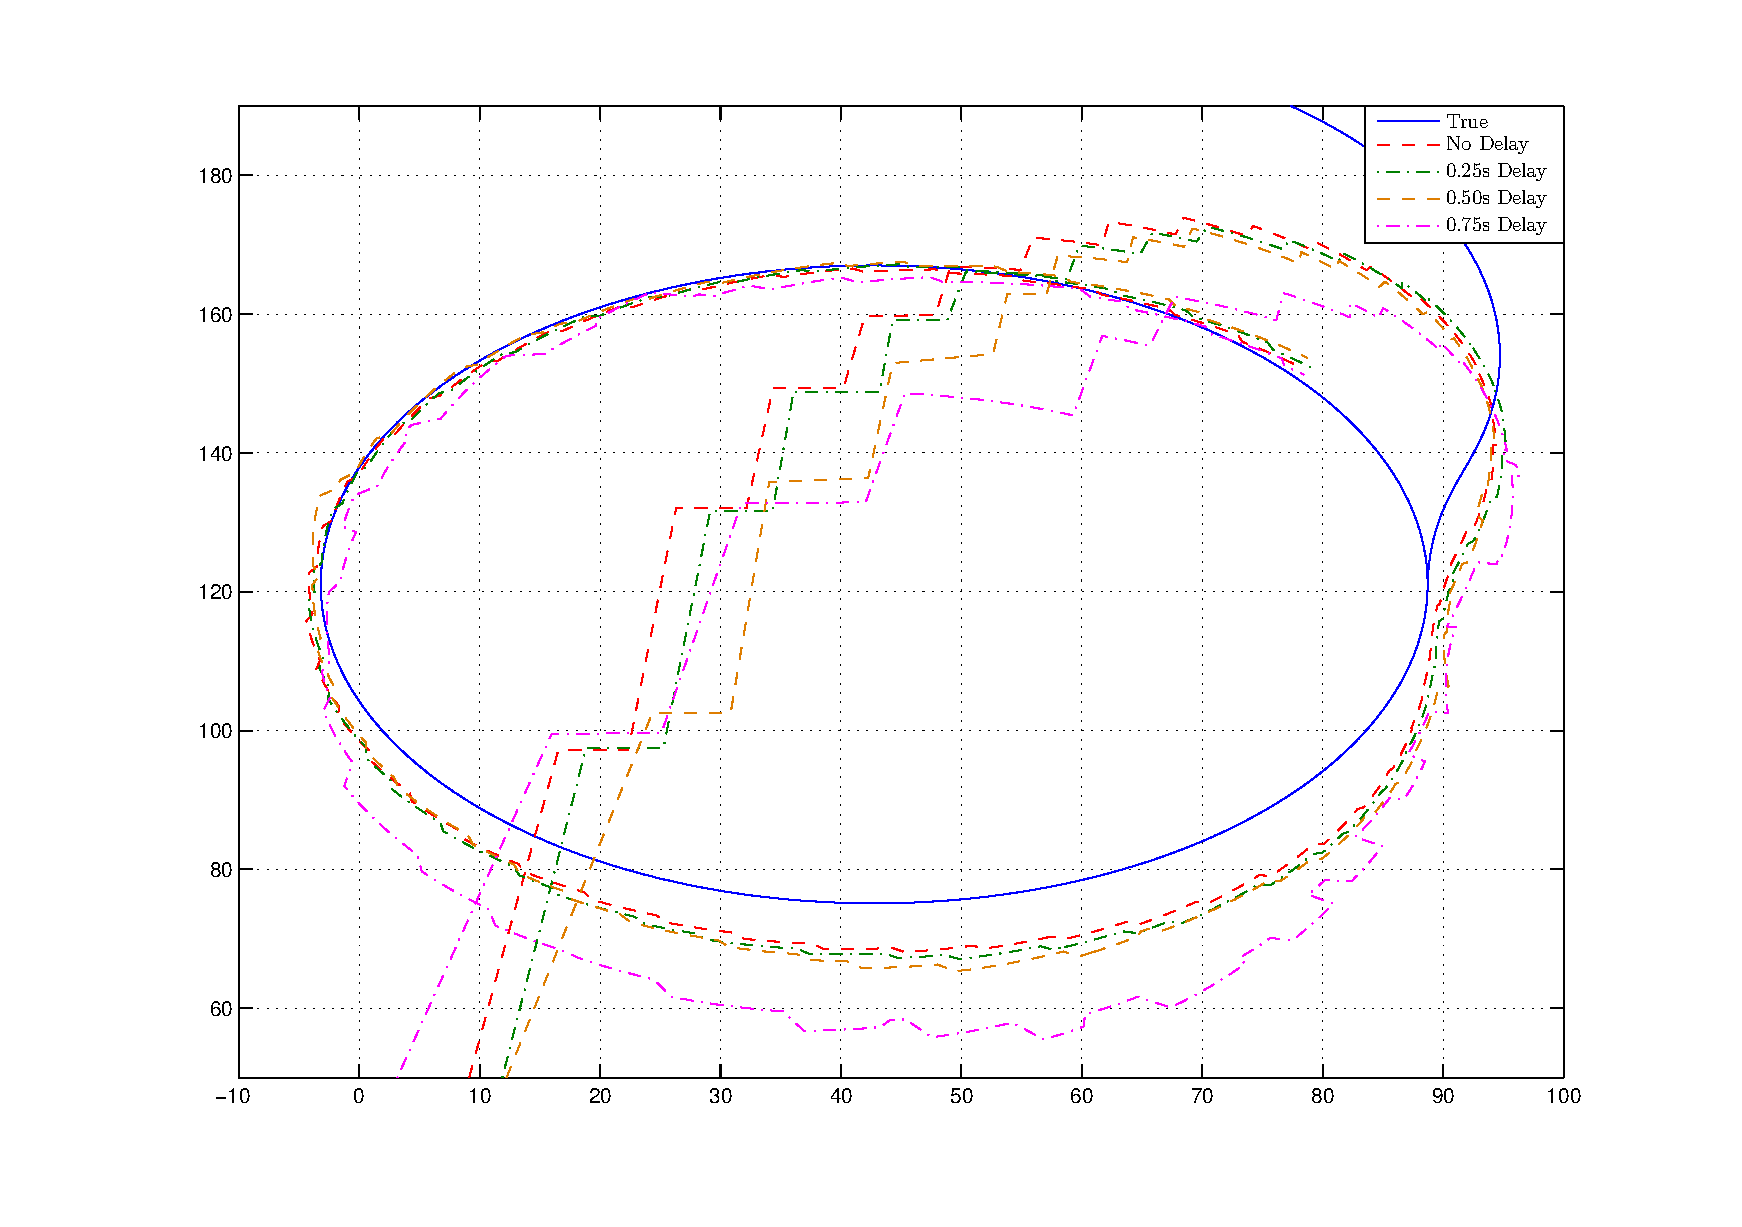
\includegraphics[scale=0.55]{./Results/Delay_Comparison/uav_trajectory.eps}
  \caption[UAV Trajectory Comparison - Different Delays]{UAV Trajectory Comparison - Different Delays. The trajectory of the aircraft is shown in this plot, against the estimated trajectory calculated by a DEKF for no delay, 0.25 s, 0.50 s, and 0.75 s of random delay.}
\end{figure}

\begin{figure}[H]
  \centering
  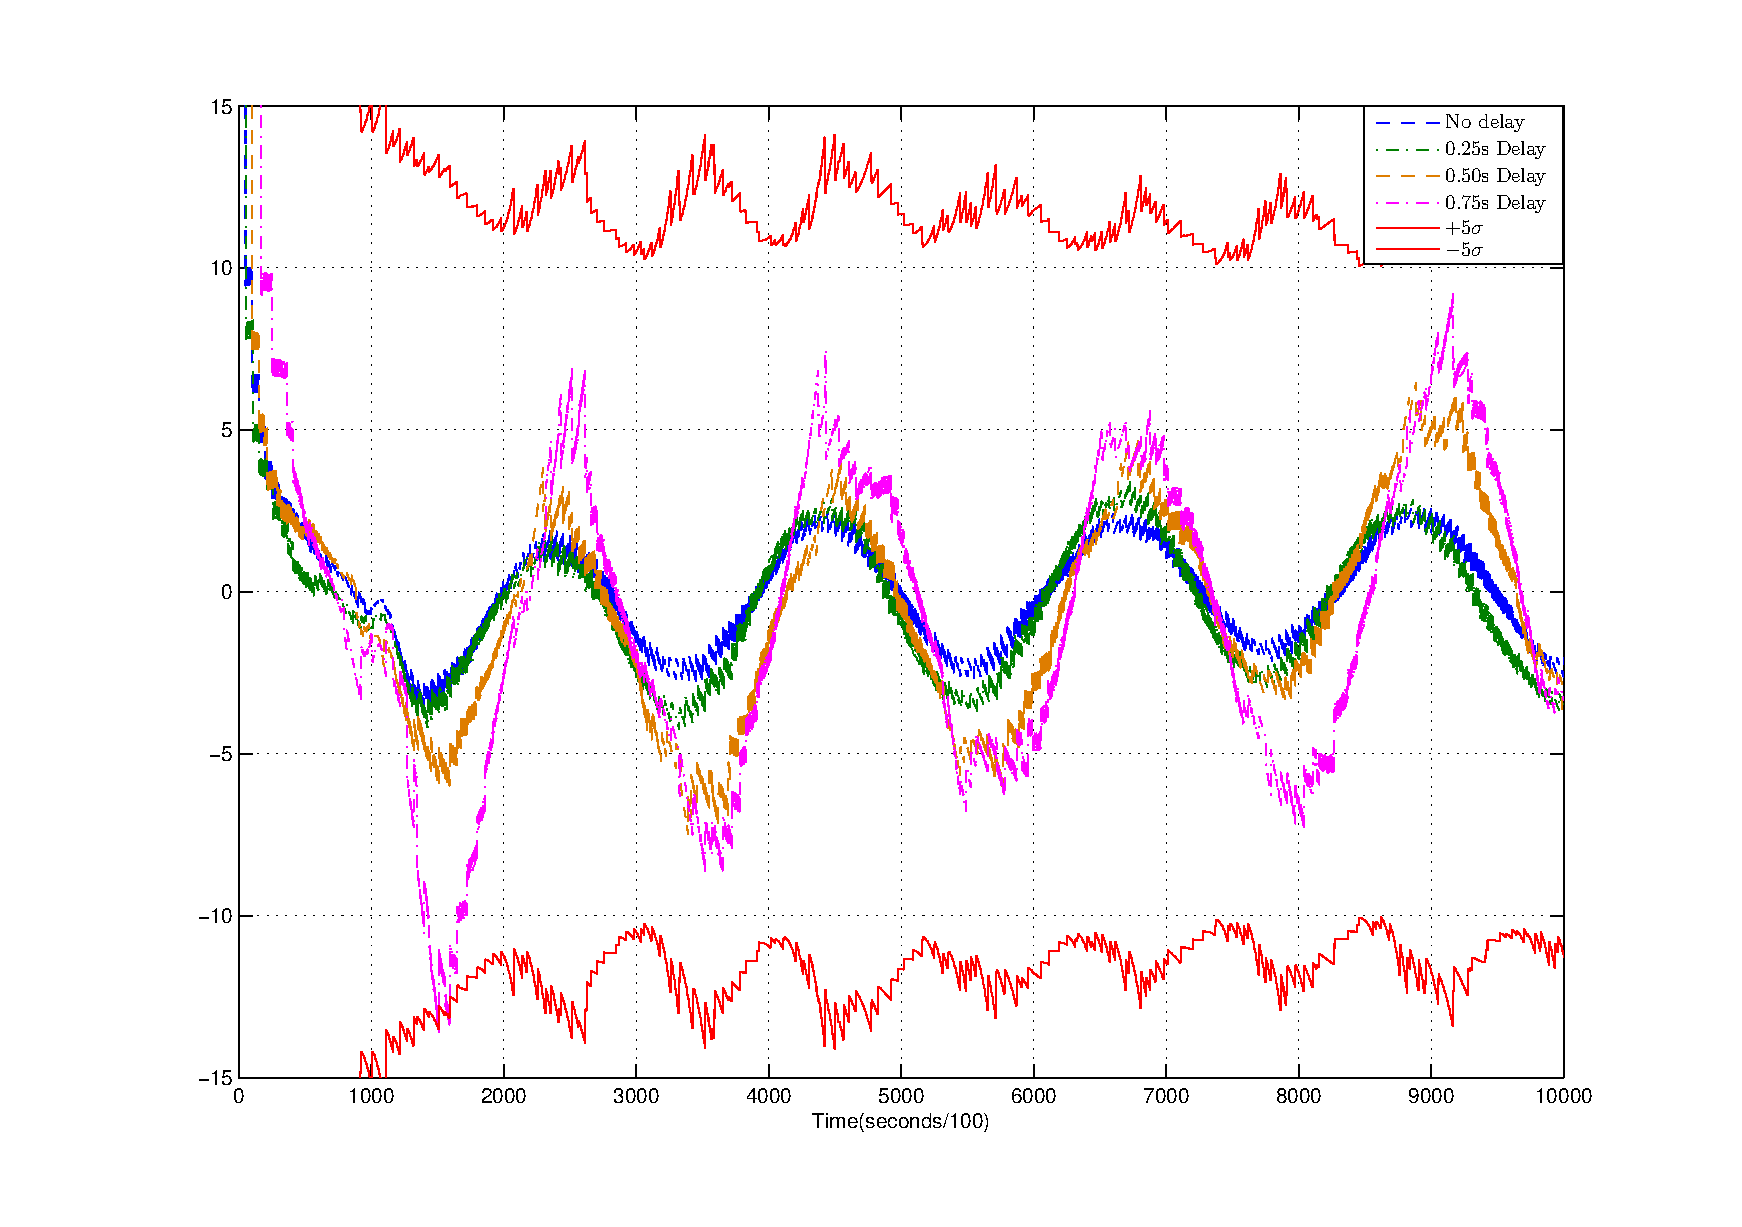
\includegraphics[scale=0.40]{./Results/Delay_Comparison/north_error_comparison.eps}
  \caption[North Position Error Comparison - Different Delays]{North Position Error Comparison - Different Delays. The error in the north position is shown in this plot. The states estimations are compared for no delay, 0.25 s, 0.50 s, and 0.75 s of random delay.}
\end{figure}
\begin{figure}[H]
  \centering
  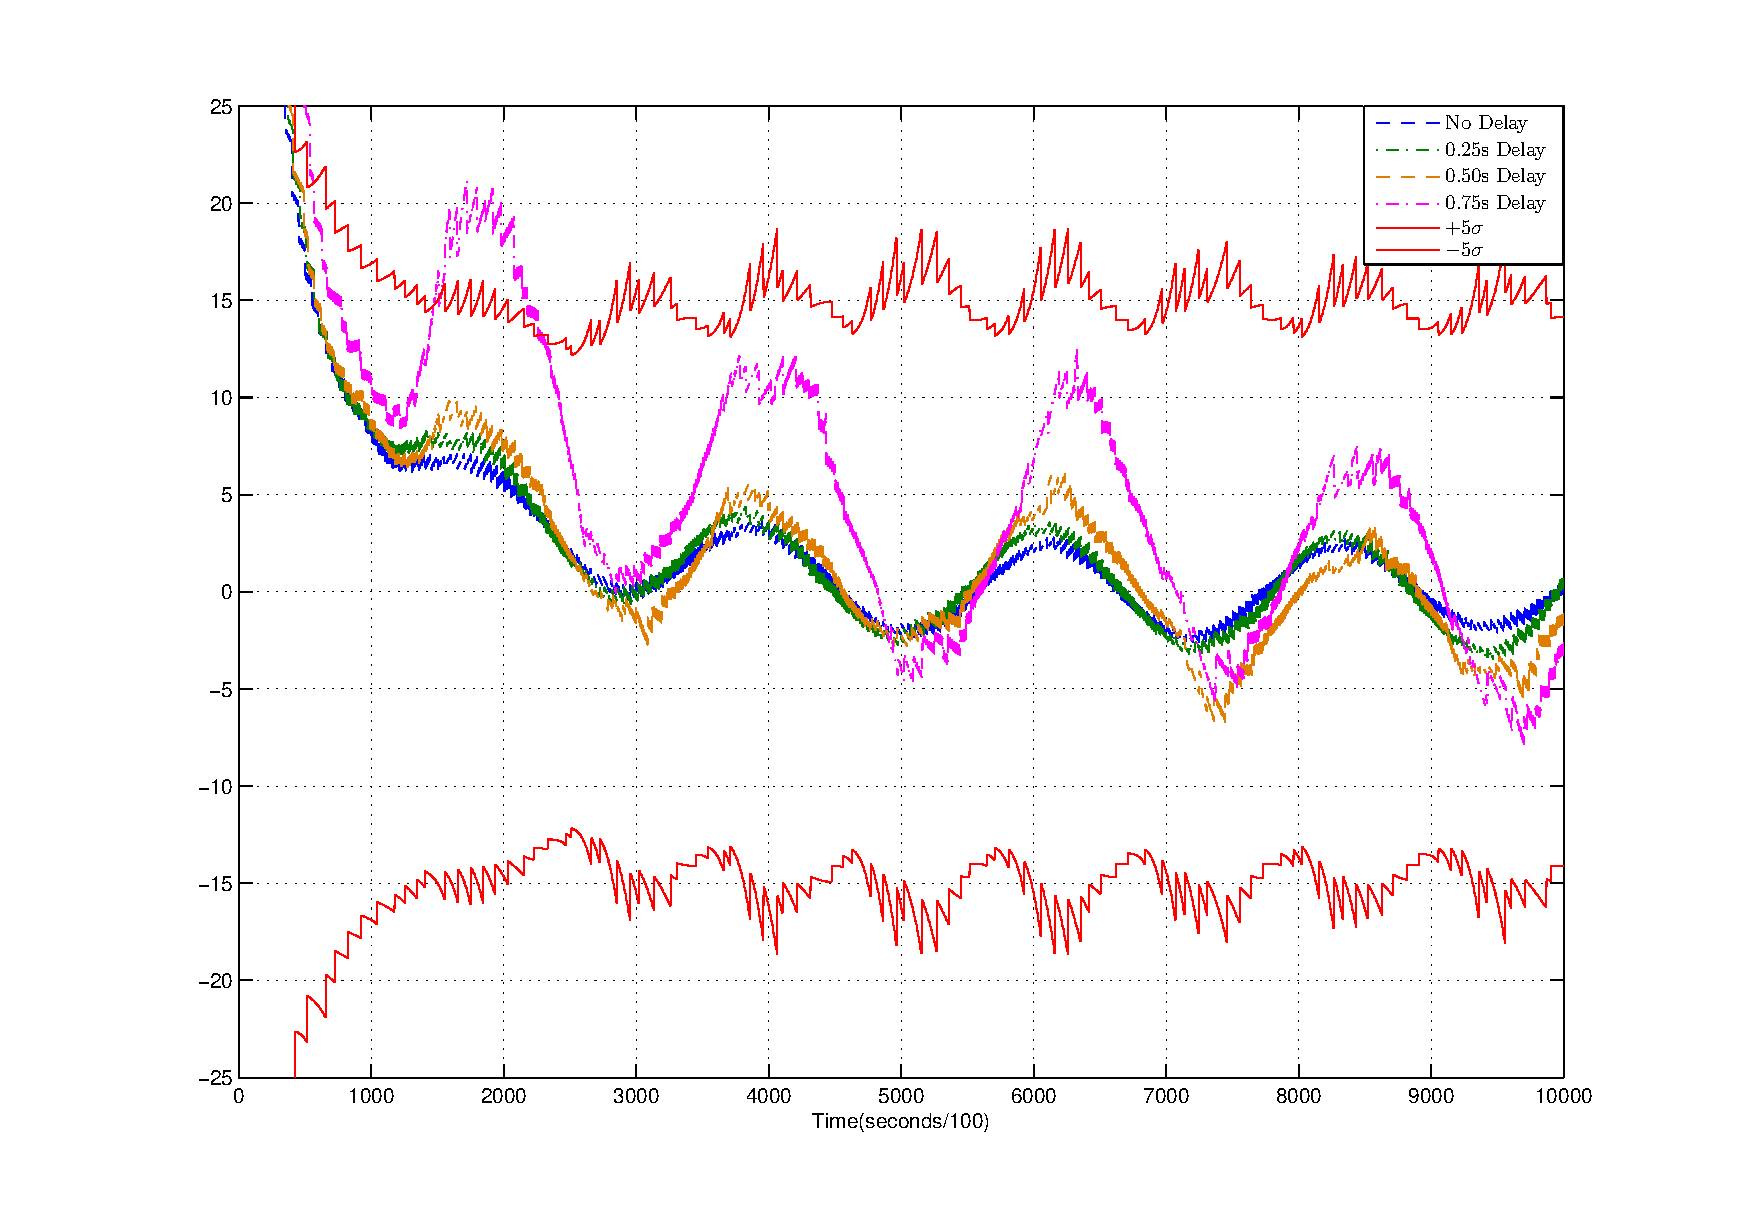
\includegraphics[scale=0.40]{./Results/Delay_Comparison/east_error_comparison.eps}
  \caption[East Position Error Comparison - Different Delays]{East Position Error Comparison - Different Delays. The error in the east position is shown in this plot. The states estimations are compared for no delay, 0.25 s, 0.50 s, and 0.75 s of random delay.}
\end{figure}

\begin{figure}[H]
  \centering
  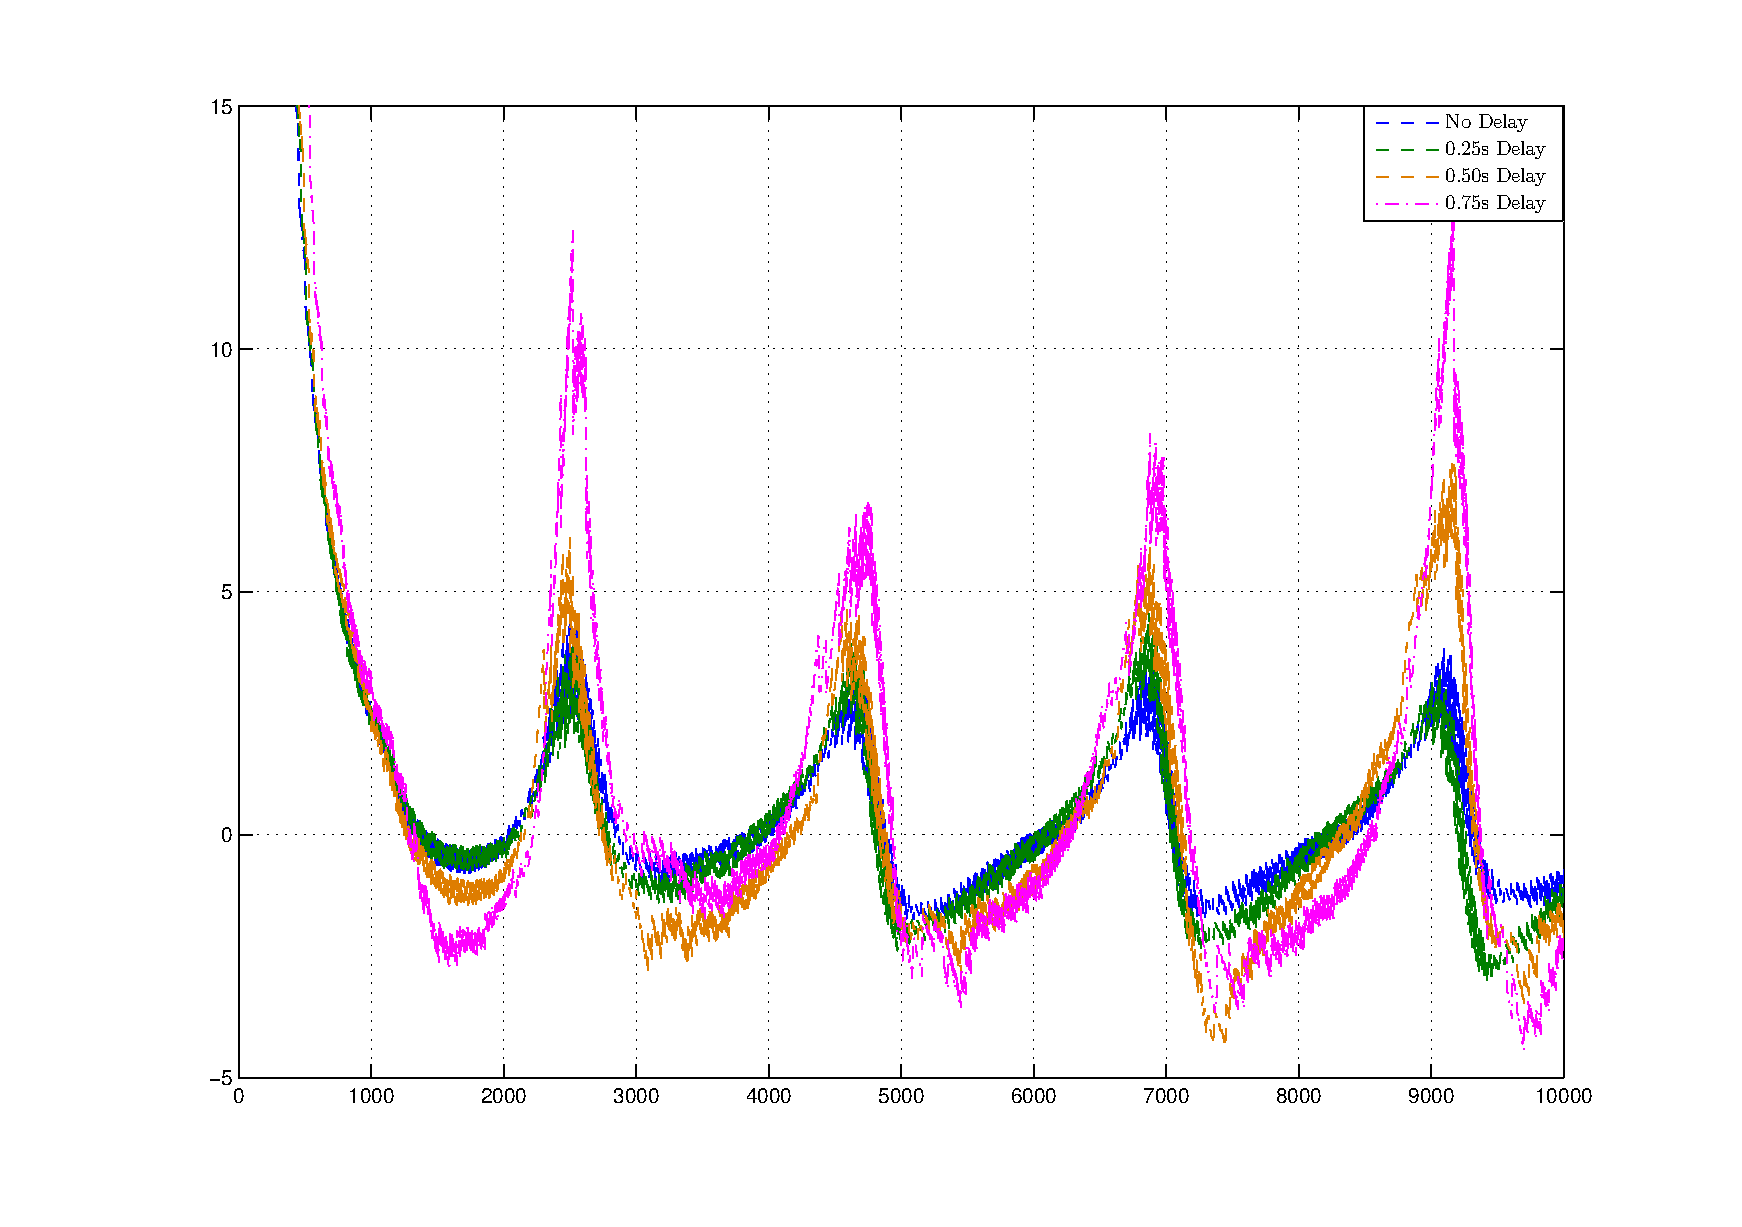
\includegraphics[scale=0.40]{./Results/Delay_Comparison/azimuth_error_comparison.eps}
  \caption[Azimuth Error Comparison - Different Delays]{Azimuth Error Comparison - Different Delays. The error in the azimuth angle calculated by the estimations is shown in this plot. Azimuth for no delay, 0.25 s, 0.50 s, and 0.75 s of random delay, are compared.}
\end{figure}

\begin{figure}[H]
  \centering
  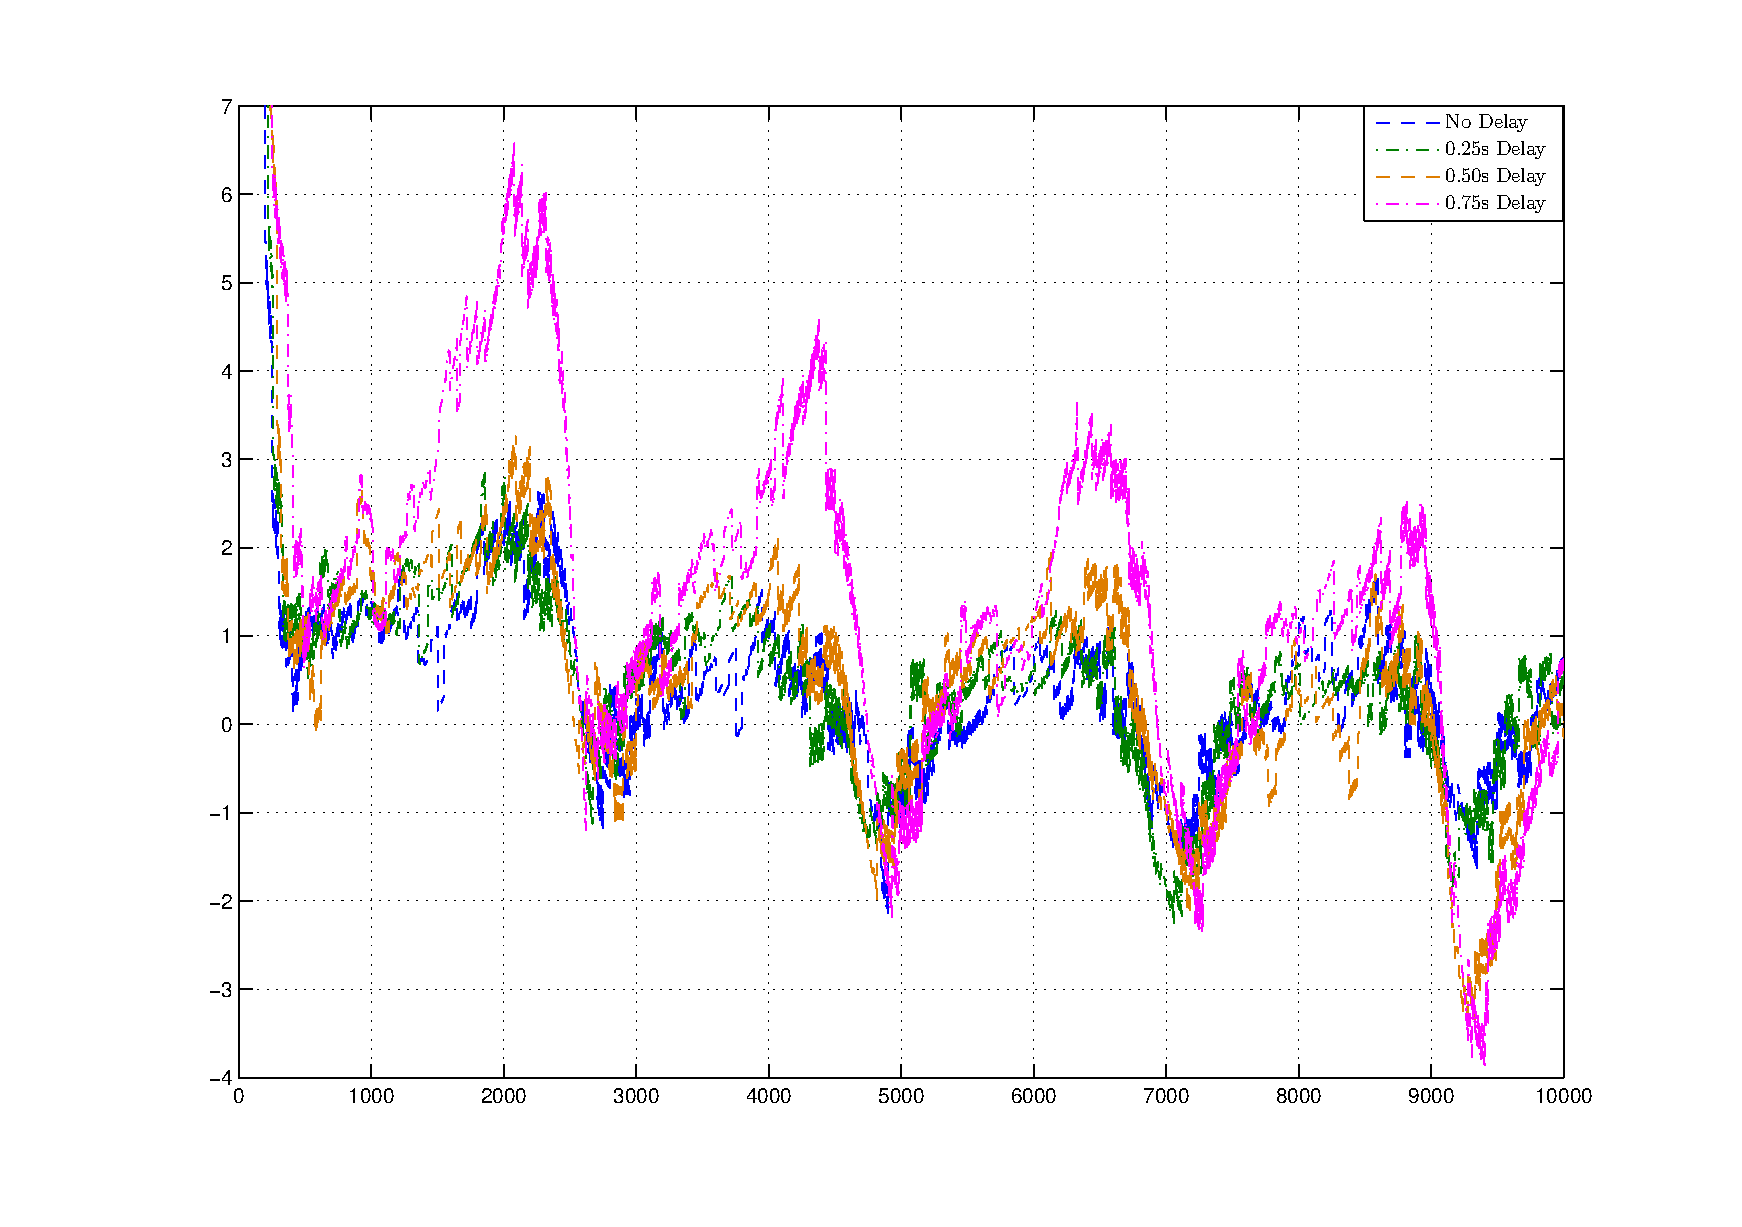
\includegraphics[scale=0.40]{./Results/Delay_Comparison/elevation_error_comparison.eps}
  \caption[Elevation Error Comparison - Different Delays]{Elevation Error Comparison - Different Delays. The error in the elevation angle calculated by the estimations is shown in this plot. Elevation for no delay, 0.25 s, 0.50 s, and 0.75 s of random delay, are compared.}
\end{figure}

%
%\subsection{Case 3 - GPS Sensor With Fixed Delay of 0.25 sec} \hspace{0pt} \\
%In this case, all the measurements are delayed 0.25 s. The delayed extended Kalman filter is used from now on.
%
%\begin{figure}[h!]
%  \centering
%  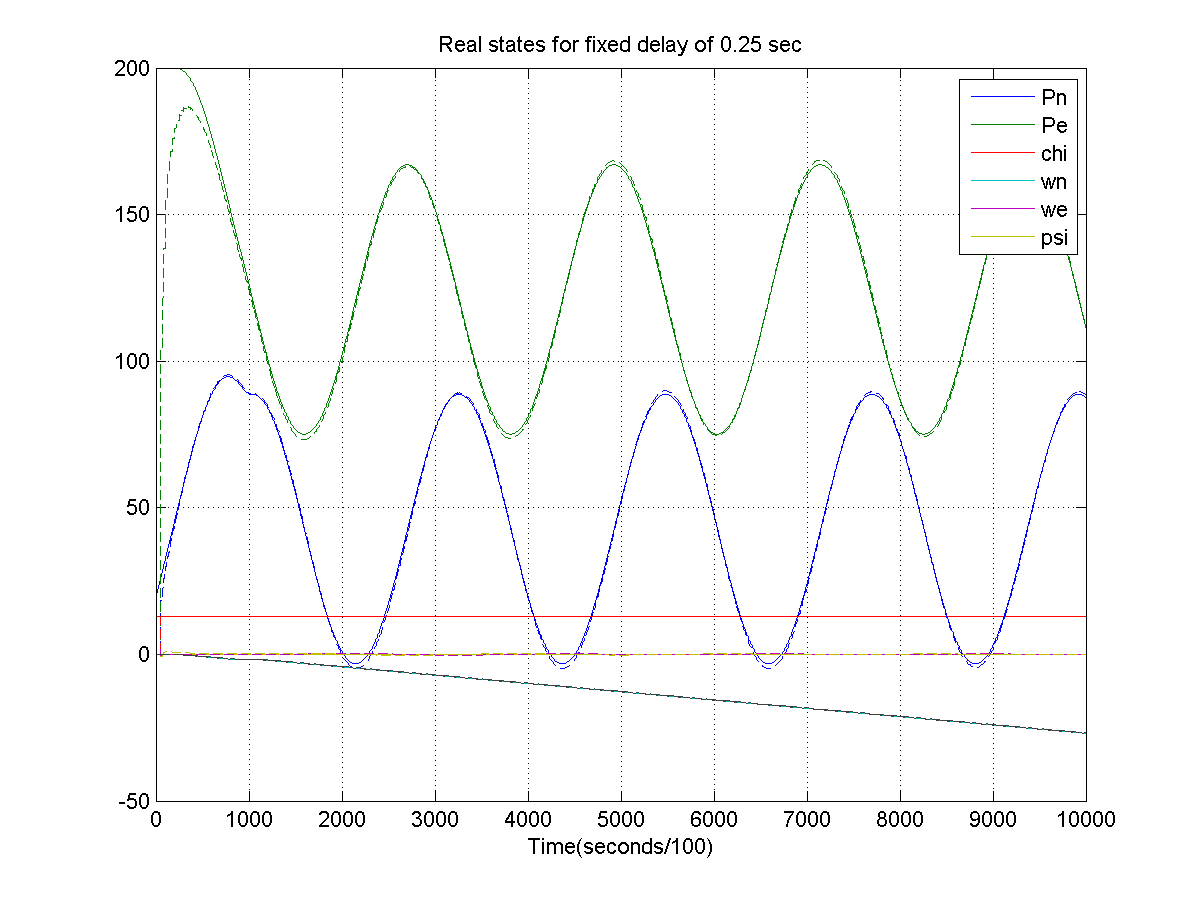
\includegraphics[scale=0.6]{./GPS/fixed_delay_0.25/fig4}
%  \caption{Real States vs Estimated States - Case 3}
%\end{figure}
%\pagebreak
%\begin{figure}[h!]
%  \centering
%  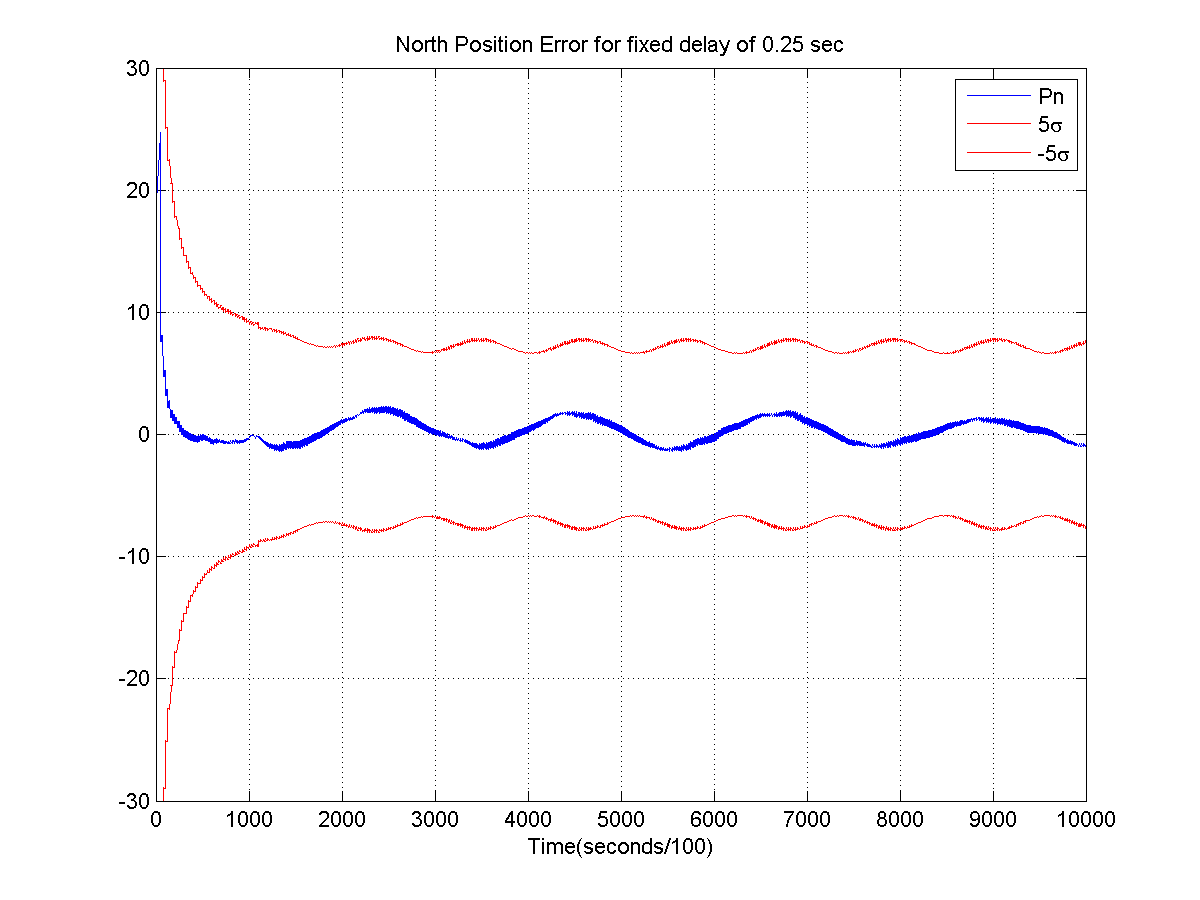
\includegraphics[scale=0.6]{./GPS/fixed_delay_0.25/fig5}
%  \caption{North Position Error - Case 3}
%\end{figure}
%\begin{figure}[h!]
%  \centering
%  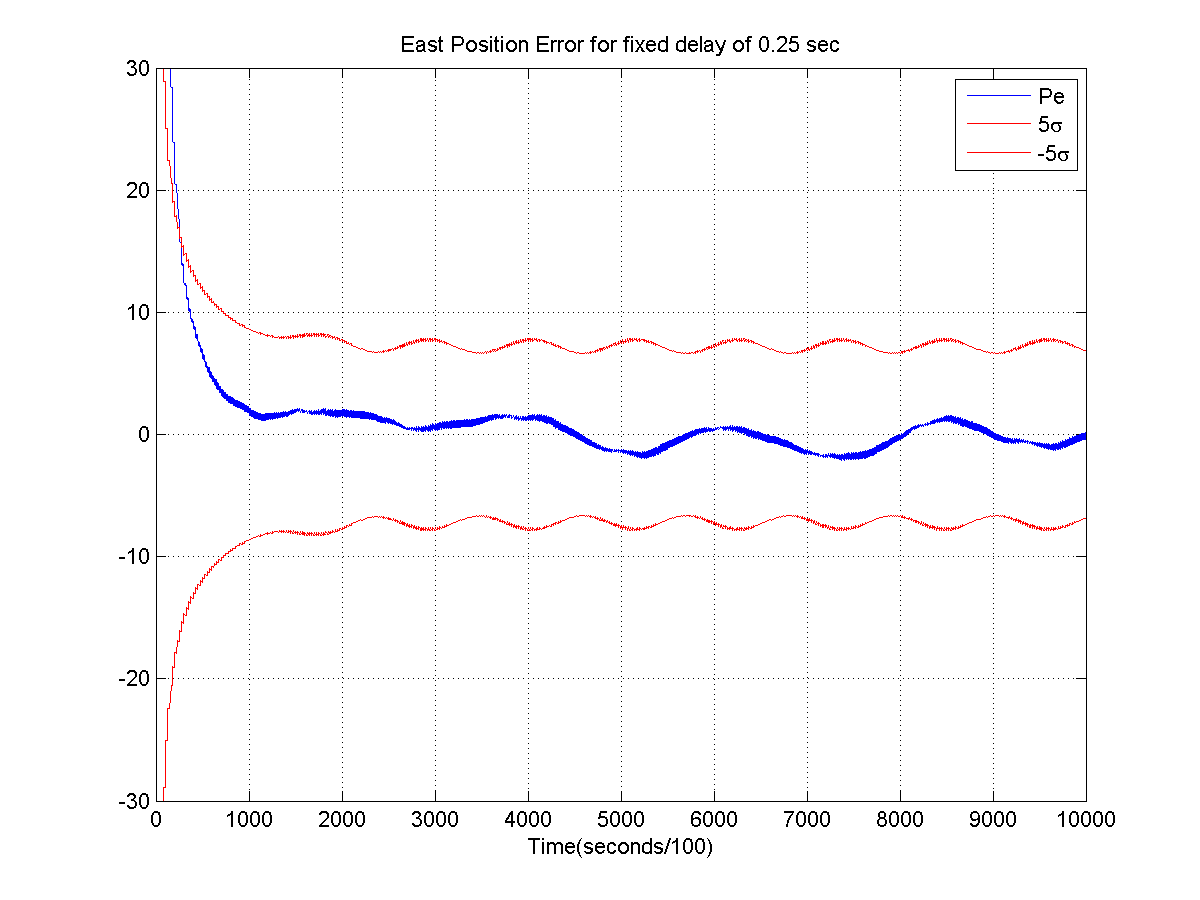
\includegraphics[scale=0.6]{./GPS/fixed_delay_0.25/fig6}
%  \caption{East Position Error - Case 3}
%  \label{fig:theFig}
%\end{figure}
%\begin{figure}[h!]
%  \centering
%  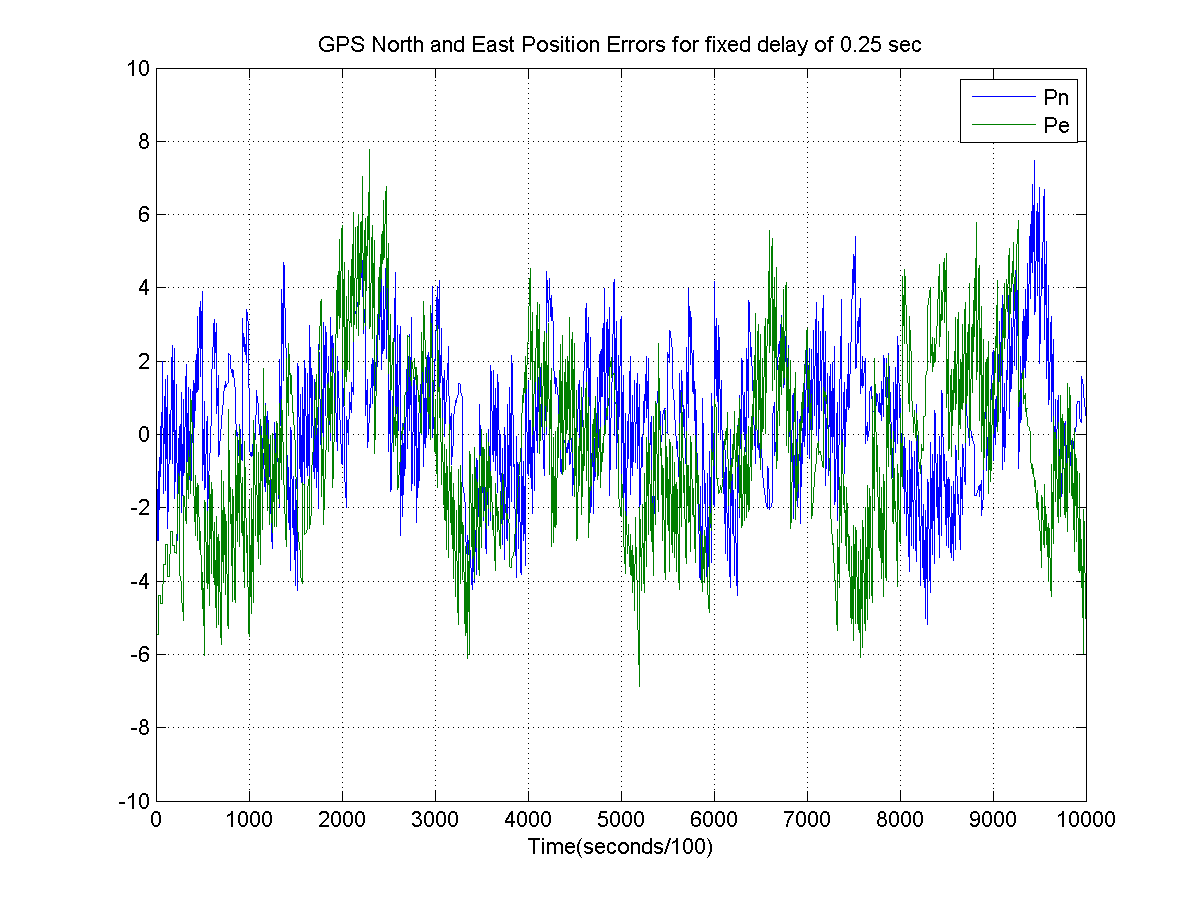
\includegraphics[scale=0.6]{./GPS/fixed_delay_0.25/fig7}
%  \caption{GPS Position Error - Case 3}
%  \label{fig:theFig}
%\end{figure}
%
%\begin{figure}[h!]
%  \centering
%  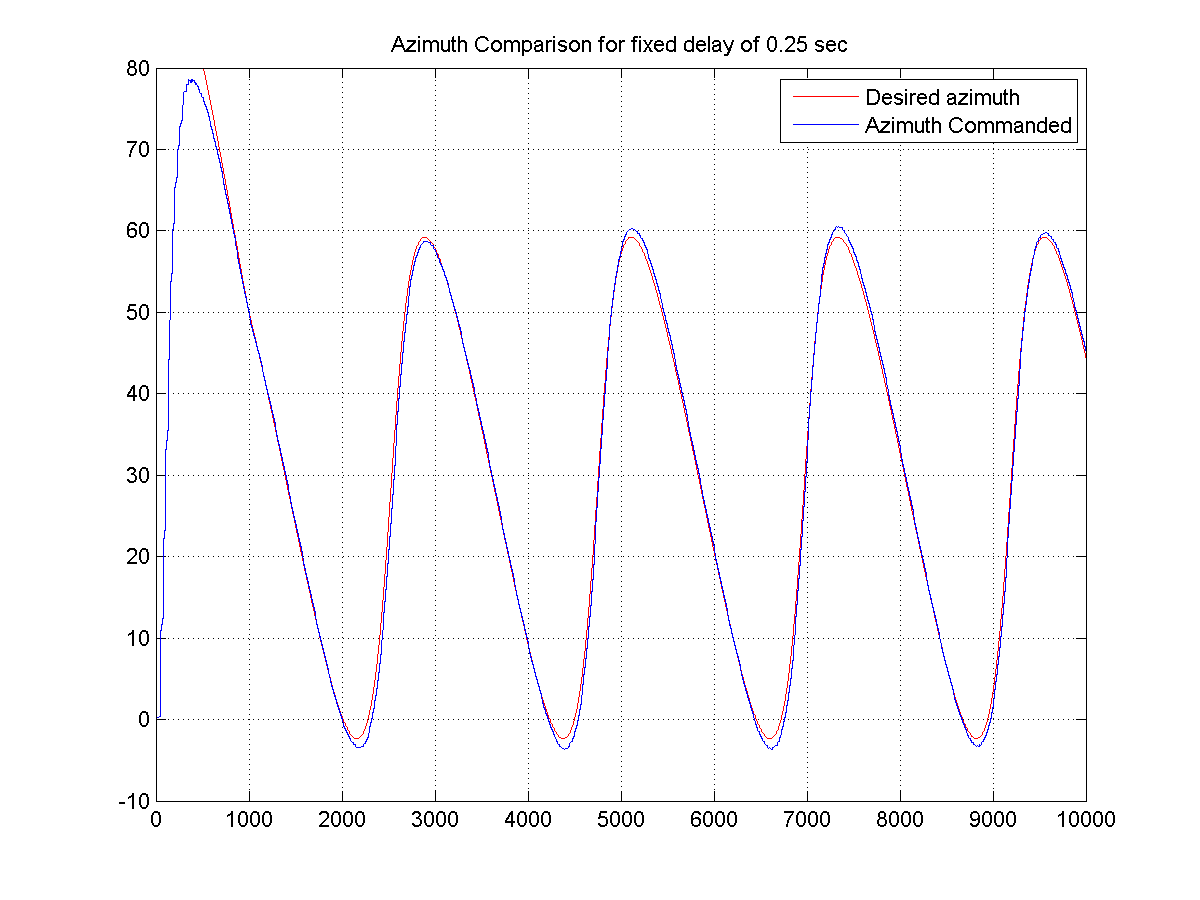
\includegraphics[scale=0.6]{./GPS/fixed_delay_0.25/fig8}
%  \caption{Desired Azimuth vs Estimated Azimuth - Case 3}
%  \label{fig:theFig}
%\end{figure}
%\begin{figure}[h!]
%  \centering
%  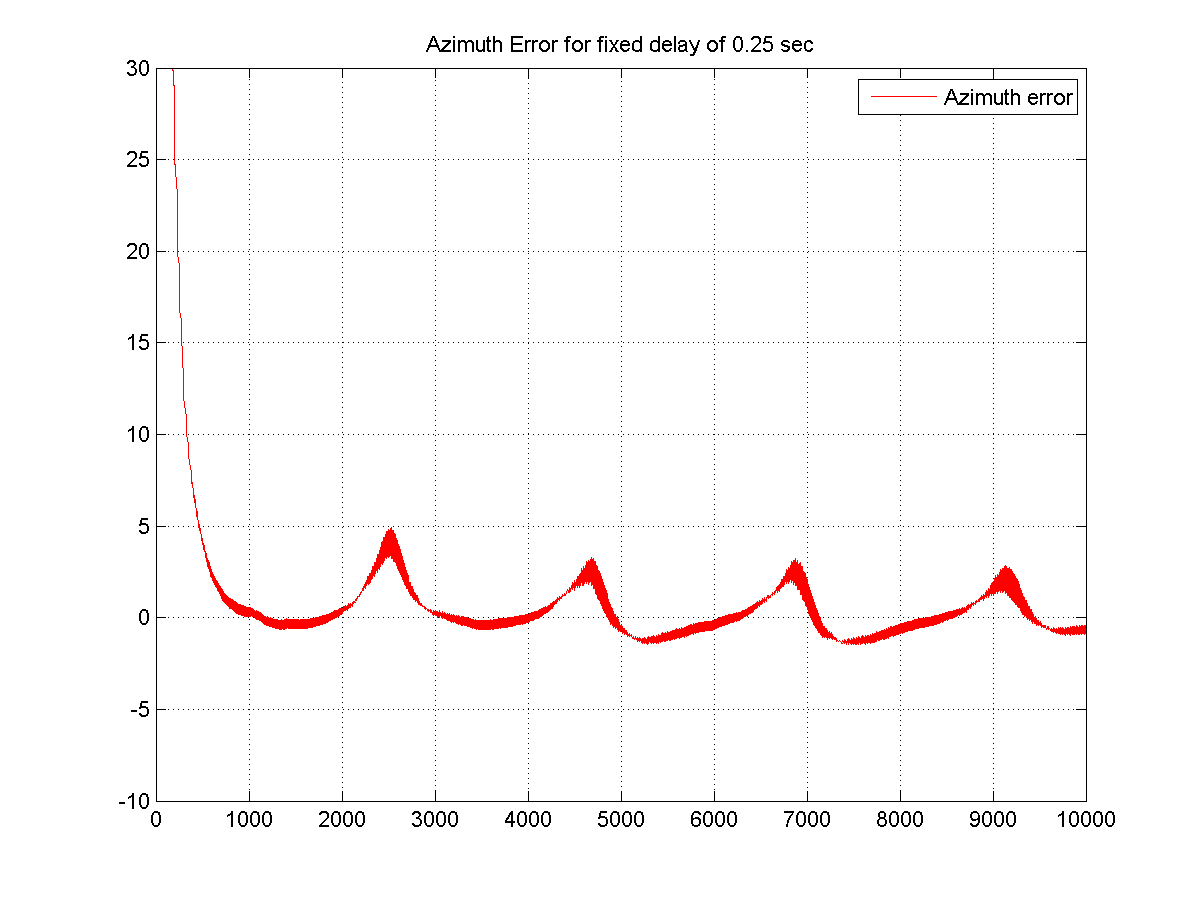
\includegraphics[scale=0.6]{./GPS/fixed_delay_0.25/fig9}
%  \caption{Azimuth Error - Case 3}
%  \label{fig:theFig}
%\end{figure}
%\begin{figure}[h!]
%  \centering
%  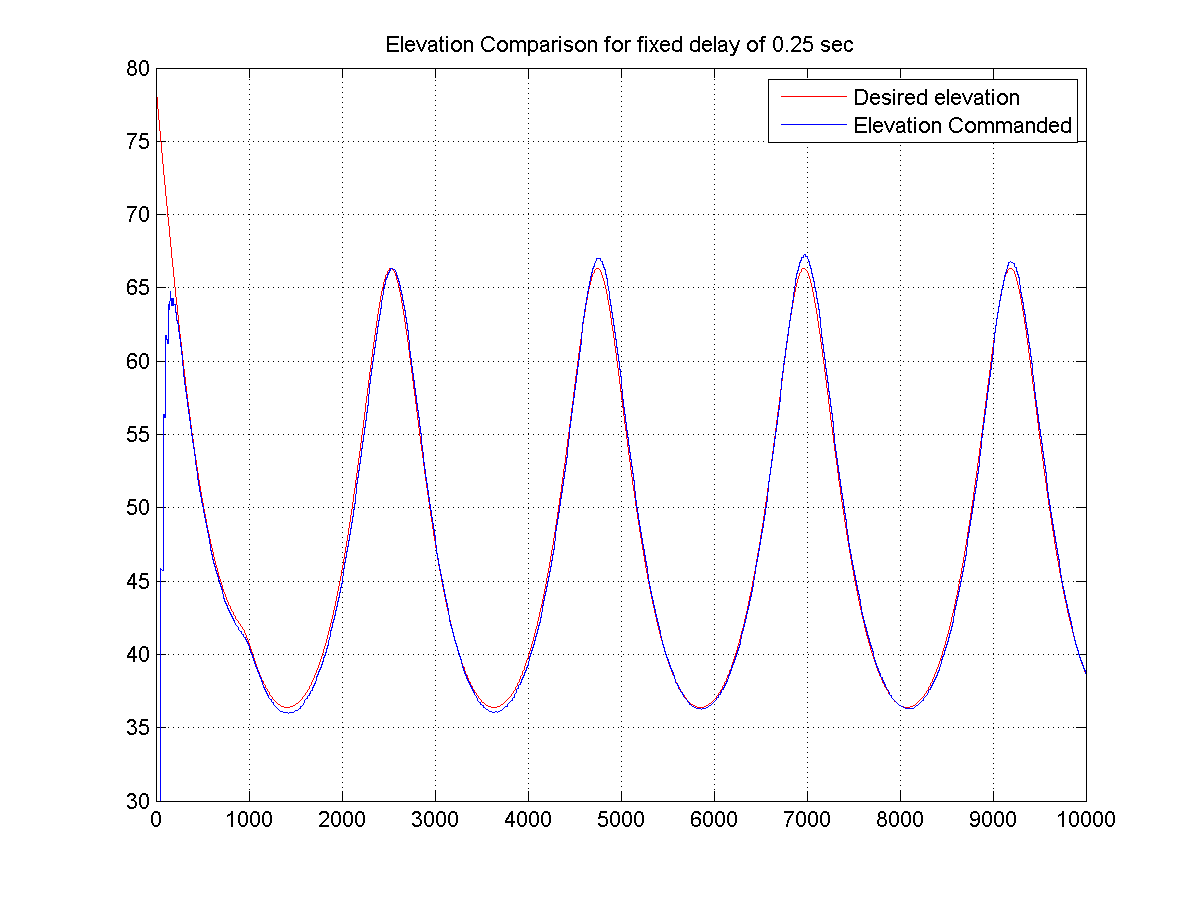
\includegraphics[scale=0.6]{./GPS/fixed_delay_0.25/fig10}
%  \caption{Desired Elevation vs Estimated Elevation - Case 3}
%  \label{fig:theFig}
%\end{figure}
%\begin{figure}[h!]
%  \centering
%  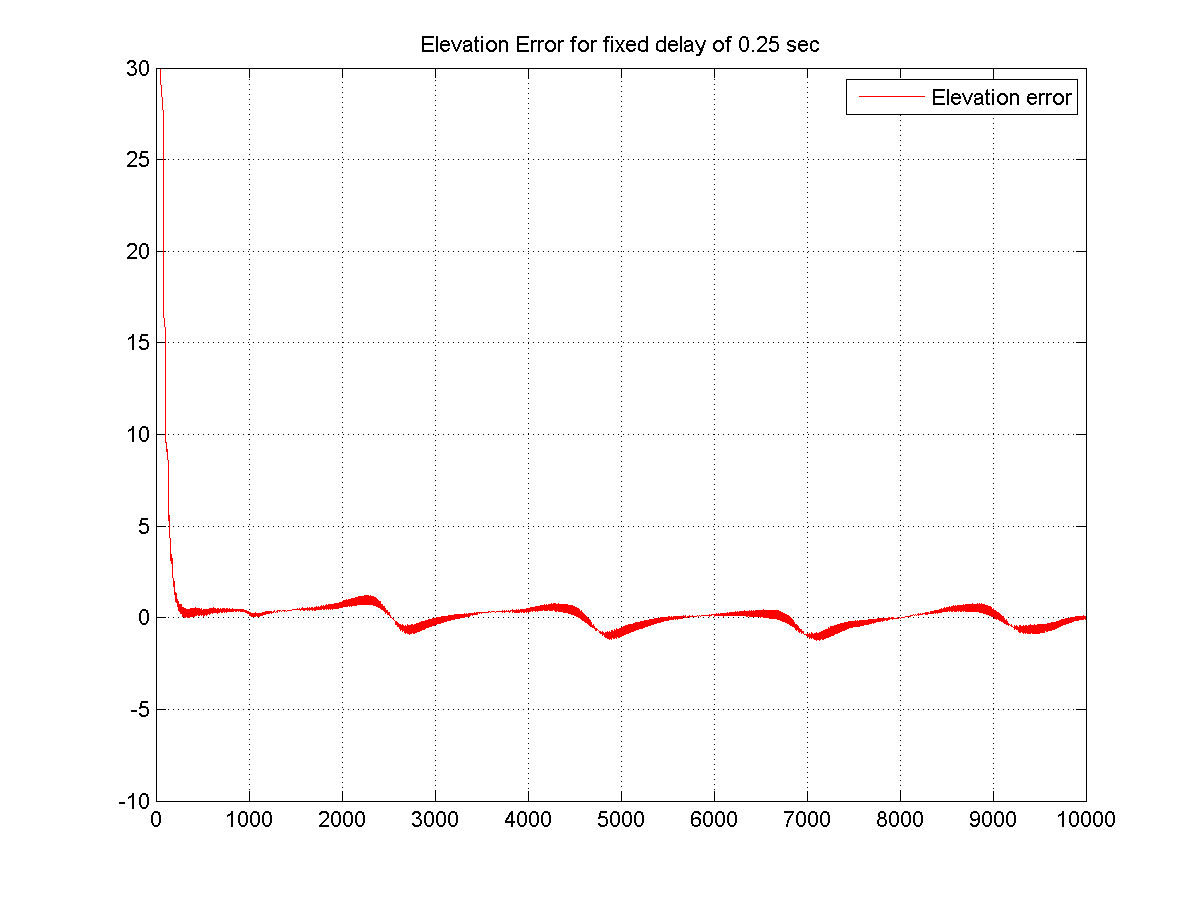
\includegraphics[scale=0.6]{./GPS/fixed_delay_0.25/fig11}
%  \caption{Elevation Error - Case 3}
%  \label{fig:theFig}
%\end{figure}
%\begin{figure}[h!]
%  \centering
%  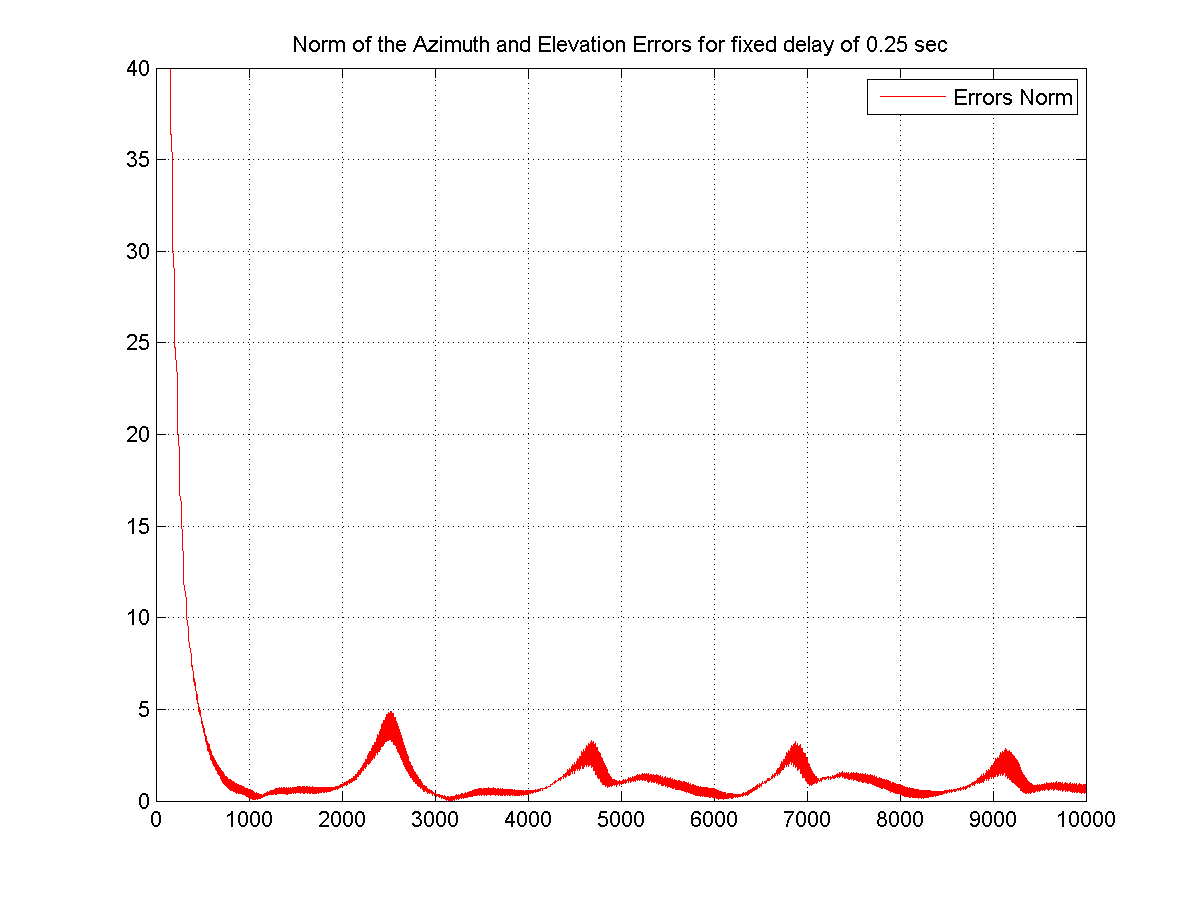
\includegraphics[scale=0.6]{./GPS/fixed_delay_0.25/fig12}
%  \caption{Normalized Azimuth and Elevation Errors - Case 3}
%  \label{fig:theFig}
%\end{figure}
%
%\subsection{Case 4 - GPS Sensor With Fixed Delay of 0.25 sec Disregarding Delay} \hspace{0pt} \\
%In this case, all the measurements are delayed 0.25 s. The difference is that a regular Extended Kalman filter is used, that means that the delays are not taking into account in the filter. This is done for comparison purposes.
%
%\begin{figure}[h!]
%  \centering
%  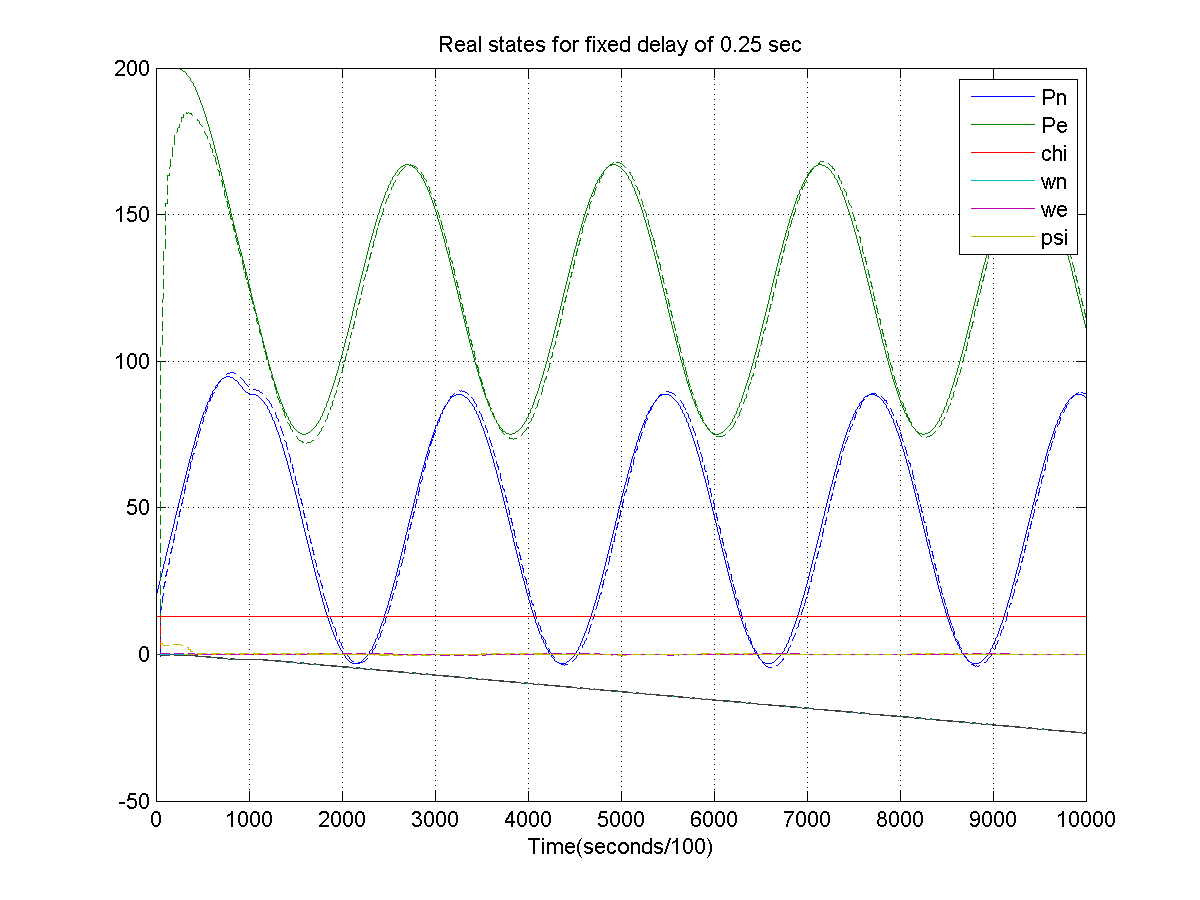
\includegraphics[scale=0.6]{./GPS_EKF/fixed_delay_0.25/fig4}
%  \caption{Real States vs Estimated States - Case 4}
%\end{figure}
%\pagebreak
%\begin{figure}[h!]
%  \centering
%  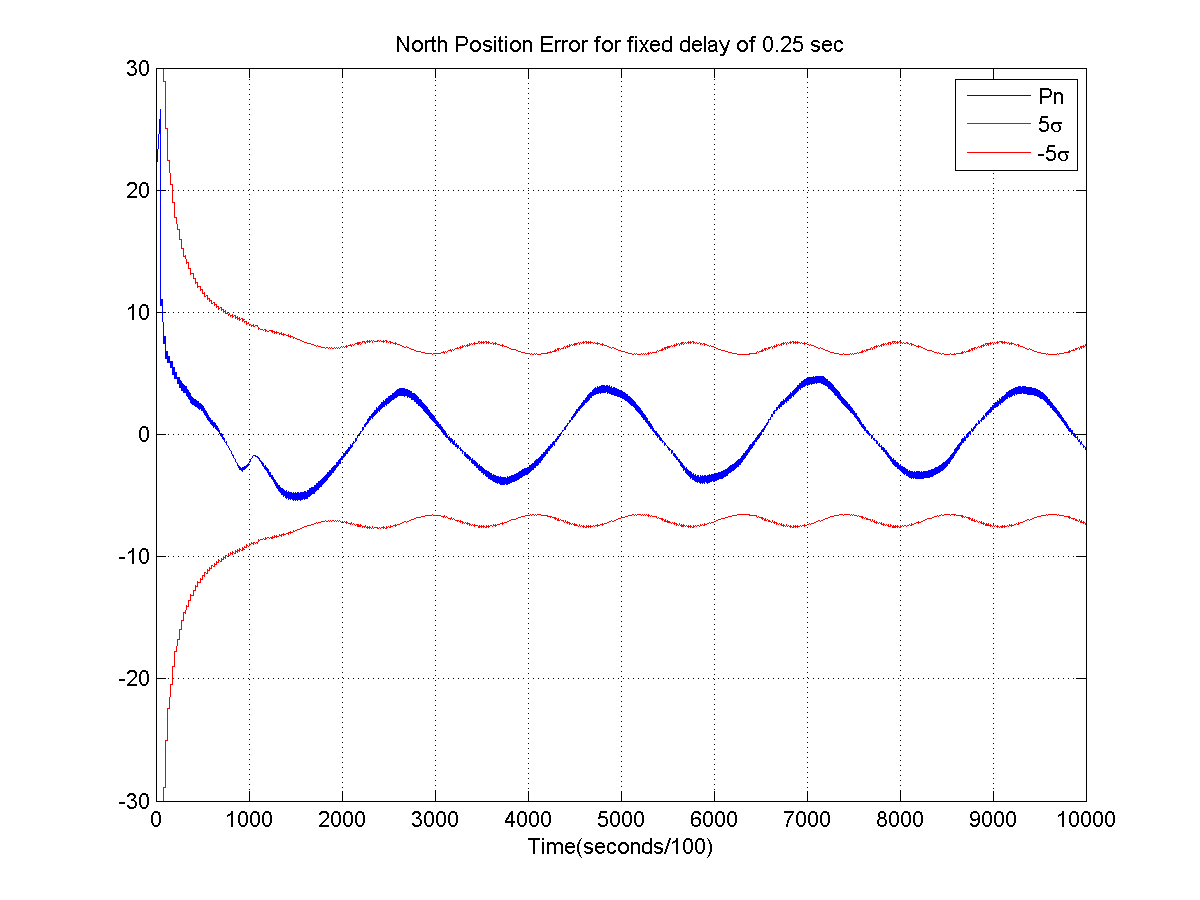
\includegraphics[scale=0.6]{./GPS_EKF/fixed_delay_0.25/fig5}
%  \caption{North Position Error - Case 4}
%\end{figure}
%\begin{figure}[h!]
%  \centering
%  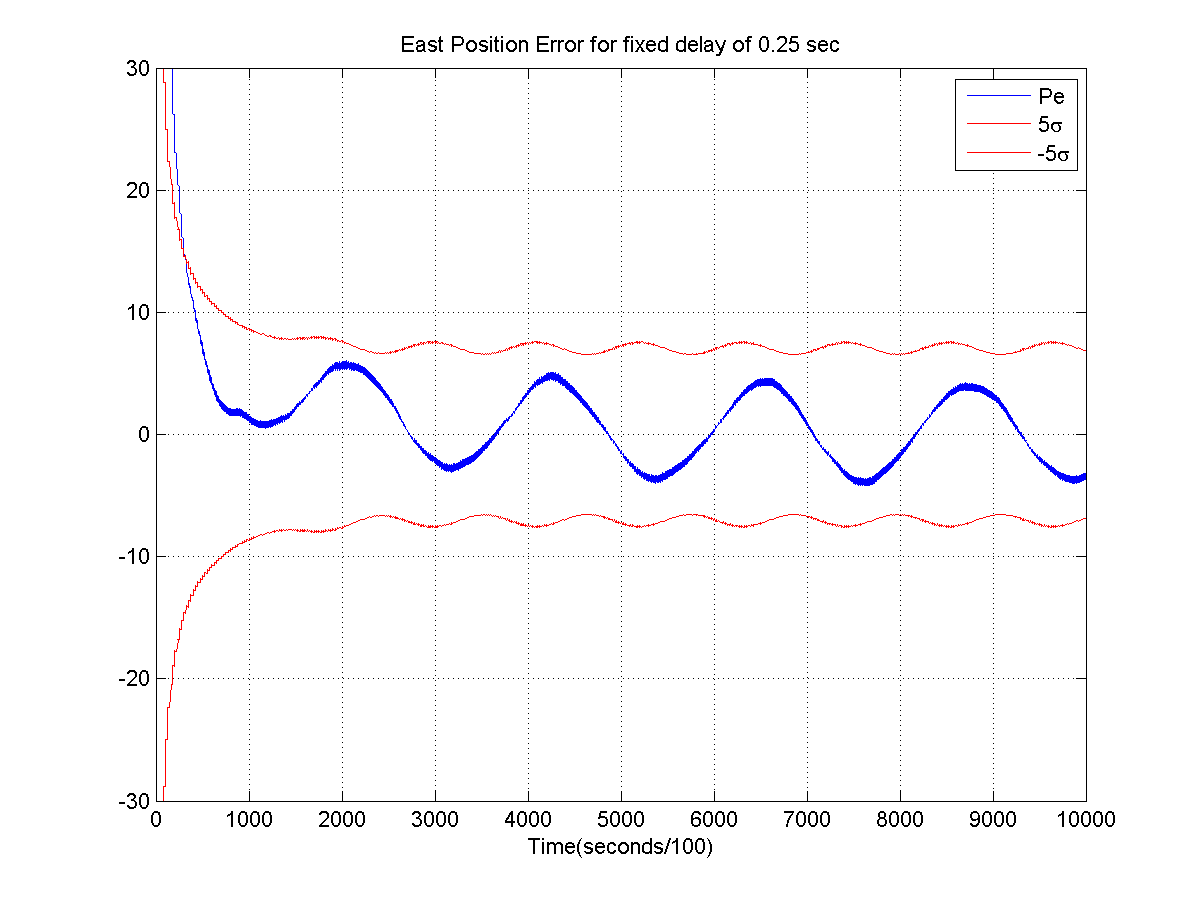
\includegraphics[scale=0.6]{./GPS_EKF/fixed_delay_0.25/fig6}
%  \caption{East Position Error - Case 4}
%  \label{fig:theFig}
%\end{figure}
%\begin{figure}[h!]
%  \centering
%  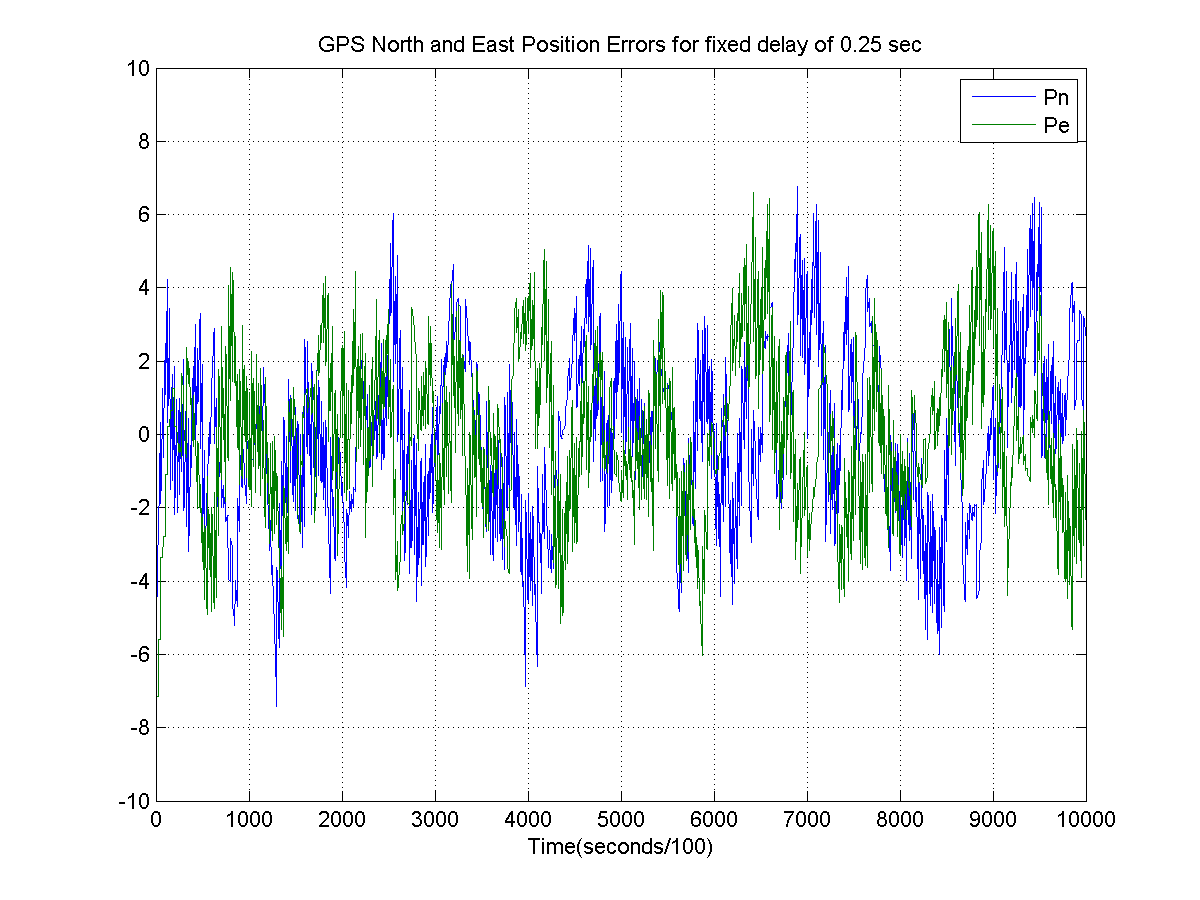
\includegraphics[scale=0.6]{./GPS_EKF/fixed_delay_0.25/fig7}
%  \caption{GPS Position Error - Case 4}
%  \label{fig:theFig}
%\end{figure}
%
%\begin{figure}[h!]
%  \centering
%  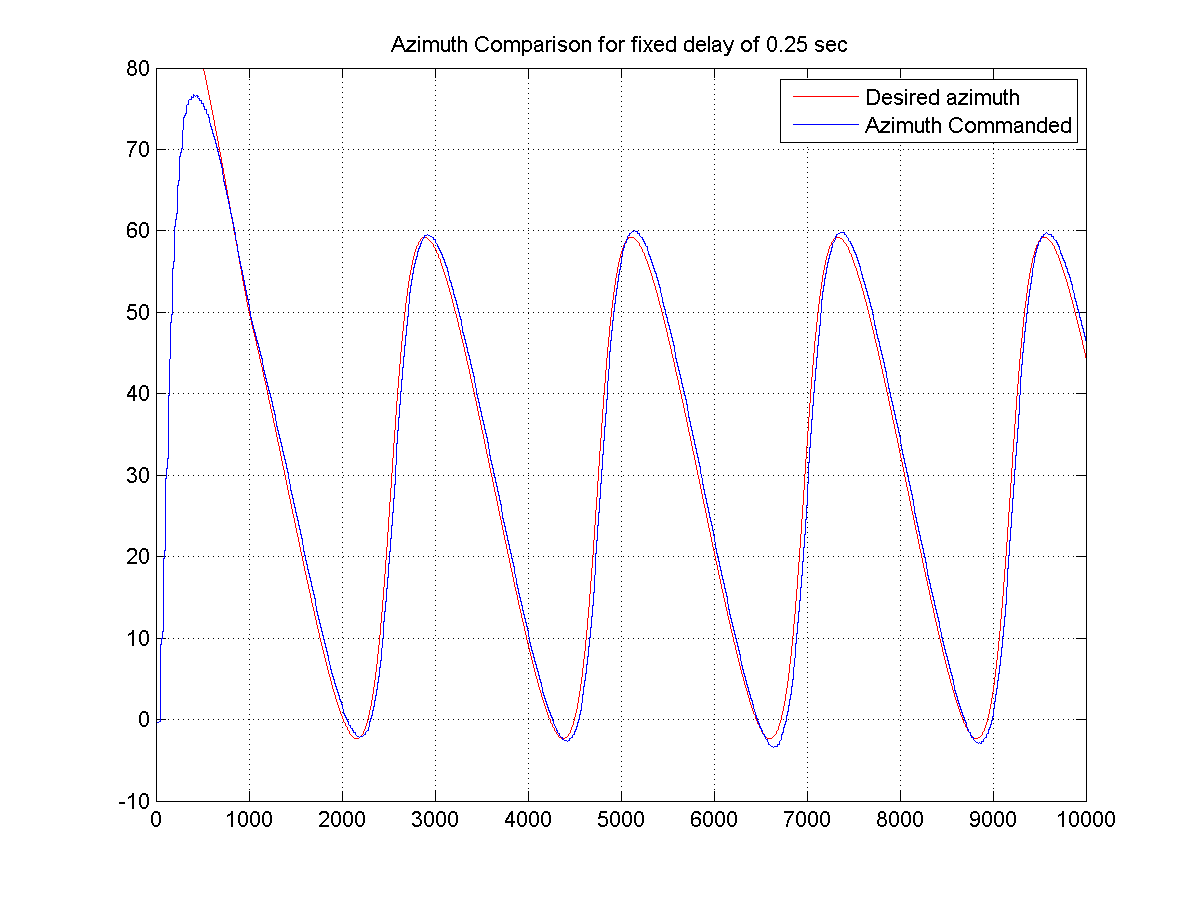
\includegraphics[scale=0.6]{./GPS_EKF/fixed_delay_0.25/fig8}
%  \caption{Desired Azimuth vs Estimated Azimuth - Case 4}
%  \label{fig:theFig}
%\end{figure}
%\begin{figure}[h!]
%  \centering
%  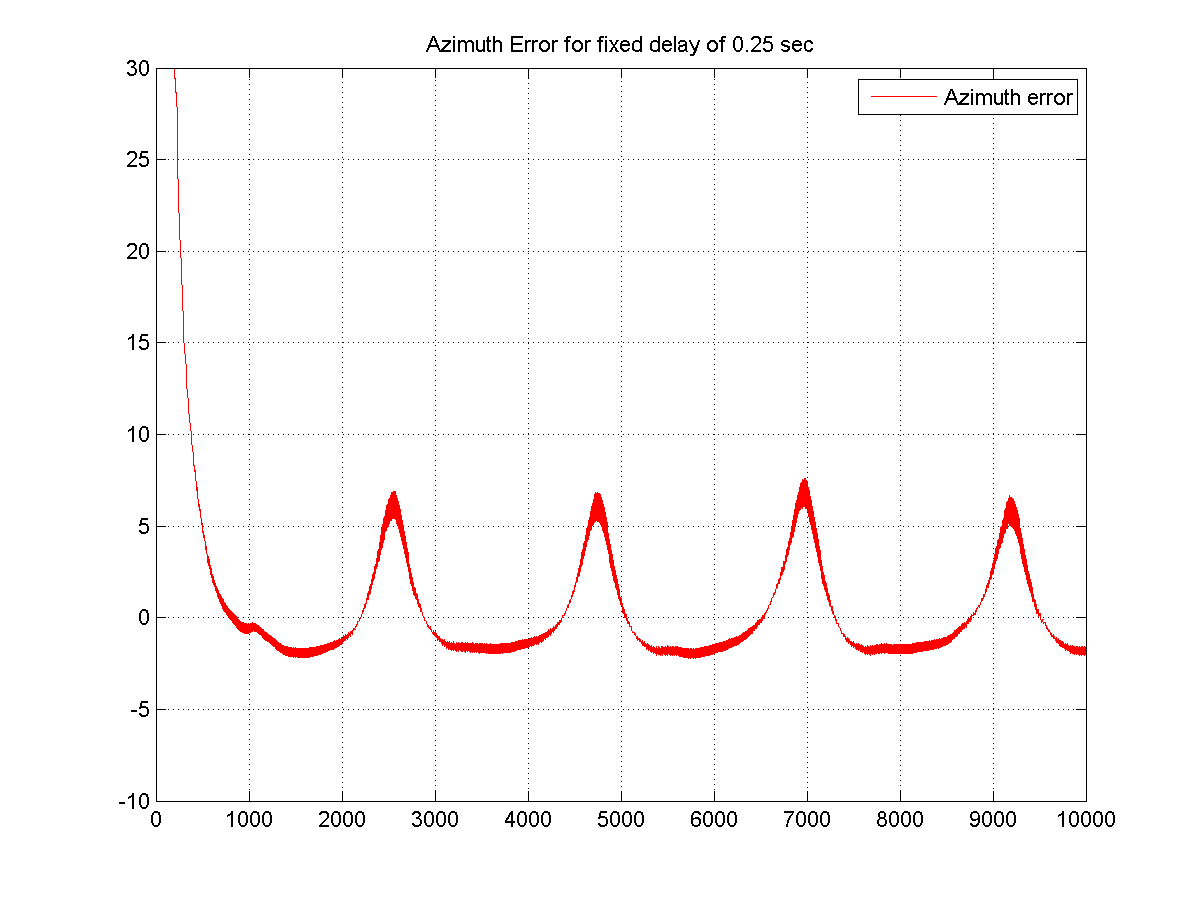
\includegraphics[scale=0.6]{./GPS_EKF/fixed_delay_0.25/fig9}
%  \caption{Azimuth Error - Case 4}
%  \label{fig:theFig}
%\end{figure}
%\begin{figure}[h!]
%  \centering
%  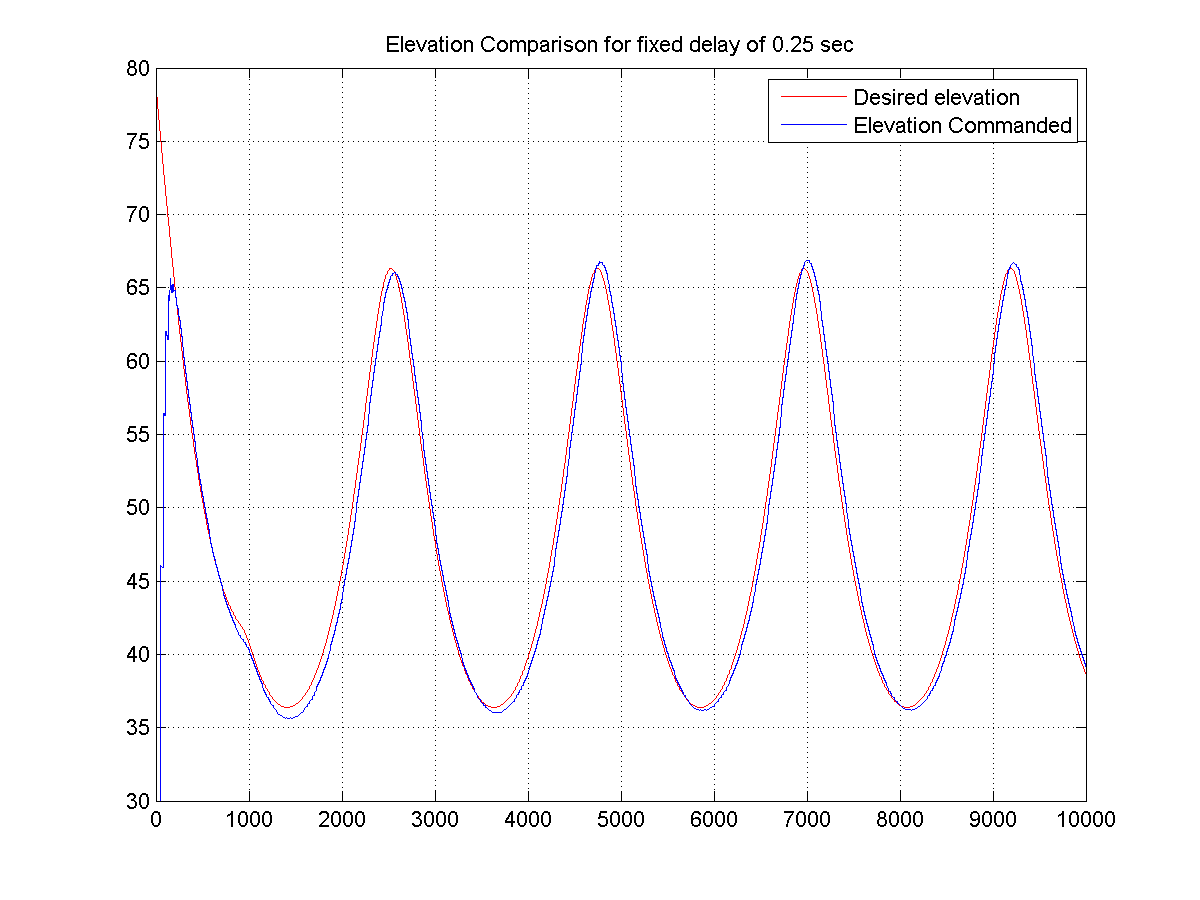
\includegraphics[scale=0.6]{./GPS_EKF/fixed_delay_0.25/fig10}
%  \caption{Desired Elevation vs Estimated Elevation - Case 4}
%  \label{fig:theFig}
%\end{figure}
%\begin{figure}[h!]
%  \centering
%  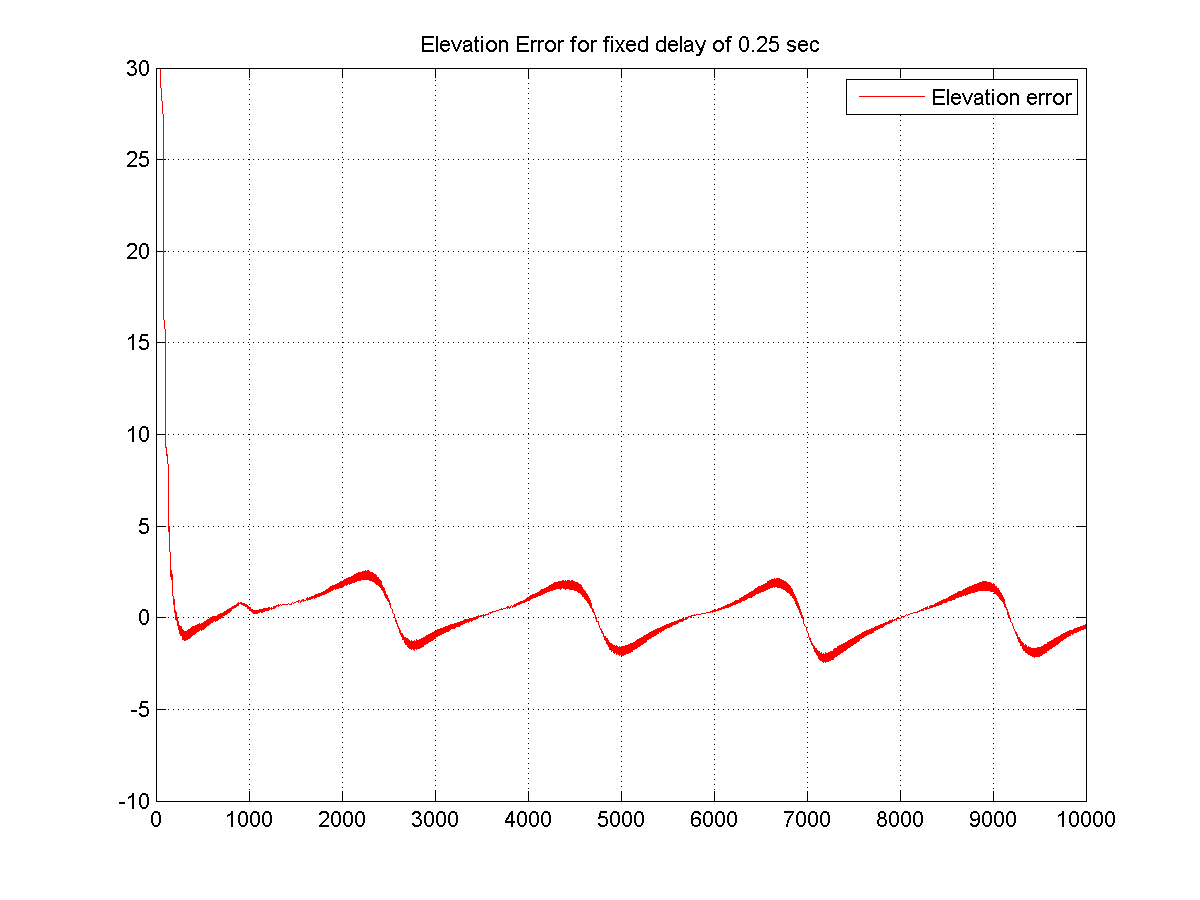
\includegraphics[scale=0.6]{./GPS_EKF/fixed_delay_0.25/fig11}
%  \caption{Elevation Error - Case 4}
%  \label{fig:theFig}
%\end{figure}
%\begin{figure}[h!]
%  \centering
%  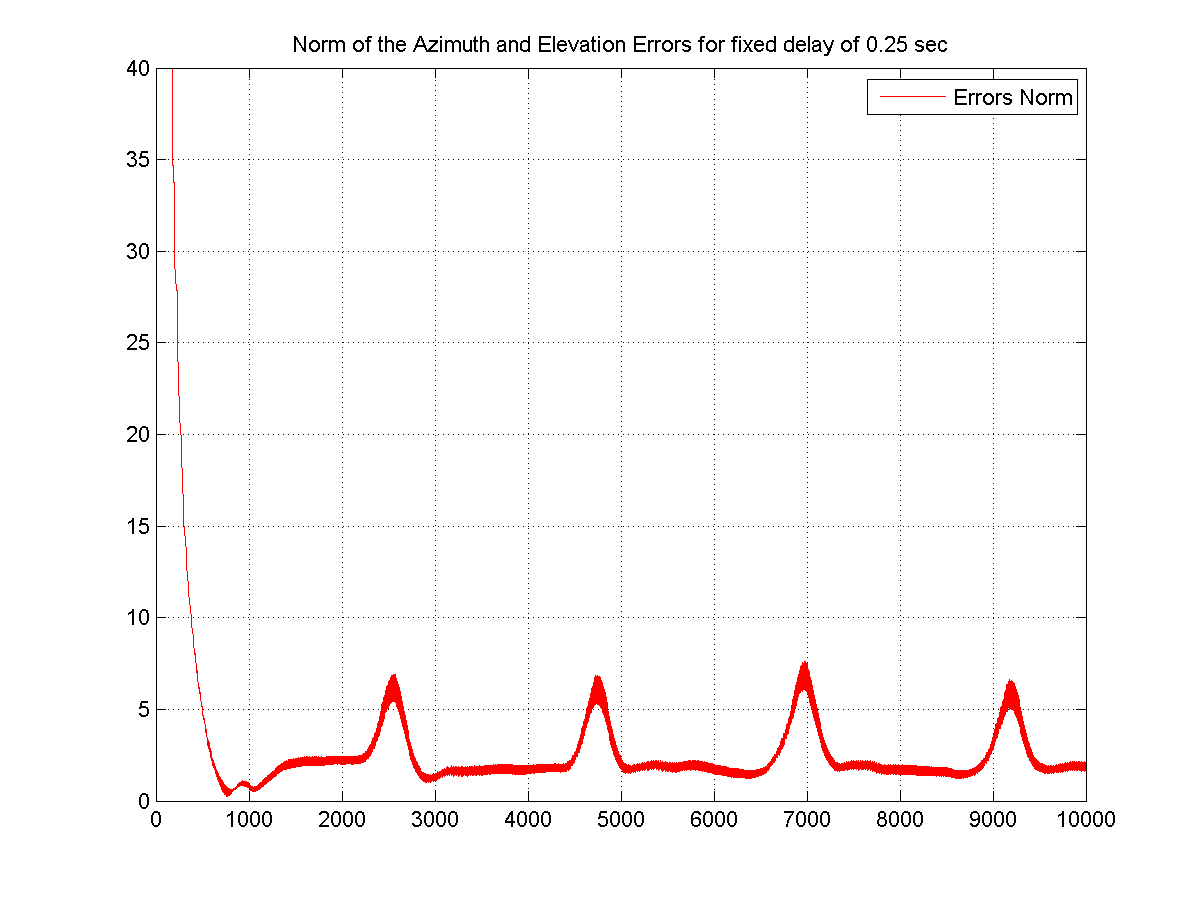
\includegraphics[scale=0.6]{./GPS_EKF/fixed_delay_0.25/fig12}
%  \caption{Normalized Azimuth and Elevation Errors - Case 4}
%  \label{fig:theFig}
%\end{figure}
%
%\subsection{Case 5 - GPS Sensor Coupled with Camera With Fixed Delay of 0.25 sec} \hspace{0pt} \\
%The camera and the GPS measurements are used in this scenario, where the GPS measurements have a delay of 0.25 s.
%
%\begin{figure}[h!]
%  \centering
%  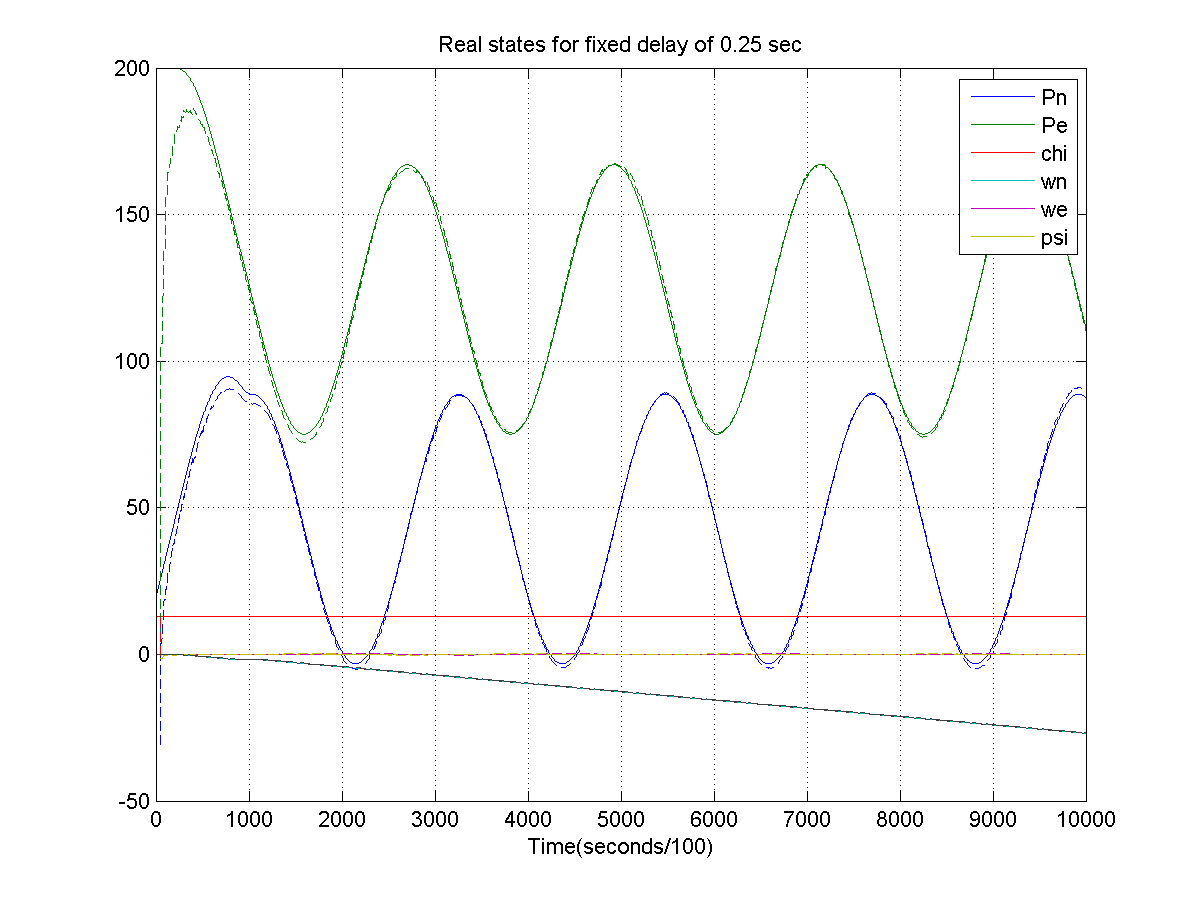
\includegraphics[scale=0.6]{./GPS_Cam/fixed_delay_0.25/fig4}
%  \caption{Real States vs Estimated States - Case 5}
%\end{figure}
%\pagebreak
%\begin{figure}[h!]
%  \centering
%  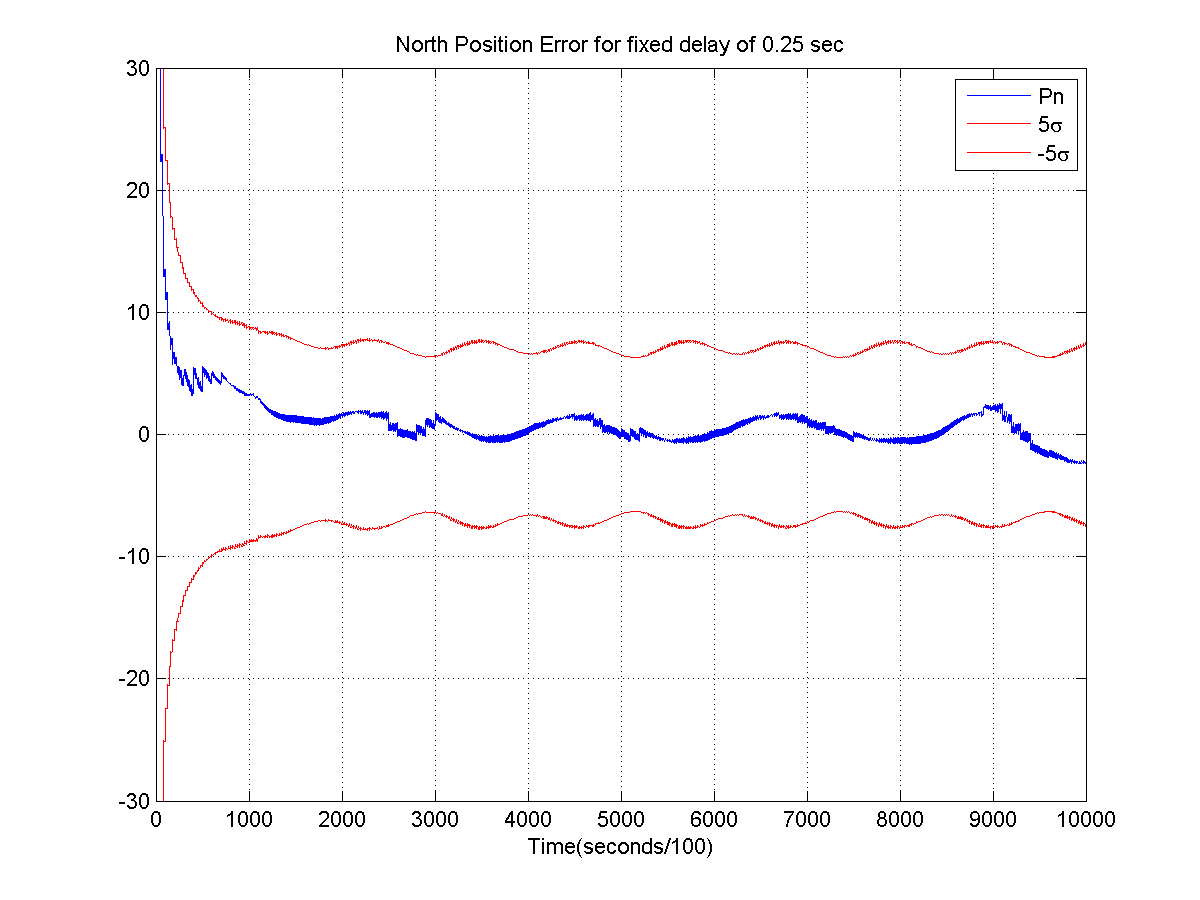
\includegraphics[scale=0.6]{./GPS_Cam/fixed_delay_0.25/fig5}
%  \caption{North Position Error - Case 5}
%\end{figure}
%\begin{figure}[h!]
%  \centering
%  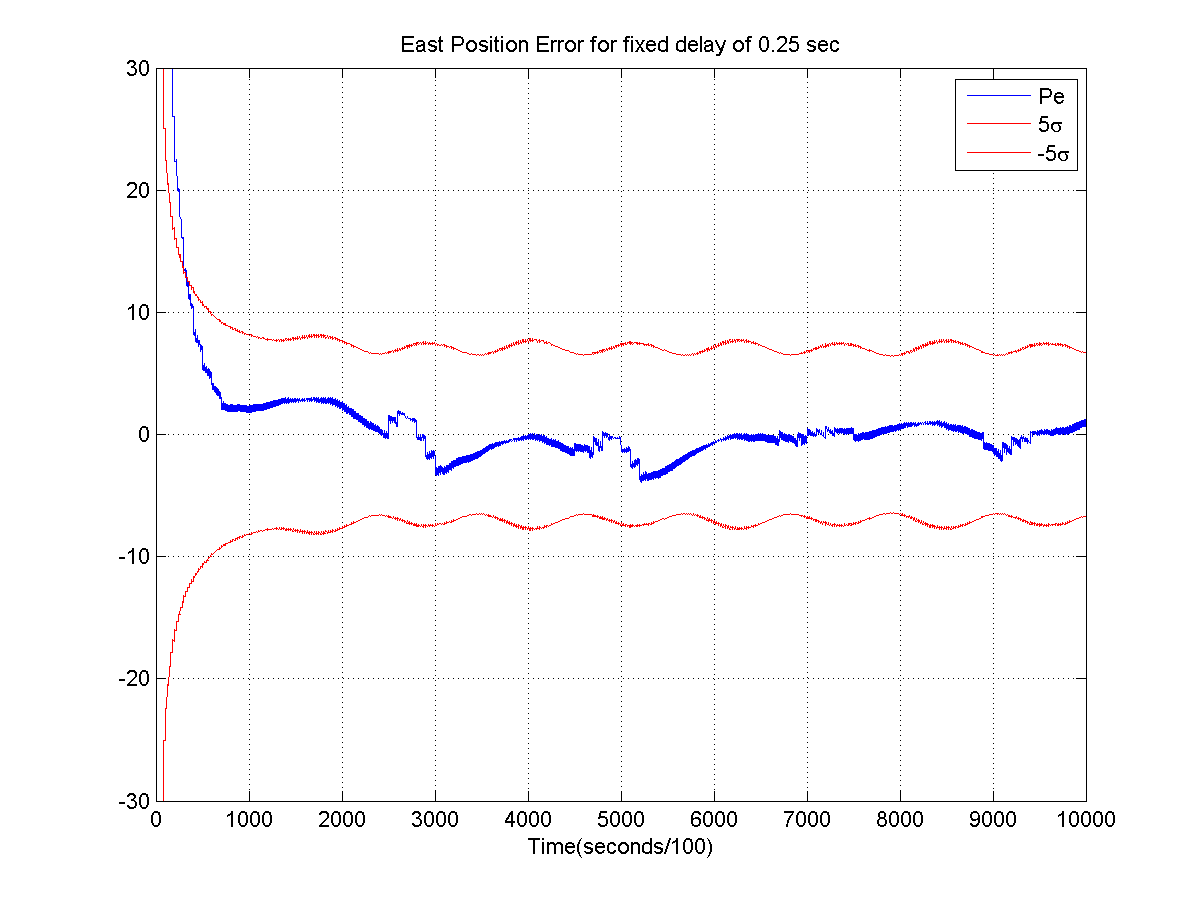
\includegraphics[scale=0.6]{./GPS_Cam/fixed_delay_0.25/fig6}
%  \caption{East Position Error - Case 5}
%  \label{fig:theFig}
%\end{figure}
%\begin{figure}[h!]
%  \centering
%  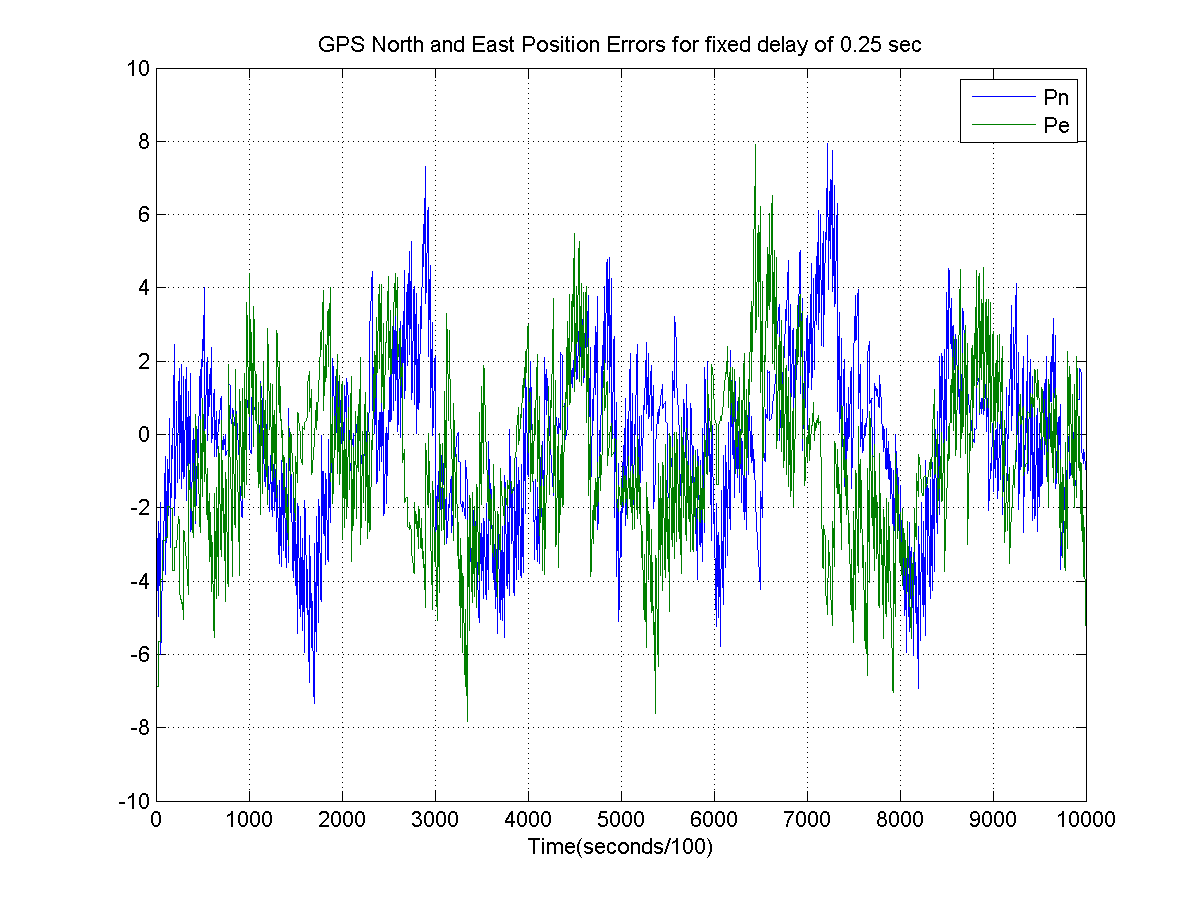
\includegraphics[scale=0.6]{./GPS_Cam/fixed_delay_0.25/fig7}
%  \caption{GPS Position Error - Case 5}
%  \label{fig:theFig}
%\end{figure}
%
%\begin{figure}[h!]
%  \centering
%  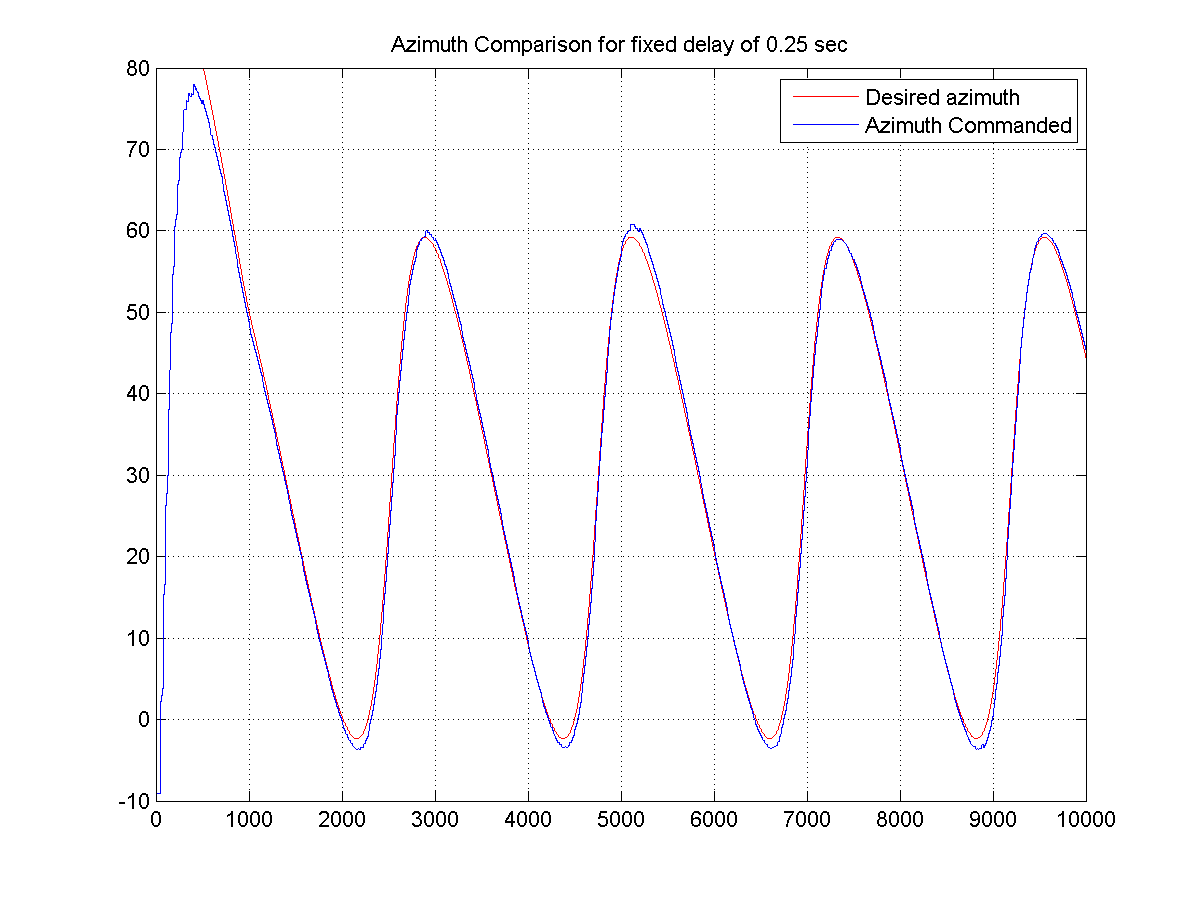
\includegraphics[scale=0.6]{./GPS_Cam/fixed_delay_0.25/fig8}
%  \caption{Desired Azimuth vs Estimated Azimuth - Case 5}
%  \label{fig:theFig}
%\end{figure}
%\begin{figure}[h!]
%  \centering
%  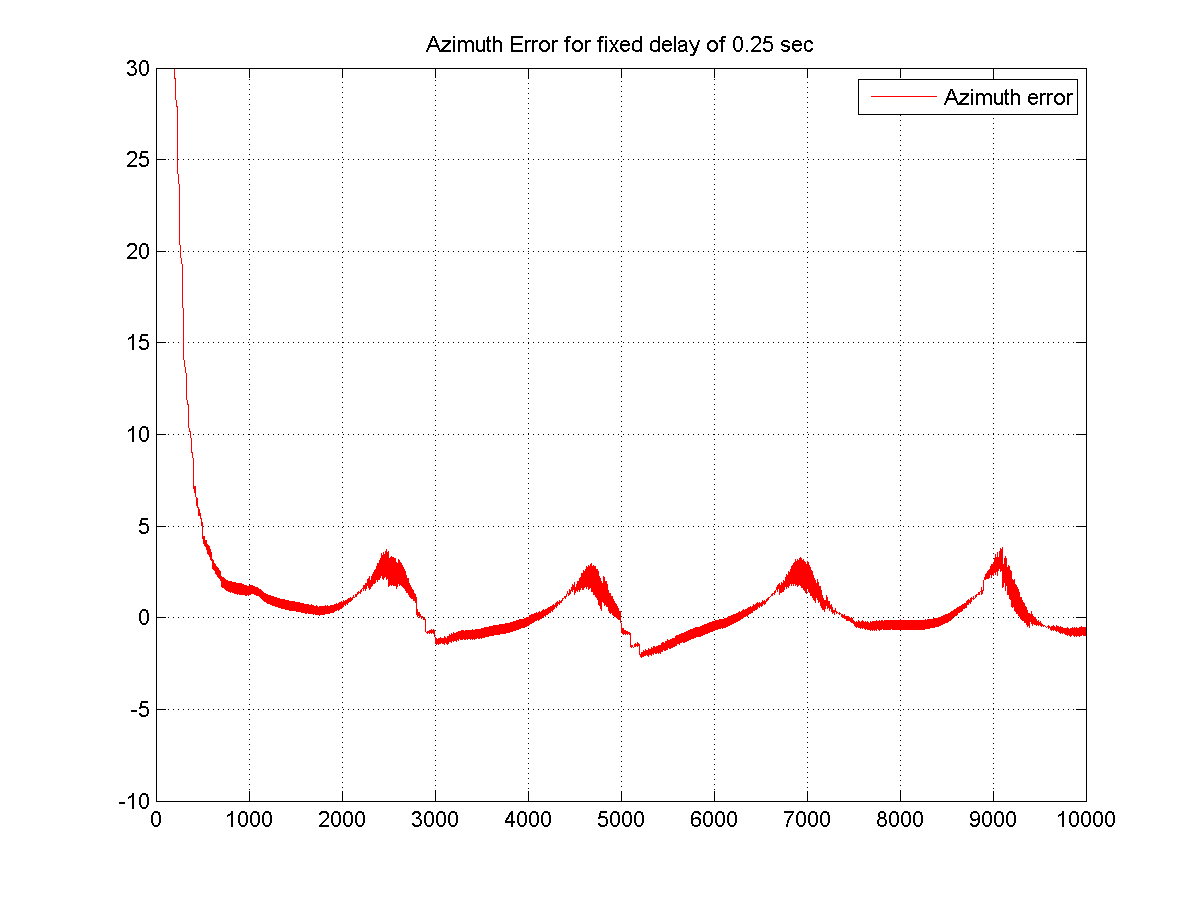
\includegraphics[scale=0.6]{./GPS_Cam/fixed_delay_0.25/fig9}
%  \caption{Azimuth Error - Case 5}
%  \label{fig:theFig}
%\end{figure}
%\begin{figure}[h!]
%  \centering
%  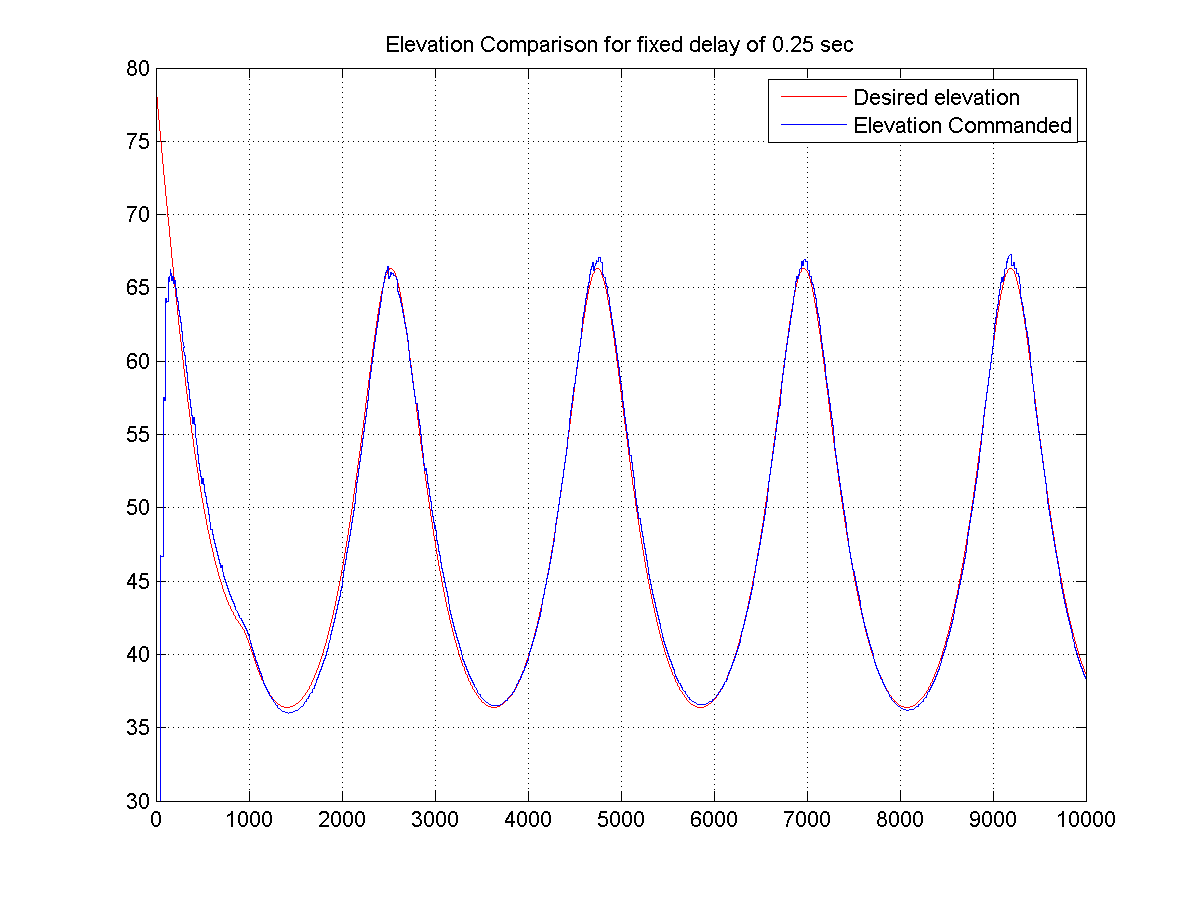
\includegraphics[scale=0.6]{./GPS_Cam/fixed_delay_0.25/fig10}
%  \caption{Desired Elevation vs Estimated Elevation - Case 5}
%  \label{fig:theFig}
%\end{figure}
%\begin{figure}[h!]
%  \centering
%  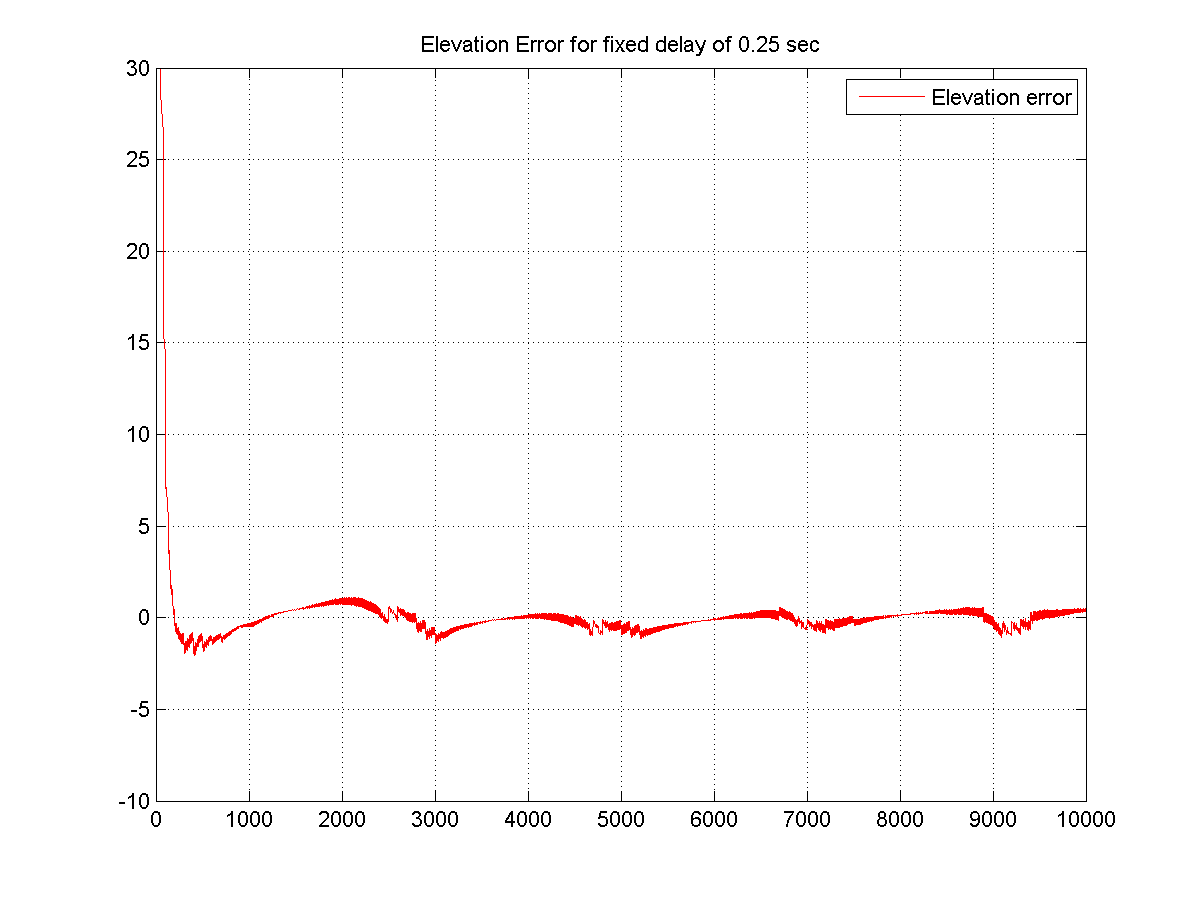
\includegraphics[scale=0.6]{./GPS_Cam/fixed_delay_0.25/fig11}
%  \caption{Elevation Error - Case 5}
%  \label{fig:theFig}
%\end{figure}
%
%\begin{figure}[h!]
%  \centering
%  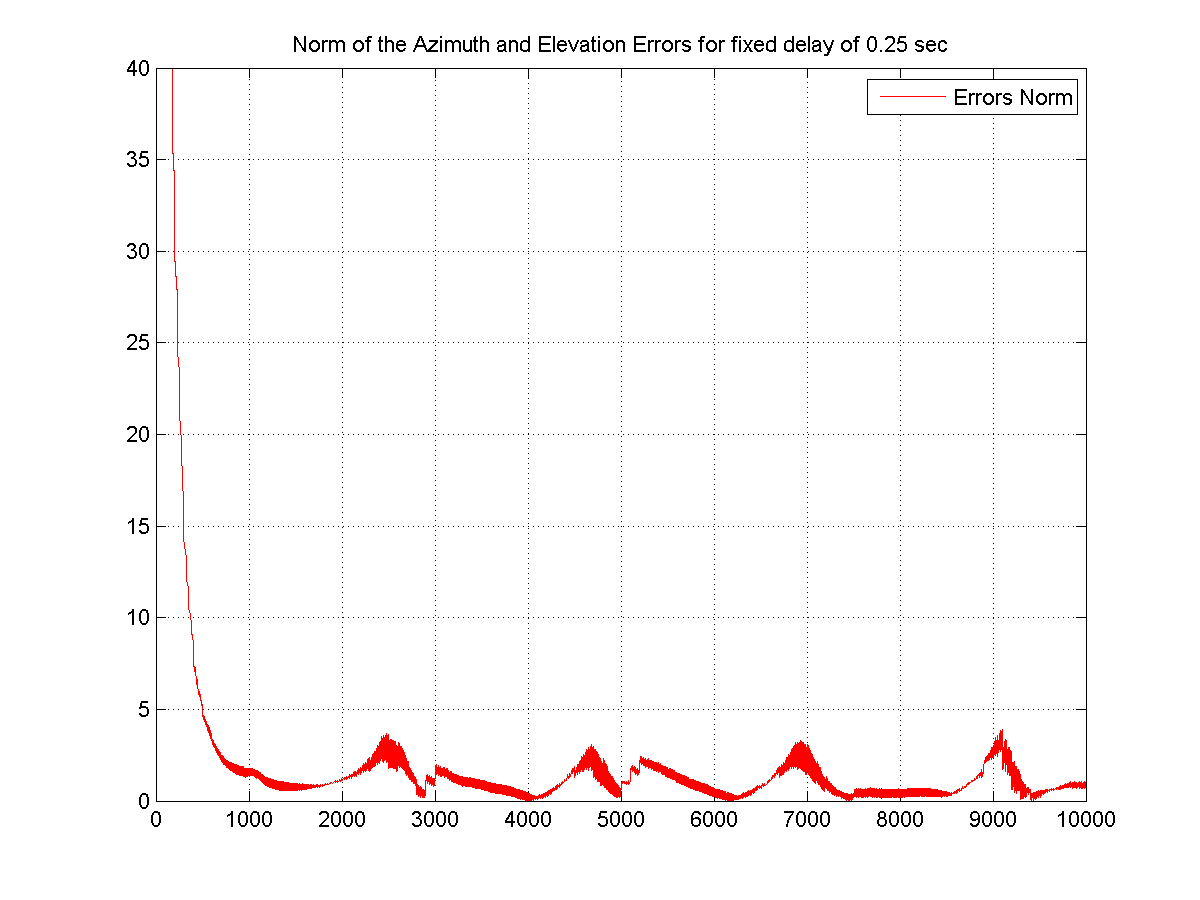
\includegraphics[scale=0.6]{./GPS_Cam/fixed_delay_0.25/fig12}
%  \caption{Normalized Azimuth and Elevation Errors - Case 5}
%  \label{fig:theFig}
%\end{figure}
%\subsection{Case 6 - GPS Sensor Coupled with Camera With Fixed Delay of 0.25 sec Disregarding Delay} \hspace{0pt} \\
%The camera and the GPS measurements are used in this scenario with the same delay as the previous case. Again we disregard the delay for comparison purposes.
%
%\subsection{Case 7 - GPS Sensor With Random Delay Up To 0.25 sec} \hspace{0pt} \\
%For this scenario, the delays are randomized with a maximum of 0.25 s. The changes in the estimate can be seen when the randomization is introduced. This situation is similar of what can be seen in the real world.
%\subsection{Case 8 - GPS Sensor With Random Delay Up To 0.25 sec Disregarding Delay} \hspace{0pt} \\
%
%\subsection{Case 9 - GPS Sensor Coupled with Camera With Random Delay Up To 0.25 sec} \hspace{0pt} \\
%
%\subsection{Case 10 - GPS Sensor Coupled with Camera With Random Delay Up To 0.25 sec Disregarding Delay} \hspace{0pt} \\
%
%\subsection{Case 11 - GPS Sensor With Fixed Delay of 0.50 sec} \hspace{0pt} \\
%
%\subsection{Case 12 - GPS Sensor With Fixed Delay of 0.50 sec Disregarding Delay} \hspace{0pt} \\
%
%\subsection{Case 13 - GPS Sensor Coupled with Camera With Fixed Delay of 0.50 sec} \hspace{0pt} \\
%
%\subsection{Case 14 - GPS Sensor Coupled with Camera With Fixed Delay of 0.50 sec Disregarding Delay} \hspace{0pt} \\
%
%\subsection{Case 15 - GPS Sensor With Out-Of-Sequence Measurements and Random Delay Up To 0.50 sec} \hspace{0pt} \\
%In this scenario the delay is randomized with a maximum of 0.50 s. Since in this time span the GPS sends two measurements, they could arrive with their order swapped, depending on the delay of each measurement. Here the Out-Of-Sequence Measurement problem explained before, arises.
%
%\subsection{Case 16 - GPS Sensor With Out-Of-Sequence Measurements and Random Delay Up To 0.50 sec  Disregarding Delay} \hspace{0pt} \\
%
%\subsection{Case 17 - GPS Sensor Coupled with Camera With Out-Of-Sequence Measurements and Random Delay Up To 0.50 sec} \hspace{0pt} \\
%
%\subsection{Case 18 - GPS Sensor Coupled with Camera With Out-Of-Sequence Measurements and Random Delay Up To 0.50 sec Disregarding Delay} \hspace{0pt} \\
%
%\subsection{Case 19 - GPS Sensor With Fixed Delay of 0.75 sec} \hspace{0pt} \\
%
%\subsection{Case 20 - GPS Sensor With Fixed Delay of 0.75 sec Disregarding Delay} \hspace{0pt} \\
%
%\subsection{Case 21 - GPS Sensor Coupled with Camera With Fixed Delay of 0.75 sec} \hspace{0pt} \\
%\subsection{Case 22 - GPS Sensor Coupled with Camera With Fixed Delay of 0.75 sec Disregarding Delay} \hspace{0pt} \\
%
%\subsection{Case 23 - GPS Sensor With Out-Of-Sequence Measurements and Random Delay Up To 0.75 sec} \hspace{0pt} \\
%In this case the maximum delay is increased to 0.75 sec. Now there are three measurements that could arrive out of order, therefore increasing the occurrence of the Out-Of-Sequence Measurement problem. 
%
%\subsection{Case 24 - GPS Sensor With Out-Of-Sequence Measurements and Random Delay Up To 0.75 sec  Disregarding Delay} \hspace{0pt} \\
%
%\subsection{Case 25 - GPS Sensor Coupled with Camera With Out-Of-Sequence Measurements and Random Delay Up To 0.75 sec} \hspace{0pt} \\
%
%\subsection{Case 26 - GPS Sensor Coupled with Camera With Out-Of-Sequence Measurements and Random Delay Up To 0.75 sec Disregarding Delay} \hspace{0pt} \\
%
%\subsection{Case 27 - GPS Sensor With Fixed Delay of 1 sec} \hspace{0pt} \\
%In this case, the delay is once more incremented, now to 1 s. The estimation is still acceptable but it can cross the sigma bound if the GPS error increases too much. 
%
%\subsection{Case 28 - GPS Sensor With Fixed Delay of 1 sec Disregarding Delay} \hspace{0pt} \\
%
%\subsection{Case 29 - GPS Sensor Coupled with Camera With Fixed Delay of 1 sec} \hspace{0pt} \\
%
%\subsection{Case 30 - GPS Sensor Coupled with Camera With Fixed Delay of 1 sec Disregarding Delay} \hspace{0pt} \\
%
%\subsection{Case 31 - GPS Sensor With Out-Of-Sequence Measurements and Random Delay Up To 1 sec} \hspace{0pt} \\
%
%\subsection{Case 32 - GPS Sensor With Out-Of-Sequence Measurements and Random Delay Up To 1 sec  Disregarding Delay} \hspace{0pt} \\
%
%\subsection{Case 33 - GPS Sensor Coupled with Camera With Out-Of-Sequence Measurements and Random Delay Up To 1 sec} \hspace{0pt} \\
%
%\subsection{Case 34 - GPS Sensor Coupled with Camera With Out-Of-Sequence Measurements and Random Delay Up To 1 sec Disregarding Delay} \hspace{0pt} \\

    \include{discussion}
    \chapter{Conclusion}
\label{ch:conclusion}

%La conclusion debe tener una estructura clara la cual pueda mantener la atencion del lector y proveer una sequencia convincente de como el estudio puede inequivocamente y rigurosamente identificar conocimiento que permite sustentar la teoria.
%La conclusion, al igual que la tesis, debe tener un inicio (introduccion), una seccion media (sintesis de los descubrimientos empiricos y respuestas de las preguntaste de la investigacion), implicaciones teoricas y un final (direcciones para investigaciones futuras).

%Estrategias para desarrollar una buena introduccion:
%-Empieza con una oracion que haga referencia al tema principal de la tesis.
%-Indica la importancia del tema en cuestion
%-Reafirma las preguntas de la investigacion como fueron presentadas en el capitulo introductorio.


The purpose of this study was to develop an algorithm which could point an antenna and a camera towards a UAS. The reasons and motivations to this problem are primarily two. The first motivation was the Line-Of-Sight requirement of the Federal Aviation Administration which limits UAV missions to operate if and only if the aircraft is in the field of view of the operator. The existing method, is to keep an eye on the UAV with binoculars, which is prone to miss the plane frequently. Likewise, the other reason for the study was to improve the reliability of the mission by assuring the communication link with the aircraft, which can be achieved with a trustworthy tracking system. \linebreak
\linebreak
The main hypotheses that we had were the following three.
\begin{enumerate}
\item The coupling of a camera with a GPS improves the state estimations of an aircraft.
\item Delayed and out of sequence measurements affect the state estimations in an inversely proportional way. A special Kalman filter needs to be used to address this scenario.
\end{enumerate}
With the empirical findings we were able to conclude that:
\begin{enumerate}
\item If a camera is coupled with a GPS for state estimation in a Kalman filter, the errors will be less than those of using a GPS alone. This is more evident when the GPS measurements are delayed.
\item State estimations are adversely affected by an increase of delays in the measurements. Errors were significantly decreased when a special filter called Delayed Extended Kalman filter was used, opposed to using the regular Extended Kalman filter.
\end{enumerate}
\pagebreak

One of the impacts of this study is the possibility of a modification of the Line-Of-Sight requirement of the FAA, allowing tracking systems to comply with this regulation as long as they are equipped with a camera. Therefore, freeing the operator of this task. Furthermore, tracking systems could implement these findings to improve their robustness, making more reliable the mission as a whole.

This research could be extended with the implementation of the antenna pointer system, to run more extensively tests. On the other hand, the same principle could be analyzed where the only sensors available were a camera and a signal strength receiver. Moreover, a scenario where communication or measurements are lost could be an interesting case of study.

This thesis has offered an approach to UAV tracking systems to improve the existing process, and was conducted in a simulated platform, MATLAB and Simulink, to have a strictly controlled environment. For simplifying purposes we made two main assumptions that need to be mentioned. One of the premises was that there was an image recognition algorithm which always recognized the aircraft as long as it were in the field-of-view of the camera. The second assumption was that the delays in the camera measurements were so small that they could be neglected without a big impact of the estimations.

As a support of what is often reasoned, an algorithm which consider the delays in the measurements and the OOSM problem, such as the Delayed Extended Kalman filter, reduces the estimates errors. Hence, a system which regards these conditions, can efficiently track a UAS increasing the reliability of the whole mission.

    \references{IEEEabrv,library}{IEEEtran}
    
    %%
%  Example Appendix pages.
%  Modified to use new usu-thesis-mk2 appendix facilities.
%
%  Time-stamp: "[appendix.tex] last modified by Scott Budge (scott) on 2011-08-08 (Monday, 8 August 2011) at 15:46:06 on goga"
%
%  Info: $Id$   USU
%  Revision: $Rev$
% $LastChangedDate$
% $LastChangedBy$
%
%
% For a single appendix, use \makeappendix, and place the 
% body of the appendix after it

%\makeappendix

% < single appendix body here >

% For multiple appendices, use \makeappendices, and create each appendix
% using \appendix{}
% For sub-appendices use \appendixsection{} and \appendixsubsection{}

\makeappendices
\appendix{List of Edge Vectors}
\label{chap:appendix}


\appendixsection{Definition of an Edge Vector}
\label{sec:edge-def}

Before we list the table of edge vectors, we need to describe what an
edge vector is.  In this section we will describe in detail the theory
that results in the edge vectors.  The first set of edge vectors is
given in Table~\ref{table1}.

\begin{table}[!t]
% increase table row spacing, adjust to taste
  \renewcommand{\arraystretch}{1.3}

  \caption{List of edge vectors for a codebook with b=8 and d=3, for a
    $4 \times 4$ vector size.}
  \label{table1}

  \centering
  \begin{tabular}{|c|c|} \hline
    Level & Edge Vectors \\ \hline

    & (5) \\ 
    L1 & (6) \\
    & (7) \\ \hline

    & (3,1)\\
    & (3,2)\\
    & (3,5)\\
    & (4,0)\\
    L2 & (4,2)\\
    & (4,3)\\
    & (4,4)\\
    & (4,5)\\
    & (4,6) \\ \hline

    & (3,4,1)\\
    & (3,4,2)\\
    & (3,7,0)\\
    & (3,7,2)\\
    & (3,7,4)\\
    L3 & (4,1,0)\\
    & (4,1,1)\\
    & (4,1,2)\\
    & (4,1,3)\\
    & (4,1,4)\\
    & (4,1,5)\\
    & (4,1,6) \\ \hline

  \end{tabular}

\end{table}


\appendixsection{Next Codebook Size Description}
\label{sec:next-size}

In this section we do the next size codebook.  This is different from
the previous case in that the codebook size is different.  The next
set of edge vectors is given in Table \ref{table2}.

\appendixsection{Final Set of  Codebook Size Descriptions}
\label{sec:final-size}

The following three tables contain the data for codebook sizes that
are different than the previous sizes.  We note that the differences
in the tables are due to the differences in the sizes of the codebook
edge vectors.  Note the values given in Table \ref{table3} --
Table \ref{table5}.


\begin{table}[!t]
  \renewcommand{\arraystretch}{1.3}
  \centering

  \caption{List of edge vectors for a codebook with b=4 and d=3, for a
    $4 \times 4$ vector size.}
  \label{table2}

  \begin{tabular}{|c|c|} \hline
    Level & Edge Vectors \\ \hline

    & (1)\\
    L1 & (2)\\
    & (3) \\ \hline

    L2 & (0,3) \\ \hline

    & (0,2,0)\\
    L3 & (0,2,2)\\
    & (0,2,3) \\ \hline

  \end{tabular}

\end{table}

\begin{table}[!t]
  \renewcommand{\arraystretch}{1.3}
  \centering

  \caption{List of edge vectors for a codebook with b=16 and d=3, for
    a $4 \times 4$ vector size.}
  \label{table3}

  \begin{tabular}{|c|c|} \hline
    Level & Edge Vectors \\ \hline

    & (11)\\
    & (12)\\
    L1 & (13)\\
    & (14)\\
    & (15) \\ \hline

    & (7,0)\\
    & (7,1)\\
    & (7,2)\\
    & (7,6)\\
    L2 & (8,4)\\
    & (8,5)\\
    & (8,6)\\
    & (9,6)\\
    & (9,14)\\
    & (10,1) \\ \hline

    & (4,6,14)\\
    & (5,6,6)\\
    & (6,14,0)\\
    & (6,14,3)\\
    L3 & (6,14,4)\\
    & (6,14,5)\\
    & (7,7,0)\\
    & (7,14,7)\\
    & (9,5,3)\\
    & (9,5,10)\\
    & (9,5,11) \\ \hline

  \end{tabular}

\end{table}

\begin{table}[!t]
  \renewcommand{\arraystretch}{1.3}
  \centering

  \caption{ List of edge vectors for a codebook with b=16 and d=3, for
    a $2 \times 2$ vector size.}
  \label{table4}

  \begin{tabular}{|c|c|} \hline
    Level & Edge Vectors \\ \hline

    & (9)\\
    & (10)\\
    L1 & (11)\\
    & (12)\\
    & (13) \\ \hline

    L2 & (6,0)\\
    & (6,3) \\ \hline

    & (2,2,8)\\
    & (6,5,1)\\
    & (6,5,4)\\
    & (6,5,6)\\
    & (6,5,7)\\
    & (6,5,8)\\
    L3 & (6,5,15)\\
    & (7,0,14)\\
    & (8,0,1)\\
    & (8,15,3)\\
    & (8,15,4)\\
    & (8,15,10) \\ \hline

  \end{tabular}

\end{table}

\begin{table}[!t]
  \renewcommand{\arraystretch}{1.3}
  \centering

  \caption{ List of edge vectors for a codebook with b=16 and d=3, for
    a $6 \times 6$ vector size.}
  \label{table5}

  \begin{tabular}{|c|c|} \hline
    Level & Edge Vectors \\ \hline

    & (6)\\
    & (7)\\
    & (8)\\
    & (9)\\
    L1 & (10)\\
    & (11)\\
    & (12)\\
    & (13)\\
    & (14)\\
    & (15) \\ \hline

    & (2,8)\\
    & (2,13)\\
    & (4,1)\\
    & (4,6)\\
    L2 & (4,7)\\
    & (4,8)\\
    & (4,10)\\
    & (4,11)\\
    & (4,13)\\
    & (4,15) \\ \hline

    & (1,7,0)\\
    & (1,7,1)\\
    & (1,7,2)\\
    L3 & (1,7,3)\\
    & (1,7,4)\\
    & (1,7,6)\\
    & (1,7,9)\\
    & (1,7,12) \\ \hline

  \end{tabular}

\end{table}

\appendix{Another Example Appendix}


\appendixsection{Background}
\label{sec:back}


Some random appended text for this section of the appendix....


\appendixsection{Meat of the Appendix}
\label{sec:meat}

Here we have the data that is so important to be included in this
appendix.

%    \include{vita}
    %}}}
\end{document}
